\documentclass[a4paper, 11pt]{book}
\usepackage[margin=1in]{geometry}
% \usepackage[a4paper, total={6.7in, 8in}]{geometry}
% \usepackage[margin=0.5in]{geometry}

%\usepackage{fontspec}
\usepackage{lmodern}
\usepackage{lipsum}
\usepackage{psl-cover}

% my packages:
\usepackage[utf8]{inputenc}
\usepackage[english]{babel}
\usepackage{amsmath}
\usepackage{amsfonts}
\usepackage{amssymb}
\usepackage{graphicx}
\usepackage{siunitx}
\sisetup{math-micro=\text{µ},text-micro=µ}
\usepackage[euler]{textgreek}
\usepackage{subcaption}
\usepackage{booktabs}
\usepackage{soul}
\usepackage{enumitem}
\usepackage{bm}

\usepackage{import}
\usepackage{example}
\usepackage{graphicx}
\usepackage{amsmath}
\usepackage{float}
\usepackage{amssymb}
\usepackage{xcolor}
\usepackage{hyperref}
\usepackage{longtable}
\usepackage{../notations}
\usepackage{listings}
\usepackage{multicol}
\usepackage{import}
\usepackage{comment}
% \usepackage{cancel}
\usepackage{ulem}
\usepackage{booktabs,xltabular}
\usepackage{longtable}

\title{Insérer ici l'intitulé du sujet de thèse}

\author{Martinus Putra Widjaja}

\institute{MINES ParisTech}
\doctoralschool{Ingénierie des Systèmes, Matériaux, Mécanique, Energétique}{621}
\specialty{Voir spécialités ED}
\date{jj mois aaaa}

% cotutelle
% \entitle{Thesis Sub lay}
% \logootherinstitute{logo-institute}

\jurymember{1}{Prénom NOM}{Titre, établissement}{Président}
\jurymember{2}{Prénom NOM}{Titre, établissement}{Rapporteur}
\jurymember{3}{Prénom NOM}{Titre, établissement}{Rapporteur}
\jurymember{4}{Prénom NOM}{Titre, établissement}{Examinateur}
\jurymember{5}{Prénom NOM}{Titre, établissement}{Examinateur}
\jurymember{6}{Prénom NOM}{Titre, établissement}{Examinateur}
\jurymember{7}{Prénom NOM}{Titre, établissement}{Examinateur}
\jurymember{8}{Alain THIONNET}{Titre, établissement}{Directeur de thèse}
% \jurymember{9}{Prénom NOM}{Titre, établissement}{Invité}
% \jurymember{10}{Prénom NOM}{Titre, établissement}{Invité}

\input{abstract}

\begin{document}

\maketitle{}

\tableofcontents
\listoffigures

\chapter{Introduction}

\section{Industrial Context}

\subsection{The fuel element of pressurized water reactor}

The industrial French nuclear fleet is made of Pressurized Water Reactor
(PWR), as well as three quarters of power reactors worldwide.

A fuel element is a stack of fuel pellets enclosed in a cladding made of
an alloy of Zirconium. This fuel element is thus called a fuel rod. A
fuel rod is almost 4 meters long, and the cladding outer diameter is
$9.5$mm wide.

% ![Typical dimensions of a fuel pellet](img/FuelPellet.pdf ""){#fig:hho:fuel_pellet width=75%}

\begin{figure}[H]
  \centering
  \includegraphics[width=10.cm]{../chapter_000_introduction/figures/FuelPellet.pdf}
  \caption{Typical dimensions of a fuel pellet}
  \label{fig:hho:fuel_pellet}
\end{figure}

The fuel pellet itself is mostly made of Uranium dioxide \(UO_{2}\) or a
Mixed Oxide (MOX) which also incorporates Plutonium. The typical
dimensions of a fuel pellet are reported on Figure \ref{fig:hho:fuel_pellet}.
The main nuclear reaction in the fuel is the fission of dioxide
\(\mbox{}^{235}U\) isotope of Uranium and in several isotopes
of Plutonium. The presence of dishings have significant influence on the
behaviour of the pellet in power transient, as discussed in Section
\ref{sec:hho:off_normal_operating_conditions}.

Fuels rod are gathered in an assembly which typically holds \(264\) fuel
rods. In a \(900\,MWe\) PWR, the core contains \(157\) assemblies for a
total of approximatively \(41\,000\) fuels rods.

In the reactor core, the fuel rod is surrounded by pressurized water (at
around \(15,5\, MPa\) and a temperature of about $320$°C). The role of the
pressurized water is twofold:

\begin{itemize}
    \item Thermalizing neutrons, i.e. absorbing part of a neutron energy down to
    a level for which the cross-section of \(\mbox{}^{235}U\) is
    significantly higher \footnote{Fission cross section of \(\mbox{}^{235}U\) for slow thermal
    neutrons is about \(584\) barns which is significantly higher that the
    cross-section of fast neutrons which is typically on the order of 1
    barn.}.
    \item Extracting the heat generated by those reactions. Hence, the water in
    the reactor core is generally denoted as the coolant.
\end{itemize}

% \footnotetext[U235]{Fission cross section \(\mbox{}^{235}U\) of for slow thermal
% neutrons is about \(584\) barns which is significantly higher that the
% cross-section of fast neutrons which is typically on the order of 1
% barn.}

% - Thermalizing neutrons, i.e. absorbing part of a neutron energy down to
%   a level for which the cross-section of \(\mbox{}^{235}U\) is
%   significantly higher[^U235].
% - Extracting the heat generated by those reactions. Hence, the water in
%   the reactor core is generally denoted as the coolant.

% [^U235]: Fission cross section \(\mbox{}^{235}U\) of for slow thermal
% neutrons is about \(584\) barns which is significantly higher that the
% cross-section of fast neutrons which is typically on the order of 1
% barn.

From a safety point of view, the integrity of the cladding, i.e. its
ability to retain the fuel from disseminating radioactive elements in
the coolant, must be assessed.

This point is studied by the experimental campaigns in research reactors
and the development of simulation tools worldwide
\cite{garcia_mono-dimensional_2002, williamson_multidimensional_2012, di_marcello_transuranus_2014, largenton_cyrano3_2014, petry_cyrano3_2015, qi_qualification_2019,scolaro_offbeat_2020}.

In particular, CEA develops a numerical platform called \texttt{PLEIADES}
\cite{marelle_new_2016} to simulate the behaviour of nuclear fuel elements
for various nuclear systems (PWR, Sodium Fast Reactor, Material Testing Reactor) in normal and
off-normal operating conditions and also experimental devices
\cite{lainet_recent_2013, helfer_licos_2015}. In this platform, the
\texttt{ALCYONE} fuel performance code is dedicated to PWR fuels
\cite{helfer_recent_2015, marelle_new_2016, guenot-delahaie_simulation_2017}.

The precise understanding of the evolution of the fuel rod under
irradiation is made all the more difficult due to the numerous coupled
physical phenomena at play \cite{JRC83478}. The next section is
devoted to an overview of the fuel rod evolution under irradiation in
normal and off-normal operating conditions.

\subsection{A compendium of the fuel rod evolution under irradiation}

A complete description of fuel rod evolution under irradiation is out of
the scope of this document. The interested reader may refer to the
reference books on that matter for further details
\cite{bailly_nuclear_1999, cea_nuclear_2009}. This paragraph only presents
the most relevant phenomena occurring in the fuel rod in the perspective
of our work.

\paragraph{Normal operating conditions}
\label{sec:hho:normal_operating_conditions}

Nuclear reactions in the fuel lead to an important temperature gradient
in the fuel pellet. For a nominal power of about \(200\,W.cm^{-1}\),
this radial gradient is typically greater than \(100\,K.mm^{-1}\). This
temperature gradient induces a high level of stresses by
thermoelasticity:

\begin{itemize}
    \item The center, which is around \(1\,400\, K\), of the pellet is in
    compression.
    \item The periphery of the pellet, which is around \(1\,000\,K\), is in
    tension.
\end{itemize}

% ![Simplified classification of the observed cracks (left). Initial
% fragmentation of the fuel pellet simulated using a phase field approach
% \cite{2019_LU_HELFER_BARY_FANDEUR_UnSchemaNumeriqueEfficacePourLeTraitementDeLaFissurationFragileDesMateriauxQuasiFragilesParChampDePhase} (right). Because of a coarse mesh, this
% simulation is not totally representative of the fracture properties of
% \(UO_{2}\), i.e. the characteristic length used in the simulation, which
% must be greater than the mesh size, is too high (See Section
% @sec:phase_field:crack_nucleation). However, these simulations capture
% qualitatively the experimental crack patterns.](img/CrackNetwork.pdf ""){#fig:hho:crack_network with=75%}

\begin{figure}[H]
  \centering
  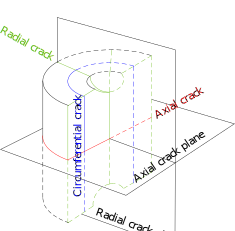
\includegraphics[width=10.cm]{../chapter_000_introduction/figures/CrackNetwork.pdf}
  \caption{Simplified classification of the observed cracks (left). Initial
  fragmentation of the fuel pellet simulated using a phase field approach
  \cite{2019_LU_HELFER_BARY_FANDEUR_UnSchemaNumeriqueEfficacePourLeTraitementDeLaFissurationFragileDesMateriauxQuasiFragilesParChampDePhase} (right). Because of a coarse mesh, this
  simulation is not totally representative of the fracture properties of
  \(UO_{2}\), i.e. the characteristic length used in the simulation, which
  must be greater than the mesh size, is too high (See Section
  \ref{sec:phase_field:crack_nucleation}). However, these simulations capture
  qualitatively the experimental crack patterns}
  \label{fig:hho:crack_network}
\end{figure}

The induced stresses far exceeds the fracture strength of Uranium
dioxide. Due to the brittle nature of Uranium dioxide, a complex cracks
network propagates in the pellet. A simple thermoelastic computation
shows that the fracture stress is reached during the reactor start-up
\cite{helfer_etude_2006}. A schematic representation of the cracked pellet,
using conventions of Figure \ref{fig:hho:crack_network} is currently used in
most \(3D\) simulations performed with the \texttt{Alcyone} fuel performance
code and can be built by inserting an axial crack in the mid-pellet
plane and \(6\) to \(8\) radial cracks, such that the fuel pellet is
divided into \(12\) to \(16\) macroscopic fragments. Most simulations
only consider half a fragment of pellet due to symmetry conditions
\cite{michel_pellet_2005}.

Numerically, initial fragmentation of the pellet has been studied in
\cite{helfer_modelisation_2017} and later by Lu et al. \cite{2019_LU_HELFER_BARY_FANDEUR_UnSchemaNumeriqueEfficacePourLeTraitementDeLaFissurationFragileDesMateriauxQuasiFragilesParChampDePhase} by a
phase field approach as depicted in Figure
\ref{fig:hho:crack_network}.

\begin{figure}[H]
  \centering
  \includegraphics[width=10.cm]{../chapter_000_introduction/figures/HourGlassEffect.pdf}
  \caption{Hourglass shape of the pellet. Initial shape is depicted using solid
  lines while the hourglass shape is depicted using dashed
  lines}
  \label{fig:hho:hourglass}
\end{figure}

% ![Hourglass shape of the pellet. Initial shape is depicted using solid
% lines while the hourglass shape is depicted using dashed
% lines.](img/HourGlassEffect.pdf){#fig:hho:hourglass width=50%}

The temperature gradient in the fragments leads to the hourglassing of
the pellet, i.e. the radial displacement of points of the outer surface
of the pellet is much greater in the inter-pellet plane than in the
mid-pellet plane (see Figure \ref{fig:hho:hourglass}). After fragmentation,
the remaining stresses in the fuel are relieved by irradiation creep.

The cladding is submitted to the pressure of the coolant which far
exceeds the initial pressure in the fuel rod. The cladding, whose
temperature is between \(560\,K\) and \(600\,K\), is in compression.
Viscoplasticity, accelerated under irradiation, leads to a reduction of
the radius of the cladding.

During the first and second operating cycles, the gap between the fuel
pellet and the cladding remains open but diminishes due to three
phenomena of equal importance:

\begin{itemize}
  \item The thermal expansion of the pellet.
  \item The hourglassing of the pellet.
  \item The viscoplastic flow in the cladding due to the coolant pressure.
\end{itemize}

During the first cycle, the initial porosity of the pellet diminishes due to the
in-pile densification leading to a decrease of the fuel pellet radius
which is compensated by swelling due to solid fission products.

After the first two cycles, the gap between the fuel pellet and the
cladding is closed and a weak interaction between the pellet and the
cladding occurs. Due to the hour-glass shape of the fuel pellet, this
interaction happens earlier in the inter-pellet plane. Due to the coolant
pressure, the pellet hourglassing diminishes, a phenomena also called
fragments' repositioning. Although the contact between the pellet and
the cladding is ultimately established on the whole outer surface of the
pellet, the earlier interaction in the inter-pellet plane is visible on
the cladding on which ridges appears. After irradiation, the cladding
thus has a "bamboo"-like shape.

After a few cycles, the cladding diameter increases due to fuel-pellet
swelling. The coolant pressure is gradually compensated by the inner
pressure increase in the fuel rod due to the release of gaseous fission
products. A high burn-up (micro-)structure develops at the periphery of
the pellet. This phenomenon is called the "rim"-effect. The high burn-up
structure affects various aspect of the fuel behaviour, including
viscoplasticity and swelling.

Many advanced models describe the behaviour of fission products and
microstructural evolutions of the fuel \cite{pizzocri_sciantix_2020}. In
particular, CEA has developed the \texttt{CARACAS} \cite{boulore_approach_2017}
and \texttt{MARGARET} models \cite{noirot_margaret_2011}.

For the purpose of this document, it shall be highlighted that all those
models take into account the macroscropic mechanical state of the pellet
through the hydrostatic pressure.

\paragraph{An example of off-normal operating conditions}
\label{sec:hho:off_normal_operating_conditions}

This paragraph is devoted to the description of a less severe off-normal
operating condition, namely power transient of class II. During this
class of transient, the power generated by the fuel rod may exceed
\(450\,W.cm^{-1}\) during a few hours. A typical evolution of the
maximum temperature in the fuel pellet is reported in Figure
\ref{fig:hho:transient_power}.

Several scenarii aimed at anticipating the consequences of off-normal
operating conditions are studied experimentally and numerically:

\begin{itemize}
  \item Reactivity Initiated Accident (RIA) describes the effect of an
  unwanted fast increase in fission rate and reactor power, due for
  example to the ejection of a control rod. Such situations can notably
  be reproduced experimentally in the Cabri research reactor located at
  CEA center of Cadarache where an experimental rod can be submitted to
  a power pulse of a few micro-seconds. Simulations of such pulses using
  the \texttt{Alcyone} fuel performance code are described in
  \cite{guenot-delahaie_simulation_2017}.
  \item Loss of coolant accidents (LOCAs) describe the consequence of a
  breach in the coolant circuit in which the cladding may not be cooled
  for a few minutes. Although the nuclear reaction may rapidly stop, the
  residual power generated by the fuel rod may lead to a significant
  increase of the cladding temperature. Such situations may notably be
  studied in the Halden research reactor. Simulations of such transients
  using the \texttt{Alcyone} fuel performance code are provided by
  \cite{struzik_simulation_2017}.
\end{itemize}

% ![Evolution of the maximim temperature during a power transient of class II in a research reactor](img/TransientPowerClassII.png){#fig:hho:transient_power width=75%}

\begin{figure}[H]
  \centering
  \includegraphics[width=10.cm]{../chapter_000_introduction/figures/TransientPowerClassII.png}
  \caption{Evolution of the maximim temperature during a power transient of class II in a research reactor}
  \label{fig:hho:transient_power}
\end{figure}

Swelling due to fission gas release induces an increase of cladding
radius which can lead to its failure.

% ![Typical crack network in the fuel pellet after irradiation in a research reactor](img/CrackNetwork2.pdf){#fig:hho:crack_network_2 width=75%}

\begin{figure}[H]
  \centering
  \includegraphics[width=10.cm]{../chapter_000_introduction/figures/CrackNetwork2.pdf}
  \caption{Typical crack network in the fuel pellet after irradiation in a research reactor}
  \label{fig:hho:crack_network_2}
\end{figure}

Figure \ref{fig:hho:crack_network_2} describes the typical metallographies of
a pellet after the power transient. While the primary crack network that
led to the pellet fragmentation is still visible, a secondary crack
network in the pellet appears. This secondary crack network may have a
significant and beneficial impact of the pellet-cladding interaction
during the power transient \cite{michel_3d_2008}.

Due to the viscoplasticity of the fuel at high temperature, an axial
movement of matter fills the dishings, leading to locally high strain
level. This viscoplastic behaviour of the core of the pellet also
significantly decreases the loading on the cladding.

Viscoplasticity at high temperature of uranimum dioxide, mostly
on unirradiated material, has been the subject of many studies,
including
\cite{colin_etude_2003,monerie_overall_2006, salvo_experimental_2015, salvo_experimental_2015-1, garcia_effect_2020}.

Simulations of such power transients with \texttt{Alcyone} are described in
\cite{helfer_etude_2006, michel_3d_2008}.

\subsection{Fuel behaviour at the microstructural scale}

% ![Description of the failure of a representative element volume due to
% the bubble pressurisation in the high burn-up structure
% \cite{esnoul_etude_2018}.](img/VEREsnoul.png){#fig:hho:esnoul width=75%}

\begin{figure}[H]
  \centering
  \includegraphics[width=10.cm]{../chapter_000_introduction/figures/VEREsnoul.png}
  \caption{Description of the failure of a representative element volume due to
  the bubble pressurisation in the high burn-up structure
  \cite{esnoul_etude_2018}}
  \label{fig:hho:esnoul}
\end{figure}

Studies at the microstructural scale have emerged in the last decade to
improve the description of the behaviour of the fuel material:

\begin{itemize}
  \item Mixed oxyde fuels have a complex microstructure which depends of the
  manufacturing process. Non-linear homogeneization of those
  microstructures allows deriving the effective macroscopic viscoplastic
  behaviour \cite{el_abdi_generation_2018}. In
  \cite{roussette_analyse_2005, largenton_modelisation_2012, largenton_extension_2019},
  the non-uniform transformation field analysis is used. Based on an
  non-linear extension of \cite{ricaud_effective_2009}, the methodology
  described in \cite{masson_modified_2020} has been used to derive a
  macroscopic viscoplastic behaviour of the MOX fuel.
  \item For uranium dioxide, viscoplasticity has been
  studied at the gain scale in \cite{portelette_crystal_2018} using a
  classical \(\tensor{F}{}_{e}\,\cdot\,\tensor{F}{}_{p}\) approach.
  \item Recent experimental studies have shown that the high burn-up structure
  may lead to a fine-grained fragmentation of the fuel in off-normal
  operating conditions, a phenomena which has been investigated
  numerically in \cite{esnoul_etude_2018} as illustrated in Figure
  \ref{fig:hho:esnoul}; a phenomenon that is expected to be predicted by numerical models of the phase field 
  approach to fracture.
\end{itemize}

% - Mixed oxyde fuels have a complex microstructure which depends of the
%   manufacturing process. Non-linear homogeneization of those
%   microstructures allows deriving the effective macroscopic viscoplastic
%   behaviour \cite{el_abdi_generation_2018}. In
%   \cite{roussette_analyse_2005,largenton_modelisation_2012,@largenton_extension_2019},
%   the non-uniform transformation field analysis is used. Based on an
%   non-linear extension of \cite{ricaud_effective_2009}, the methodology
%   described in \cite{masson_modified_2020} has been used to derive a
%   macroscopic viscoplastic behaviour of the MOX fuel.
% - For uranium dioxide, viscoplasticity has been
%   studied at the gain scale in \cite{portelette_crystal_2018} using a
%   classical \(\tensor{F}{}_{e}\,\cdot\,\tensor{F}{}_{p}\) approach.
% - Recent experimental studies have shown that the high burn-up structure
%   may lead to a fine-grained fragmentation of the fuel in off-normal
%   operating conditions, a phenomena which has been investigated
%   numerically in \cite{esnoul_etude_2018} as illustrated in Figure
%   @fig:hho:esnoul; a phenomenon that is expected to be predicted by numerical models of the phase field approach to fracture.

\subsection{Current numerical limitations of fuel rod simulations}

The previous sections highlighted the fact that the brittle nature of
uranium dioxide and its viscoplastic behaviour at high temperature have
significant roles in the description of the fuel behaviour at the
macroscopic scale. Moreover, we also have highlighted that most
physico-chemical models, which predict the swelling of the fuel, are
coupled with the mechanical resolution by the hydrostatic pressure.

The \texttt{Alcyone} fuel performance code currently uses standard linear
elements to solve the mechanical equilibrium. The reasons for this
choice are mostly twofold:

\begin{itemize}
  \item The contact algorithm of \texttt{Cast3M} is limited to surfaces described by
  linear elements. Contact of quadratic elements can be added by
  linearising the elements (nodes at the middle of edges must follow the
  mean displacement of the corner nodes) with additional Lagrange
  multipliers.
  \item The brittle nature of the fuel is described by a local damage law
  \cite{michel_new_2017} which is regularised by the mesh size to ensure a
  finite fracture energy, following \cite{hillerborg_analysis_1976}. Such
  approach, while efficient, is limited to linear elements to ensure
  that all integration points have the same weights. Moreover, even
  though the dissipated energy is regularised, the crack paths may be
  influenced by the mesh orientation.
\end{itemize}

% - The contact algorithm of \texttt{Cast3M} is limited to surfaces described by
%   linear elements. Contact of quadratic elements can be added by
%   linearising the elements (nodes at the middle of edges must follow the
%   mean displacement of the corner nodes) with additional Lagrange
%   multipliers.
% - The brittle nature of the fuel is described by a local damage law
%   \cite{michel_new_2017} which is regularised by the mesh size to ensure a
%   finite fracture energy, following \cite{hillerborg_analysis_1976}. Such
%   approach, while efficient, is limited to linear elements to ensure
%   that all integration points have the same weights. Moreover, even
%   though the dissipated energy is regularised, the crack paths may be
%   influenced by the mesh orientation.

Linear elements are notably bad at describing materials nearly
incompressible, a caveat called volumetric locking described in Appendix
\ref{sec:hho:volumetric_locking}. Volumetric locking gives rise to spurious
oscillations of the hydrostatic pressure at the integration points.
Those oscillations are all undesirable due to the coupling with the
physico-chemical models.

Challenges associated with crack propagation are twofold:

\begin{itemize}
  \item Handling unstable crack propagation, in particular when simulating the
  initial fragmentation of the pellet described in Section
  \ref{sec:hho:normal_operating_conditions}, is still a major issue
  \cite{michel_new_2017, lu_schema_2019}.
  \item Attempts to use variational approaches to fracture are currently
  limited by the treatment of irreversibility constraints
  \cite{helfer_modelisation_2017, lu_schema_2019}.
\end{itemize}

% - Handling unstable crack propagation, in particular when simulating the
%   initial fragmentation of the pellet described in Section
%   @sec:hho:normal_operating_conditions, is still a major issue
%   \cite{michel_new_2017;@lu_schema_2019}.
% - Attempts to use variational approaches to fracture are currently
%   limited by the treatment of irreversibility constraints
%   \cite{helfer_modelisation_2017;@lu_schema_2019}.

\section{Phase-field approach to brittle fracture}
\label{sec:pf}

This section introduces the phase-field approach to fracture as a
regularisation of the revisited Griffith theory by Francfort and Marigo.
Extensions to more general class of damage gradient models as well as
extensions to take into account unilateral effects are then discussed.

The various numerical strategies to implement the irreversibility constraint are described.

Then, we introduce some common numerical scheme to solve both the
mechanical equilibrium and the phase-field problem.

We conclude by some showcases of our current implementation of the
phase-field method in \texttt{Cast3M} and some early work on the acceleration
of the staggered schemes with \texttt{FEniCS}.

\subsection{Some words on Griffith's theory of brittle fracture}

In this paragraph, one considers a solid \(\Omega\) containing a crack
\(\Gamma\). The material is assumed to be linear elastic.

In the absence of applied forces, the Griffith theory of brittle
fracture states that \cite{francfort_revisiting_1998}:

\begin{itemize}
    \item The following inequality holds:
    \[
    G \leq G_{c}
    \]
    where \(G=-\derivtot{}{\Gamma}\paren{\displaystyle\int_{\Omega\backslash\Gamma}\,\Frac{1}{2}\,\tepsilonto\,
    \colon\,\fotensor{D}\,\colon\,\tepsilonto}\,\dtot\,V\)
    is the elastic energy release rate of the whole structure
    (\(\fotensor{D}\) is the stiffness matrix) and
    \(G_{c}\) is fracture energy \(G_{c}\).
    \item That a crack propagation may not occur if the energy release rate is
    strictly lower than the fracture energy.
\end{itemize}

% - The following inequality holds:
%   \[
%   G \leq G_{c}
%   \]
%   where:
%   -
%     \(G=-\derivtot{}{\Gamma}\paren{\displaystyle\int_{\Omega\backslash\Gamma}\,\Frac{1}{2}\,\tepsilonto\,\colon\,\fotensor{D}\,\colon\,\tepsilonto}\,\dtot\,V\)
%     is the elastic energy release rate of the whole structure
%     (\(\fotensor{D}\) is the stiffness matrix) and
%   - \(G_{c}\) is fracture energy \(G_{c}\).
% - That a crack propagation may not occur if the energy release rate is
%   strictly lower than the fracture energy.

When taking the irreversibility of the crack propagation, the Griffith
theory can be summarised by the following Kuhn-Tucker relations:

\[
\left\{
\begin{aligned}
\dot{\Gamma}&\geq 0\\
G &\leq G_{c}\\
\paren{-G +G_{c}}\dot{\Gamma}&=0
\end{aligned}
\right.
\]

The Griffith theory has three main flaws \cite{francfort_vers_2002}:

\begin{itemize}
    \item Crack initiation can't be described, as the energy release rate tends
    to zero with the crack surface. Thanks to classical Irwin relations,
    one sees that the energy release rate is related to the stress field
    singularities.
    \item Determination of the crack path requires additional criteria.
    \item Crack propagation must be stable.
\end{itemize}

\subsection{Brittle fracture as an energy minimisation problem}

The variational approach to fracture takes its grounds in the work of
Francfort and Marigo which recasted the Griffith theory into an enery
minimization problem \cite{francfort_revisiting_1998, francfort_vers_2002}:

\begin{equation}
    \label{eq:phase_field:marigo}
    \paren{\ets{\vec{u}},\ets{\Gamma}}=
    \underset{
    \begin{aligned}
    \vec{u}^{\star}&\in\text{C.A.}\\
    \bts{\Gamma}&\subset\Gamma^{\star}
    \end{aligned}
    }{\argmin{}}
    \int_{\Omega\backslash\Gamma^{\star}}\,\Frac{1}{2}\,\tepsilonto\paren{\vec{u}^{\star}}\,\colon\,\fotensor{D}\,\colon\,\tepsilonto\paren{\vec{u}^{\star}}\,\dtot\,V + G_{c}\,\Gamma^{\star}
\end{equation}

Problem \eqref{eq:phase_field:marigo} is however not tractable with standard
numerical methods
\cite{bourdin_numerical_2000, chambolle_approximation_2018}, in particular
the commonly used finite element method. For this reason, regularised
versions were developed.

\subsubsection{Regularisation of Problem \eqref{eq:phase_field:marigo} as a non local damage behaviour}

Following mathematical works of
\cite{ambrosio_approximation_1990}, the regularization proposed by Bourdin \textit{et
al.} relies on the following lagrangian \cite{bourdin_numerical_2000}:

\begin{equation}
    \label{eq:phase_field:Bourdin_Lagrangian}
    \mathcal{L}(\vec{u},d) =
   \int_{\Omega} \rho\psi\paren{\tepsilonto,d} \dtot V
   + \dfrac{G_c}{c_w} \int_{\Omega}\paren{\Frac{w(d)}{l} + l \|\vec{\nabla} d\|^2}\dtot V
   - \mathcal{W}_{\mathrm{ext}}(\vec{u})
\end{equation}

in which:

\begin{itemize}
    \item \(d\in[0;1]\) is the damage variable, *i.e.* a continuous field
    representing the crack in a *smeared* fashion. The crack position is
    lies in the isovalue (\(d=1\)).
    \item \(\rho\psi\) is the part of the free energy coupling elasticity and
    damage. \(\rho\psi\) is the product a degradation function
    \(g\paren{d}\) and the free energy \(\rho\psi^{\mathrm{el}}\) of an
    elastic undamaged material:
    \[
    \begin{aligned}
    \rho\psi\paren{\mathrm{el},d}&=g\paren{d}\,\rho\psi^{\mathrm{el}}\paren{\mathrm{el}}\\
    \rho\psi^{\mathrm{el}}\paren{\mathrm{el}}&=\dfrac{1}{2}\,\mathrm{el}\,\colon\,\fotensor{D}\,\colon\,\mathrm{el}
    \end{aligned}
    \]
    \item \(g(d)\) is assumed to be a strictly-decreasing function which satisfies
    \(g\paren{0}=1\) and \(g\paren{1}=0\).
    \item \(l\) is a small regularization length-scale parameter.
    \item \(w(d)\) a strictly-increasing function.
    \item \(c_w\) a numerical constant associated with \(w\).
\end{itemize}

% - \(d\in[0;1]\) is the damage variable, *i.e.* a continuous field
%   representing the crack in a *smeared* fashion. The crack position is
%   lies in the isovalue (\(d=1\)).
% - \(\rho\psi\) is the part of the free energy coupling elasticity and
%   damage. \(\rho\psi\) is the product a degradation function
%   \(g\paren{d}\) and the free energy \(\rho\psi^{\mathrm{el}}\) of an
%   elastic undamaged material:
%   \[
%   \begin{aligned}
%   \rho\psi\paren{\mathrm{el},d}&=g\paren{d}\,\rho\psi^{\mathrm{el}}\paren{\mathrm{el}}\\
%   \rho\psi^{\mathrm{el}}\paren{\mathrm{el}}&=\dfrac{1}{2}\,\mathrm{el}\,\colon\,\fotensor{D}\,\colon\,\mathrm{el}
%   \end{aligned}
%   \]
%   <!-- \[
%   \begin{aligned}
%   \rho\psi\paren{\tepsilonto,d}&=g\paren{d}\,\rho\psi^{\mathrm{el}}\paren{\tepsilonto}\\
%   \rho\psi^{\mathrm{el}}\paren{\tepsilonto}&=\dfrac{1}{2}\,\tepsilonto\,\colon\,\fotensor{D}\,\colon\,\tepsilonto
%   \end{aligned}
%   \] -->
%   \(g(d)\) is assumed to be a strictly-decreasing function which satisfies
%   \(g\paren{0}=1\) and \(g\paren{1}=0\).
% - \(l\) is a small regularization length-scale parameter.
% - \(w(d)\) a strictly-increasing function.
% - \(c_w\) a numerical constant associated with \(w\).

In such an approximation, the crack surface is smeared in a location
band whose width is of the order of the characteristic length \(l\).

As regards the fracture energy density, two choices originating from the
work of Ambrosio and Tortorelli (AT) are widely used, namely:

\begin{itemize}
    \item AT2 model: \(w(d) = d^2, c_w=2\).
    \item AT1 model: \(w(d) = d, c_w=\dfrac{8}{3}\). The main advantage of the AT1 model is that it exhibits an elastic domain prior damage.
\end{itemize}

The constant $c_w$ is chosen so that analytical localized solution
profiles correspond to a dissipated energy precisely equal to $G_c$.

The evolution of the displacement \(\vec{u}\) and damage field \(d\)
satisfies the minimisation principle:

\begin{equation}
    \label{eq:phase_field_lagrangian}
    \paren{\ets{\vec{u}},\ets{d}}=
    \underset{
    \begin{aligned}
    \vec{u}^{\star}&\in\text{C.A.}\\
    d^{\star}&\geq\bts{d}
    \end{aligned}
    }{\argmin{}}\,\mathcal{L}(\vec{u}^{\star},d^{\star})
\end{equation}

Problem \eqref{eq:phase_field_lagrangian} typically defines a non local damage
model in the framework of generalised standard materials (see section
\ref{sec:phase_field:lorentz_variational_framework} below). This non local
model can be viewed as a regularisation of a local damage model.

The Lagrangian \eqref{eq:phase_field:Bourdin_Lagrangian} uses the first
gradient of damage, but higher order theories may be built as in of the
work of Verhoosel et al. \cite{verhoosel_isogeometric_2011}.

\subsubsection{About \(\Gamma\)-convergence}

Several works have shown that the solutions of
\eqref{eq:phase_field_lagrangian} converge in the sense of the so-called
\(\Gamma\)-convergence, to the solution of the initial Problem
\eqref{eq:phase_field:marigo} in some specific cases. For example,
\cite{bourdin_numerical_2000} studied the anti-plane shear case.

Those results bridges the conceptual gap between the global approach of
fracture based on Griffith' theory and the local approach to fracture, a
least for a certain class of non local models.

\paragraph{\(\Gamma\)-convergence and the search of minima}

The relationship between the smeared model and its parent discrete
model is corroborated by the proof of the \(\Gamma\)-convergence result,
even if it should be emphasized that \(\Gamma\)-convergence considers
global minima only, whereas fracture mechanics typically deals
with local minima \cite{freddi_regularized_2010}.

\subsubsection{Unilateral effects}
\label{sec:phase_field:unilateral_effects}

The Lagrangian \(\mathcal{L}(u,d)\) can be modified to express the
effect of crack closure, \textit{i.e.} the so-called unilateral effect.

The description of unilateral effects commonly starts by a decomposition
of the elastic energy of an undamaged material into a tensile part
\(\rho\psi^{\mathrm{el}}_{+}\) and a compressive part part
\(\rho\psi^{\mathrm{el}}_{-}\).

The degradation function is then only applied on the positive part, as
follows:

\[
\rho\psi^{\mathrm{el}}\paren{\tepsilonto,d}=g\paren{d}\,\rho\psi^{\mathrm{el}}_{+}\paren{\tepsilonto}+\rho\psi^{\mathrm{el}}_{-}\paren{\tepsilonto}
\]

Here are two classical choices of this decomposition:

\begin{itemize}
    \item A volumetric/deviatoric splitting, as introduced by Amor et al.
    \cite{amor_regularized_2009}:
    \[
    \left\{
    \begin{aligned}
      \rho\psi^{\mathrm{el}}_{+}\paren{\tepsilonto} &= \dfrac{1}{2}\kappa \ppart{\Tr{\tepsilonto}}^2 + \mu
      \dev\paren{\tepsilonto}\,\colon\,\dev\paren{\tepsilonto}\\
      \rho\psi^{\mathrm{el}}_{-}\paren{\tepsilonto} &=
      \dfrac{1}{2}\kappa \npart{\Tr{\tepsilonto}}^2
    \end{aligned}
    \right.
    \]
    where $\kappa=\lambda+\dfrac{2}{3}\mu$ stands for the compression modulus.
    \item Spectral decomposition, as used by Miehe in the context of the
    variational fracture \cite{miehe_phase_2010}:
    \begin{equation}
        \label{eq:phase_field:spectral_decomposition}
        \left\{
        \begin{aligned}
        \rho\psi^{\mathrm{el}}_{+}\paren{\tepsilonto} &= \dfrac{\lambda}{2}\, 
        \ppart{\Tr{\tepsilonto}}^2 + \mu
        \ppart{\tepsilonto}\,\colon\,\ppart{\tepsilonto}\\
        \rho\psi^{\mathrm{el}}_{-}\paren{\tepsilonto} &= \dfrac{\lambda}{2}\, 
        \npart{\Tr{\tepsilonto}}^2 + \mu
        \npart{\tepsilonto}\,\colon\,\npart{\tepsilonto}\\
        \end{aligned}
        \right.
    \end{equation}
\end{itemize}

See also \cite{chambolle_approximation_2018} for some \(\Gamma\)-convergence
results of these models to an extension of Problem \eqref{eq:phase_field:marigo}
taking non interpenetration of the crack surfaces.

\subsubsection{Crack nucleation}
\label{sec:phase_field:crack_nucleation}

Many authors tried to identify the characteristic length \(l\) as a
material parameter and link it to some observable quantities, such as
the tensile strength \(\sigma_{y}\) is the tensile strength.

\[
\begin{aligned}
\sigma_{y}&=\sqrt{\dfrac{3\,E\,G_{c}}{8\,l}}&\text{(AT1)}\\
\sigma_{y}&=\dfrac{9}{16}\sqrt{\dfrac{E\,G_{c}}{3\,l}}&\text{(AT2)}\\
\end{aligned}
\]

This approach has been criticized recently in \cite{kumar_revisiting_2020} :
since $l$ becomes a material parameter, the finite element study of some
materials becomes mesh-size dependent if $l$ is too large or too small
with respect to the element size. Moreover, tying $l$ to the single
parameter $\sigma_y$ ignores all other points of the strength surface,
and many loading paths different from pure traction are thus eluded.

\subsubsection{Lorentz' variational framework}
\label{sec:phase_field:lorentz_variational_framework}

Formulation \eqref{eq:phase_field_lagrangian} fits nicely into the variational
framework introduced by Lorentz et al., on the bases established by
Germain et al.
\cite{germain_continuum_1983, lorentz_variational_1999, lorentz_analysis_2003, forest_localization_2004}.
This framework allows properly building various extensions:

\begin{itemize}
    \item unilateral effects, as depicted in Section
    \ref{sec:phase_field:unilateral_effects}.
    \item cohesive fracture, see
    \cite{lorentz_convergence_2011, lorentz_nonlocal_2017}.
    \item finite strain modelling.
    \item coupling with other dissipative phenomena (viscoplasticity,
    plasticity, etc.). See for example
    \cite{zhang_modelisation_2016, crabbe_gradient_2018}.
\end{itemize}

In particular, the \texttt{ENDO\_SCALAIRE} damage behaviour corresponds
to the choice \cite{edf_loi_2011}:

\begin{itemize}
    \item \(g(d)=\paren{\dfrac{1-d}{1+\gamma\,d}}^{2}\) with
    \(\gamma=\dfrac{3\,E\,G_{c}}{2\,\sigma_{y}^{2}\,l}-1\) where
    \(\sigma_{y}\) is the tensile strength.
    \item \(w(d) = d\) and \(c_w=\dfrac{8}{3}\), *i.e.* the same choice as for
    the AT1 model.
\end{itemize}

\cite{lorentz_convergence_2011} shows how this behaviour converges to a
cohesive zone model when the characteristic length tends to \(0\) in
\(1D\), while results in \(2D\) may be found in
\cite{cuvilliez_transition_2011}.

\subsection{Numerical strategies}

The reader may refer of Gerasimov and De Lorenzis review which provides
a comprehensive overview of the various numerical approaches available
in the literature \cite{gerasimov_numerical_2020}.

\subsubsection{Weak forms}

Variation of Equation \eqref{eq:phase_field_lagrangian} with respect to the
displacement fields yields the classical principle of virtual work:

\begin{equation}
    \label{eq:phase_field:d}
    \int_\Omega \paren{\deriv{\rho\psi}{d} d^{\star}+\dfrac{G_c}{c_w}\paren{\dfrac{1}{l}\,\derivtot{w}{d}\,d^{\star} + 2\,l \vec{\nabla} d\, \cdot\, \vec{\nabla} d^{\star}}} \,\dtot\,V = 0
\end{equation}

If we neglect the irreversibility constraint, variation of Equation
\eqref{eq:phase_field_lagrangian} with respect to the damage field yields:

\begin{equation}
    \label{eq:phase_field:pvw}
        \begin{aligned}
            \int_{\Omega} \frac{\partial \rho \psi^{e}}{\partial \tepsilonto} : \tepsilonto (\vec{u}^{\star}) dV = \mathcal{W}_{ext}(\vec{u}^{\star})
        \end{aligned}
\end{equation}

\paragraph{Analogy with the transient heat equation}

When the degradation function is quadratic, Equation
\eqref{eq:phase_field:d} is formally equivalent to the
transient heat equation after being discretized
using a simple backward Euler algorithm.
This analogy is the basis of the implementations that we developed
in \texttt{Cast3M}
\cite{helfer_modelisation_2017, helfer_phase-field_2018, lu_schema_2019}.

\subsubsection{Treatment of the irreversibility constraint}

\paragraph{Constrained minimisation}

Many implementation based on the \texttt{FEniCS} solvers
\cite{alessi_gradient_2015, crabbe_etudes_2017, farrell_linear_2017, bleyer_phase-field_2020}
relies on the \texttt{PETScTAOSolver} optimisation algorithm which allows
finding the solution of the following convex problem:

\[
  \ets{d} = \underset{d^{\star}\geq\bts{d}}{\argmin{}}\, \mathcal{L}\paren{\vec{u},d^{\star}}
\]

where the displacement field \(\vec{u}\) is assumed to be known. This
kind of problem arises naturally when solving Problem
\eqref{eq:phase_field_lagrangian} using a staggered approach, as discussed in
Section \ref{sec:phase_field:staggered_resolution}.

This solver is interfaced by the \texttt{MFrontOptimisationProblem} of the
\texttt{mgis.fenics} python module
\cite{bleyer_overview_2020, bleyer_phase-field_2020} which is part of the
\texttt{MGIS} project \cite{helfer_mfrontgenericinterfacesupport_2020}.

\paragraph{Penalisation}

A comprehensive review of penalisation methods to enforce the
irreversibility condition is given in \cite{gerasimov_penalization_2019}.

\paragraph{Lagrange multipliers and active sets}

\cite{heister_primal-dual_2015, jodlbauer_parallel_2020}.

The use of Lagrange multipliers is the basis of the implementation that
we proposed in \cite{helfer_phase-field_2018}. An approximated treatment,
based on the postdoctoral work of Ye Lu, is discussed in Section
\ref{sec:phase_field:ye_lu_irreversibility}.

\paragraph{Miehe approach \cite{miehe_phase_2010}}

In this section, the specific choice of the free energy is considered:

\begin{equation}
    \rho\psi\paren{\tepsilonto,d}=\paren{1-d}^{2}\,\rho\psi^{\mathrm{el}}_{+}\paren{\tepsilonto}+\rho\psi^{\mathrm{el}}_{-}\paren{\tepsilonto}
\end{equation}
%
%
%
where \(\rho\psi^{\mathrm{el}}_{+}\) and
\(\rho\psi^{\mathrm{el}}_{-}\) are given by the Spectral Decomposition
\eqref{eq:phase_field:spectral_decomposition}.

Departing from the variational framework presented here, Miehe proposed
a different treatment of the irreversibility constraint, which consists
in the following modification of Equation \eqref{eq:phase_field:d}
\cite{miehe_phase_2010}:

\[
\int_\Omega \paren{-\paren{1-d}\mathcal{H}\widehat{d}+\dfrac{G_c}{c_w}\paren{\dfrac{1}{l}\,\derivtot{w}{d}\,d^{\star} + 2\,l \vec{\nabla} d\, \cdot\, \vec{\nabla} d^{\star}}} \,\dtot\,V = 0
\]

where \(\mathcal{H}\) is an history field holding the maximum value of
the (undamaged) elastic energy:

\[
\mathcal{H}=\underset{\tau<t}{\max}\, \rho\psi^{\mathrm{el}}_{+}\paren{\tepsilonto\paren{\tau}}
\]

Contrary to common beliefs in the litterature, this approach is not
equivalent to Problem \eqref{eq:phase_field_lagrangian}
\cite{gerasimov_numerical_2020}.

However, Miehe's proposal changes the nature of the problem to be solved
from a variational inequality to a variation equality which is:

\begin{itemize}
    \item much easier to implement or to introduce in standard finite
    element solver.
    \item much more efficient numerically.
\end{itemize}

This explains the success of this proposal which is the basis of most
works made in the phase-field approach of fracture. However, though Miehe's approach proves to be efficient for monotonic loadings, no results are provioded for non-monotonic loadings, and this approach needs be tested in such a situation.

\paragraph{Ye Lu' treatment of irreversibility \cite{lu_schema_2019}
\label{sec:phase_field:ye_lu_irreversibility}}

In an attempt to accelerate the treatment of the irreversibility
constraint using Lagrange multipliers, Ye Lu proposed an approximate
treatment of the irreversibility constraint:

\begin{equation}
    \label{eq:phase_field:ye_lu}
    \ets{d} = \underset{d^{\star}\geq\bts{d}}{\argmin{}}\, \mathcal{L}\paren{\vec{u},d^{\star}}
\end{equation}

where the displacement field \(\vec{u}\) is again assumed to be known.

Problem \eqref{eq:phase_field:ye_lu} is solved iteratively. At each iteration,
a Dirichlet condition, enforcing the constraint \(d^{(i)}=\bts{d}\), is
added to each node which does not respect the condition
\(d^{(i)}\geq\bts{d}\)w. Contrary to the active set algorithm, this
constraint is not removed during the iterations. Iterations are stopped
when every node satisfies the irreversibility constraint.

Ye Lu observed a significant decrease of the computational time when
compared to the use of the active set method, as implemented in
\texttt{Cast3M}.

Moreover, the approximated treatment of the irreversibility constraint
seems to be compensated by the fact that the Problem
\eqref{eq:phase_field:ye_lu} is part of a staggered approach which is described
in Section \ref{sec:phase_field:castem_implementation}. Although no proof can
be established that the converged solution of this staggered approach
with this approximated treatment of the irreversibility is equivalent of
a rigorous resolution of Problem \eqref{eq:phase_field_lagrangian}, numerical
results are encouraging \cite{lu_schema_2019}.

\subsubsection{Monolithic resolution}

\begin{figure}[H]
  \centering
  \includegraphics[width=10.cm]{../chapter_001_literature_review/figures/monolithic-resolution.pdf}
  \caption{Illustration of the monolithic resolution of Problem \eqref{eq:phase_field_lagrangian}}
  \label{fig:hho:phase_field:monolithic_scheme}
\end{figure}

% ![Illustration of the monolithic resolution of Problem @eq:phase_field_lagrangian.](img/phase-field/monolithic-resolution.pdf){#fig:hho:phase_field:monolithic_scheme}

Monolithic resolutions solves both the phase-field and the mechanical
problem at the same time (see Figure
\ref{fig:hho:phase_field:monolithic_scheme}). When it converges, the
monolithic approach is very fast but, due to the non-convexity of the
Lagrangian \eqref{eq:phase_field:Bourdin_Lagrangian}, the standard Newton
generally fails to converge. Thus, globalisation or arc-length methods
are required \cite{wick_modified_2017, edf_modelisation_2019}. Good results
have been reported with quasi-Newton methods
\cite{wu_bfgs_2020, wu_comprehensive_2020}. In \cite{farrell_linear_2017}, a
staggered scheme is used to get close to the solution and a monolithic
approach is then used to make the final steps toward convergence.

\subsubsection{Staggered resolution}
\label{sec:phase_field:staggered_resolution}

Staggered resolutions are based on the idea of solving Problem
\eqref{eq:phase_field_lagrangian} alternatively:

\begin{itemize}
    \item for the displacement field (at constant damage field):
    \begin{equation}
        \label{eq:phase_field:problem_u}
        \vec{u} = \underset{\vec{u}^{\star}\in\text{C.A.}}{\argmin{}}\, \mathcal{L}\paren{\vec{u}^{\star},d_\mathrm{fixed}}
    \end{equation}
    \item for the damage field (at constant displacement field):
    \begin{equation}
        \label{eq:phase_field:problem_d}
        d = \underset{d^{\star}\geq\bts{d}}{\argmin{}}\, \mathcal{L}\paren{\vec{u}_\mathrm{fixed},d^{\star}}
    \end{equation}
\end{itemize}

Note that both Problems \eqref{eq:phase_field:problem_u} and
\eqref{eq:phase_field:problem_d} are convex.

\paragraph{Alternate minimisation}

\begin{figure}[H]
  \centering
  \includegraphics[width=10.cm]{../chapter_001_literature_review/figures/alternate-minimisation-resolution.pdf}
  \caption{Illustration of the alternate minimisation algorithm applied to Problem \eqref{eq:phase_field_lagrangian}}
  \label{fig:hho:phase_field:alternate_minimisation}
\end{figure}

% ![Illustration of the alternate minimisation algorithm applied to Problem @eq:phase_field_lagrangian.](img/phase-field/alternate-minimisation-resolution.pdf){#fig:hho:phase_field:alternate_minimisation}

The alternate minimisation algorithm, introduced by \textit{Bourdin at al.}
\cite{bourdin_numerical_2000}, uses a fixed point algorithm to find a pair
\(\ets{\vec{u}},\ets{d}\) which satisfies both Problems
\eqref{eq:phase_field:problem_u} and \eqref{eq:phase_field:problem_d}, \textit{i.e.} is a
solution of the initial Problem \eqref{eq:phase_field_lagrangian}.

At the \(i^{\text{th}}\) iteration, the current estimate of the
displacement field \(\ets{\vec{u}}^{(i)}\) is used to get a new estimate
\(\ets{d}^{(i+1)}\) of the damage field which is then used to get a new
estimate \(\ets{\vec{u}}^{(i+1)}\) of the displacement field, as follows
(see also Figure \ref{fig:hho:phase_field:alternate_minimisation}):

\begin{equation}
    \left\{
    \begin{aligned}
        \ets{d}^{(i+1)}       &= \underset{d^{\star}\geq\bts{d}}{\argmin{}}\, \mathcal{L}\paren{\ets{\vec{u}}^{(i)},d^{\star}}
        \\
        \ets{\vec{u}}^{(i+1)} &= \underset{\vec{u}^{\star}\in\text{C.A.}}{\argmin{}}\, \mathcal{L}\paren{\vec{u}^{\star},\ets{d}^{(i+1)}}
    \end{aligned}
    \right.
\end{equation}

The alternate minimisation algorithm obviously satisfies the following
descent property:

\begin{equation}
    \label{eq:phase_field:alternate_minimisation:descent_property}
    \mathcal{L}\paren{\ets{\vec{u}}^{(i+1)},\ets{d}^{(i+1)}}<\mathcal{L}\paren{\ets{\vec{u}}^{(i)},\ets{d}^{(i)}}
\end{equation}

This property guarantees that the alternate minimisation converges to a
solution of Problem \eqref{eq:phase_field_lagrangian}. The alternate
minimisation algorithm is thus very robust and has proven to be able to
describe both stable and unstable crack propagations. However, the
number of fixed point iterations is generally very important.

Farrell et al. showed how this algorithm may be accelerated
significantly using a sur-relaxation algorithm \cite{farrell_linear_2017}.
This acceleration algorithm is however difficult to use in practice
because the optimal relaxation parameter must be estimated \textit{a priori}.
% An alternative acceleration scheme is studied in Section
% \ref{sec:phase_field:anderson_acceleration}.

\paragraph{Time staggered}
\label{sec:hho:time_staggered}

% ![Illustration of the time staggered resolution of Problem
% @eq:phase_field_lagrangian.](img/phase-field/time-staggered-resolution.pdf){#fig:hho:phase_field:time_staggered_scheme}

\begin{figure}[H]
  \centering
  \includegraphics[width=10.cm]{../chapter_001_literature_review/figures/time-staggered-resolution.pdf}
  \caption{Illustration of the time staggered resolution of Problem \eqref{eq:phase_field_lagrangian}}
  \label{fig:hho:phase_field:time_staggered_scheme}
\end{figure}

\[
\left\{
\begin{aligned}
  \ets{d}       &= \underset{d^{\star}\geq\bts{d}}{\argmin{}}\, \mathcal{L}\paren{\bts{\vec{u}},d^{\star}}\\
  \ets{\vec{u}} &= \underset{\vec{u}^{\star}\in\text{C.A.}}{\argmin{}}\, \mathcal{L}\paren{\vec{u}^{\star},\ets{d}}
\end{aligned}
\right.
\]

The time staggered approach consists in solving the phase-field problem
with the mechanical state at the beginning of the time step, using the
updated value of the damage field to solve the mechanical problem and
passing to the next time step (see Figure
\ref{fig:hho:phase_field:time_staggered_scheme}).

This approach has been widely used in the litterature
\cite{miehe_phase_2010, nguyen_phase_2015, nguyen_phase-field_2016, molnar_2d_2017, molnar_open-source_2020}.
The results may significantly depend on the loading steps which makes
this approach untractable for our applications.
% as discussed in Appendix
% \ref{sec:phasefield:timestaggered}.

\paragraph{\texttt{Cast3M} implementation}
\label{sec:phase_field:castem_implementation}

The idea that we followed is to integrate the damage update in the
mechanical iterations \cite{helfer_modelisation_2017}, \texttt{i.e.} at each
iteration of the resolution of the mechanical resolution, update the
damage field as follows:

\[
  \ets{d}^{(i+1)} = \underset{d^{\star}\geq\bts{d}}{\argmin{}}\, \mathcal{L}\paren{\ets{\vec{u}}^{(i)},d^{\star}}\\
\]

where \(i\) stands here for the iteration number of the mechanical
resolution.

Note that the convergence guarantees of the alternate minimisation
algorithm are lost.

\paragraph{Work of Ye Lu}

In his postdoctoral work, Ye Lu analysed the previous algorithm and
found that the damage may become almost stationary during the
mechanical iterations \cite{lu_schema_2019}. However, he observed that even
small changes to the damage field perturbates the mechanical resolution,
slowing convergence and even leading to a stagnation of the mechanical
residual. He then proposed to freeze the damage field once it becomes
stationary, a strategy that coined as "semi-implicit". Once the damage
field is frozen, the mechanical problem may be readily solved by a
standard Newton algorithm.

Note that the standard \texttt{Cast3M} algorithm, based on the initial elastic
stiffness, shows poor performance even when the damage field is
frozen.

% <!--
% \subsection{Current status of the \texttt{Cast3M} implementation}

% The \texttt{Cast3M} implementation is currently handles:

% - The Marigo and Miehe treatments of irreversibility.
% - The \texttt{AT1} and \texttt{AT2} phase field models.

% This implementation has been validated using various test cases on the
% literature. The detailed description of all those tests is out of the
% scope of the present report. 

% Figure @fig:phasefield:Cast3MComsol shows the comparison of our
% implementation with an implementation based on the \texttt{Comsol} solver
% developed by the DRT/LITEN and with the results of the original
% implementation by Miehe. Our results compares favourably with the other
% results and highlights the advantage of an implicit scheme over a time
% staggered scheme (see also Appendix @sec:phasefield:timestaggered).

% ![Comparison of the \texttt{Cast3M} implementation of the \texttt{AT2} model with
% Miehe' treatment of irreversibility (on the right) by comparison to the
% results of a \texttt{Comsol} implementation (on the left) on a bending test
% proposed by Miehe \cite{miehe_phase_2010}. Both results matches the result
% of the literature (small figure inlaid in the left figure). Oscillations
% in the \texttt{Comsol} results are due to the time staggered algorithm.
% Courtesy of A. Abaza and J. Laurencin
% (DRT/LITEN)](img/Cast3M-Comsol-Comparison_MieheVersion.pdf){#fig:phasefield:Cast3MComsol
% width=90%}

% ![Fragmentation of an heterogeneous fuel. Extracted from a poster
% presented at the NUMAT conference. Courtesy of V. Gauthier
% (DEN/DEC)](img/poster_vg_0456.pdf){#fig:phasefield:vgauthier width=90%}

% This implementation is already considered in the work of V. Gautier on
% the fragmentation of the MOX fuel (see Figure
% @fig:phasefield:vgauthier).
% -->
\section{Volumetric locking}
\label{sec:hho:volumetric_locking}

\chapter{Hybrid High Order methods for non-linear solid mechanics}

\section{Introduction}
\label{sec_micromorphic_introduction}

\subsection{Outline}
\label{sec_micromorphic_introduction_outline}

\cite{abbas_hybrid_2018}

\section{Model problem}
\label{sec_micromorphic_model_problem}

\paragraph{Solid body in the current configuration}

Let $\BodyEuler$ a solid body that is subjected to a volumetric load $\tensori{f}{}_v$ in the current configuration at some time $t > 0$.
A displacement $\tensori{u}{}_{d}$ is prescribed
on the Dirichlet boundary $\BodyEulerDirichletBoundary$ and a surface load $\tensori{t}{}_{n}$ is imposed
on the Neumann boundary $\BodyEulerNeumannBoundary$.

\paragraph{Transformation mapping}

Let $\tensori{\Phi}{}$ the transformation mapping of the solid body from the initial configuration $\BodyLagrange$ to the current configuration $\BodyEuler$.
The displacement field $\DisplacementField$ is such that $\DisplacementField = \tensori{\Phi}{} - \IdentityTensorI$ where $\IdentityTensorI$
is the identity application on $\BodyLagrange$.
The gradient of the transformation is denoted $\TransformationGradientField = \nabla \tensori{\Phi}{} = \IdentityTensorII + \DisplacementGradientField$
where $\DisplacementGradientField = \nabla \DisplacementField$ is the gradient of the displacement.
Let $\BodyLagrangeDirichletBoundary$ and $\BodyLagrangeNeumannBoundary$ the images of $\BodyEulerDirichletBoundary$ and $\BodyEulerNeumannBoundary$ respectively by $\tensori{\Phi}{}^{-1}$.

\paragraph{External loads in the reference configuration} 

In the reference configuration, the solid is subjected to a volumetric load
$\tensori{f}{}_V$, a prescribed displacement $\tensori{u}{}_D$ on $\BodyLagrangeDirichletBoundary$, and a surface load $\tensori{t}{}_N$ on $\BodyLagrangeNeumannBoundary$, where the volumetric and surface loads $\tensori{f}{}_V$ and $\tensori{t}{}_N$ have been obtained from their counterparts
$\tensori{f}{}_v$ and $\tensori{t}{}_n$ respectively, using Nanson formulaes. For the sake of simplicty, they are supposed to be independent
on $\tensorii{F}{}$.

\paragraph{State of the solid} The mechanical state of the solid body $\BodyLagrange$ is characterized by the displacement field $\DisplacementField$,
the damage field $\DamageField$ and a micromorphic damage field $\MicromorphicDamageField$.
In the following, let $\tensori{g}{}_{\chi} = \nabla \MicromorphicDamageField$ the gradient of the micromorphic damage variable.

\paragraph{Free energy potential}

The free energy potential $\psi_{\BodyLagrange}$ of the body $\BodyLagrange$ reads as a function of the displacement $\DisplacementField$, the (local) damage $d$ and the micromorphic damage $\MicromorphicDamageField$, in the form
%
%
%
\begin{equation}
    \psi_{\BodyLagrange}
    (\TransformationGradientField, \DamageField, \MicromorphicDamageField, \MicromorphicDamageGradientField)
    =
    \psi_{\tensoriis{F}, \DamageField}
    (\TransformationGradientField, \DamageField)
    +
    \psi_{\DamageField}
    (\DamageField)
    +
    \psi_{\MicromorphicDamageField, \DamageField}
    (\MicromorphicDamageField, \DamageField)
    +
    \psi_{\MicromorphicDamageGradientField}
    (\MicromorphicDamageGradientField)
\end{equation}
%
%
%
where $\psi_{\tensoriis{F}, \DamageField}$ denotes the mechanical contribution that takes into account the damage in the medium,
$\psi_{\DamageField}$ is the energy stored during the fracture process,
$\psi_{\DamageField, \MicromorphicDamageField}$ is a coupling term between the damage and micromorphic damage variables, and
$\psi_{\MicromorphicDamageGradientField}$ defines the micromorphic force.

\paragraph{Stresses}

The following stresses are introduced
%
%
%
\begin{equation}
    \begin{aligned}
        \PKIStressField = \deriv{\psi_{\BodyLagrange}}{\TransformationGradientField}
        &&
        \MicromorphicDamageStressField = \deriv{\psi_{\BodyLagrange}}{\MicromorphicDamageGradientField}
        &&
        \MicromorphicDamageForceField = \deriv{\psi_{\BodyLagrange}}{\MicromorphicDamageField}
        &&
        \DamageForceField = \deriv{\psi_{\BodyLagrange}}{\DamageField}
    \end{aligned}
\end{equation}
%
%
%
where $\PKIStressField$ is the first Piola-Kirchoff stress tensor, and $\MicromorphicDamageStressField, \MicromorphicDamageForceField$ and $\DamageForceField$ are the thermodynamic
forces associated to $\tensori{g}{}_{\chi}, d_{\chi}$ and $d$ respectively.

\paragraph{Dissipation potential}

A dissipation potential $\phi_{\bodyLag}(d)$ accounts for the energy dissipated by the fracture process in the medium, and is assumed to be
an homogeneous function of degree one such that
%
%
%
\begin{equation}
    \begin{aligned}
        \Delta \, t \, \phi_{\BodyLagrange}(\frac{\DamageField - \DamageField \TraceOperator{t}} {\Delta \, t}) = \phi_{\BodyLagrange}(\DamageField - \DamageField \TraceOperator{t})
        &&
        \forall \Delta \, t > 0
    \end{aligned}
\end{equation}
%
%
%
In particular, the dissipation potential generally contains an indicator function imposing the irreversibility of the
damage evolution.

\paragraph{Total Lagrangian}

The total Hu-Washizu Lagrangian of the body $\BodyLagrange$ is defined
%
%
%
\begin{equation}
    \LagrangianOperator{\BodyLagrange}{tot}
    =
    \LagrangianOperator{\BodyLagrange}{HW}
    +
    \int_{\BodyLagrange} \phi_{\BodyLagrange}(\DamageField - \DamageField \TraceOperator{t})
\end{equation}
%
%
%
where
%
%
%
\begin{equation}
    \LagrangianOperator{\BodyLagrange}{HW}
    =
    \int_{\BodyLagrange} \psi_{\BodyLagrange}
    +
    \int_{\BodyLagrange} (\nabla \DisplacementField - \DisplacementGradientField) : \PKIStressField
    +
    \int_{\BodyLagrange} (\nabla \MicromorphicDamageField - \MicromorphicDamageGradientField) \cdot \MicromorphicDamageStressField
    -
    \int_{\BodyLagrange} \tensori{f}{}_V \cdot \DisplacementField
    -
    \int_{\BodyLagrangeNeumannBoundary} \tensori{t}{}_{N} \cdot \DisplacementField \TraceOperator{\BodyLagrangeNeumannBoundary}
\end{equation}
%
%
%
The solution $(\DisplacementField, \DisplacementGradientField, \PKIStressField, \DamageField, \MicromorphicDamageField, \MicromorphicDamageGradientField, \MicromorphicDamageStressField)$
satisfying the mechanical equilibrium minimizes the Lagragian $\LagrangianOperator{\BodyLagrange}{HW}$. The first order variation with respect to each variables yields the weak equations
%
%
%
\begin{subequations}
    \label{eq_micromorphic_hu_washizu_derivative_0}
    \begin{alignat}{3}
      \langle \deriv{\LagrangianOperator{\BodyLagrange}{HW}}{\DisplacementField} , \delta \DisplacementField \rangle
      =
      & \int_{\BodyLagrange} \PKIStressField : \nabla \delta \DisplacementField
      -
      \int_{\BodyLagrange} \tensori{f}_V \cdot \delta \DisplacementField
      -
      \int_{\BodyLagrangeNeumannBoundary} \neumannLag \cdot \delta \DisplacementField \vert_{\BodyLagrangeNeumannBoundary}
      &&
      \ \ \ \ \ \ \ \
      &&
      \forall \delta \DisplacementField
      \label{eq_micromorphic_hu_washizu_derivative_0:eq0}
      \\
      \langle \deriv{\LagrangianOperator{HW}{\BodyLagrange}}{\PKIStressField} , \delta \PKIStressField \rangle
      =
      & \int_{\BodyLagrange} (\nabla \DisplacementField - \DisplacementGradientField ) : \delta \PKIStressField
      &&
      \ \ \ \ \ \ \ \
      &&
      \forall \delta \PKIStressField
      \label{eq_micromorphic_hu_washizu_derivative_0:eq1}
      \\
      \langle \deriv{\LagrangianOperator{\BodyLagrange}{HW}}{\DisplacementGradientField} , \delta \DisplacementGradientField \rangle
      =
      & \int_{\BodyLagrange} (\deriv{\psi_{\BodyLagrange}}{\DisplacementGradientField} - \PKIStressField) : \delta \DisplacementGradientField
      &&
      \ \ \ \ \ \ \ \
      && \forall \delta \DisplacementGradientField
      \label{eq_micromorphic_hu_washizu_derivative_0:eq2}
      \\
      \langle \deriv{\LagrangianOperator{\BodyLagrange}{HW}}{\MicromorphicDamageField} , \delta \MicromorphicDamageField \rangle
      =
      & \int_{\BodyLagrange} \MicromorphicDamageForceField \, \delta \MicromorphicDamageField + \int_{\BodyLagrange} \MicromorphicDamageStressField \cdot \nabla \MicromorphicDamageField
      &&
      \ \ \ \ \ \ \ \
      && \forall \delta d^\chi
      \label{eq_micromorphic_hu_washizu_derivative_0:eq3}
      \\
      \langle \deriv{\LagrangianOperator{\BodyLagrange}{HW}}{\MicromorphicDamageStressField} , \delta \MicromorphicDamageStressField \rangle
      =
      & \int_{\BodyLagrange} (\nabla \MicromorphicDamageField - \MicromorphicDamageGradientField) \cdot \delta \MicromorphicDamageStressField
      &&
      \ \ \ \ \ \ \ \
      && \forall \delta \MicromorphicDamageStressField
      \label{eq_micromorphic_hu_washizu_derivative_0:eq4}
      \\
      \langle \deriv{\LagrangianOperator{\BodyLagrange}{HW}}{\MicromorphicDamageGradientField} , \delta \MicromorphicDamageGradientField \rangle
      =
      & \int_{\BodyLagrange} (\deriv{\mecPotential}{\MicromorphicDamageGradientField} - \MicromorphicDamageStressField) \cdot \delta \MicromorphicDamageGradientField
      &&
      \ \ \ \ \ \ \ \
      && \forall \delta \tensori{g}{}_{\chi}
      \label{eq_micromorphic_hu_washizu_derivative_0:eq5}
    \end{alignat}
\end{subequations}

\paragraph{Strong equation}

The following strong equations for the sole displacement problem are deduced from the weak equation
\eqref{eq_micromorphic_hu_washizu_derivative_0:eq1} ,
\eqref{eq_micromorphic_hu_washizu_derivative_0:eq2}
and
\eqref{eq_micromorphic_hu_washizu_derivative_0:eq0}
respectively
%
%
%
\begin{subequations}
    \label{eq_micromorphic_strong_equations_meca}
    \begin{alignat}{3}
    \DisplacementGradientField - \nabla \DisplacementField & = 0
    &&
    \ \ \ \ \ \ \ \
    &&
    \textit{displacement gradient}
    \label{eq_micromorphic_strong_equations_meca:eq0}
    \\
    \PKIStressField - \deriv{\psi_{\BodyLagrange}}{\DisplacementGradientField} & = 0
    &&
    \ \ \ \ \ \ \ \
    &&
    \textit{constitutive equation}
    \label{eq_micromorphic_strong_equations_meca:eq1}
    \\
    \nabla \cdot \PKIStressField + \tensori{f}{}_{V} & = 0
    &&
    \ \ \ \ \ \ \ \
    &&
    \textit{balance of momentum}
    \label{eq_micromorphic_strong_equations_meca:eq2}
    \\
    \PKIStressField \cdot \tensori{n}{} - \neumannLag{} & = 0
    &&
    \ \ \ \ \ \ \ \
    &&
    \textit{continuity of the normal stress}
    \label{eq_micromorphic_strong_equations_meca:eq3}
    \end{alignat}
\end{subequations}
%
%
%
Similarly, the strong equations governing the sole micromorphic damage problem are deduced from
\eqref{eq_micromorphic_hu_washizu_derivative_0:eq4} ,
\eqref{eq_micromorphic_hu_washizu_derivative_0:eq5}
and
\eqref{eq_micromorphic_hu_washizu_derivative_0:eq3}
respectively
%
%
%
\begin{subequations}
    \label{eq_micromorphic_strong_equations_damage}
    \begin{alignat}{3}
        \MicromorphicDamageGradientField - \nabla \MicromorphicDamageField & = 0
        &&
        \ \ \ \ \ \ \ \
        &&
        \textit{micromorphic damage gradient}
        \label{eq_micromorphic_strong_equations_damage:eq0}
        \\
        \MicromorphicDamageStressField - \deriv{\psi_{\BodyLagrange}}{\MicromorphicDamageGradientField} & = 0
        &&
        \ \ \ \ \ \ \ \
        &&
        \textit{micromorphic damage constitutive equation}
        \label{eq_micromorphic_strong_equations_damage:eq1}
        \\
        \nabla \cdot \MicromorphicDamageStressField - \MicromorphicDamageForceField & = 0
        &&
        \ \ \ \ \ \ \ \
        &&
        \textit{balance of micromorphic damage momentum}
        \label{eq_micromorphic_strong_equations_damage:eq2}
        \\
        \MicromorphicDamageStressField \cdot \tensori{n}{} & = 0
        &&
        \ \ \ \ \ \ \ \
        &&
        \textit{micromorphic damage boundary conditions}
        \label{eq_micromorphic_strong_equations_damage:eq3}
        \\
    \end{alignat}
\end{subequations}
%
%
%
where the governing laws of the micromorphic damage variable define a generalized continuum medium as introduced in \cite{forest_micromorphic_2009}.
% ---------------------------------------------------------
% ---- SECTION
% ---------------------------------------------------------
\section{The standard Hu-Washizu variational approach}
\label{sec_model_problem}

This section introduces the standard Hu–Washizu
principle. For the sake of simplicity, and without loss of generality,
let consider the case of an hyperelastic material. Extensions to
mechanical behaviours with internal state variables are treated in
classical textbooks of computational mechanics
\cite{belytschko_nonlinear_nodate,besson_non-linear_2010}, and is outlined in Section \ref{sec:discretization:extension_to_non_linear_materials}
in the context of the proposed variational formulation for HDG methods.
% This extension in Section~\ref{sec:discretization:extension_to_non_linear_materials} for
% theorical aspects and in Section~\ref{sec_appendix_implementation} which
% discusses our numerical implementation of the Hybrid High Order method.
% This implementation is used in Section~\ref{sec_numerical_examples}
% which provides several examples in finite strain plasticity.

% ---------------------------------------------------------
% -- SUBSECTION
% ---------------------------------------------------------
\subsection{Description of the mechanical problem and notations}

% ---------------------------------------------------------
% PARAGRAPH
% ---------------------------------------------------------
\paragraph{Solid body}

Let us consider a solid body whose reference configuration is denoted
$\bodyLag$. At a given time $t > 0$, the body is in the current
configuration $\bodyEul$.

% ---------------------------------------------------------
% PARAGRAPH
% ---------------------------------------------------------
\paragraph{Mechanical loading}

The body $\bodyEul$ is assumed to be submitted to a body force $\loadEul$,
a prescribed displacement $\dirichletEul$ on the
Dirichlet boundary $\dirichletBoundaryEul$, and a surface load
$\neumannEul{}$ on the Neumann boundary $\neumannBoundaryEul$.

% ---------------------------------------------------------
% PARAGRAPH
% ---------------------------------------------------------
\paragraph{Deformation}

The transformation mapping 
$\tensori{\Phi}$ takes a point from the reference configuration $\bodyLag$ to the current
configuration $\bodyEul$ such that
%
%
%
\begin{equation}
    \tensori{\Phi}\paren{\tensori{X}} = \tensori{x} = \tensori{X}+\tensori{u}\paren{\tensori{X}},
\end{equation}
%
%
%
where $\tensori{X}$, $\tensori{x}$ and $\tensori{u}$ denote respectively
the position in the reference configuration $\bodyLag$, the position
in the current configuration $\bodyEul$ and the displacement.

% ---------------------------------------------------------
% PARAGRAPH
% ---------------------------------------------------------
\paragraph{Deformation gradient, gradient of the displacement}

The transformation gradient $\tensorii{F}$ is defined as
%
%
%
\begin{equation}
    \tensorii{F} = \nabla \tensori{\Phi} = \tensorii{I} + \tensorii{G},
\end{equation}
%
%
%
where $\nabla$ is the gradient operator in the
reference configuration and 
%
%
%
\begin{equation}
    \label{eq_grad_def}
    \tensorii{G} = \nabla \tensori{u},
\end{equation}
%
%
%
denotes the gradient of the
displacement.

% ---------------------------------------------------------
% PARAGRAPH
% ---------------------------------------------------------
\paragraph{Stress tensor}

The body is assumed made of an hyperelastic material described by a
free energy $\mecPotential_{\bodyLag{}}$ which relates the deformation gradient
$\tensorii{F}$ and the first Piola-Kirchhoff stress tensor $\tensorii{P}$ such that
%
%
%
\begin{equation}
    \label{eq_stress_def}
  \tensorii{P}=\deriv{\mecPotential_{\bodyLag{}}}{\tensorii{F}}.
\end{equation}

% ---------------------------------------------------------
% PARAGRAPH
% ---------------------------------------------------------
\paragraph{Mechanical loading in the reference configuration}

$\bodyLag$ morphs under the action of volumetric forces $\tensori{f}_{V}$ and tractions forces
$\neumannLag$, that have been obtained from
their counterparts $\tensori{f}_{v}$ and $\neumannEul$ using the
Nanson formulae. In the following, for simplicity and without loss of generality,
they are assumed independent on the transformation gradient.
A prescribed displacement $\dirichletLag$ is imposed on $\dirichletBoundaryLag{}$.

% ---------------------------------------------------------
% -- SUBSECTION
% ---------------------------------------------------------
\subsection{Primal problem and principle of Virtual Works}

% ---------------------------------------------------------
% PARAGRAPH
% ---------------------------------------------------------
\paragraph{Total lagrangian}

The total Lagrangian $L^{VW}_{\bodyLag{}}$ of the body is defined as
the stored energy minus the work of external loadings, as follows:
%
%
%
\begin{equation}
\label{eq_Lagrangian}
L^{VW}_{\bodyLag{}}
% \paren{\tensori{u}}
= \int_{\Omega}\mecPotential_{\bodyLag{}}
(\tensorii{F}(\tensori{u}))
% (\tensorii{I} + \nabla \tensori{u})
% \paren{\tensorii{F}\paren{\tensori{u}}}
- \int_{\bodyLag} \tensori{f}{}_V \cdot \tensori{u}{}
- \int_{\neumannBoundaryLag} \neumannLag{} \cdot \tensori{u}{}
\vert_{\neumannBoundaryLag}.
\end{equation}
%
%
%
% where the body forces $\tensori{f}_{V}$ and conctat tractions
% $\neumannLag$ in the reference configuration have been obtained from
% their counterparts $\tensori{f}_{v}$ and $\neumannEul$ using the
% Nanson formulae,
% and where the displacement field is prescribed by $\dirichletLag$ on $\dirichletBoundaryLag{}$ in the reference configuration.
% In the following, for simplicity and without loss of generality,
% Dirichlet boundary conditions are omitted from the developments, and volumetric and surface loads are assumed independent on the transformation gradient.
% 
% % ---------------------------------------------------------
% % PARAGRAPH
% % ---------------------------------------------------------
% \paragraph{Principle of Virtual Works}
% 
The displacement $\tensori{u}$ satisfying
the mechanical equilibrium minimizes the Lagragian $L^{VW}_{\bodyLag{}}$.
The first order variation of the Lagrangian is given by
%
%
%
\begin{equation}
  \label{eq_virtual_works_0}
  % \langle \frac{\partial L^{VW}_{\bodyLag{}}}{\partial \tensori{u}} \cdot \delta \tensori{u} \rangle
  \langle \frac{\partial L^{VW}_{\bodyLag{}}}{\partial \tensori{u}} , \delta \tensori{u} \rangle
  =
  \int_{\bodyLag} \tensorii{P} : \nabla \delta \tensori{u} -
  \int_{\bodyLag} \tensori{f}_V \cdot \delta \tensori{u} -
  \int_{\neumannBoundaryLag} \neumannLag{} \cdot \delta \tensori{u}
  \vert_{\neumannBoundaryLag},
\end{equation}
%
%
%
which must be null for the the solution displacement, and thus yields the well known principle of \textit{Virtual Work},
where the notation $\langle \cdot , \cdot \rangle$ defines the usual duality pairing.
% where the left-hand side of \eqref{eq_virtual_works_0} reads as the well known \textit{Principle of Virtual Work}.
% . The solution
% displacement thus satisfies the principle of virtual work
% %
% %
% %
% \[
% \int_{\bodyLag} \tensorii{P} : \nabla \delta \tensori{u} =
% \int_{\bodyLag} \tensori{f}_V \cdot \delta \tensori{u} +
% \int_{\neumannBoundaryLag} \neumannLag{} \cdot \delta \tensori{u}
% \vert_{\neumannBoundaryLag}
% \quad
% \forall \delta \tensori{u}{}
% \]

% ---------------------------------------------------------
% -- SUBSECTION
% ---------------------------------------------------------
\subsection{The Hu-Washizu variational approach}
\label{sec_HW_lagrangian}

\paragraph{Hu-Washizu Lagrangian}

The Hu-Washizu Lagrangian $L^{HW}_{\bodyLag{}}$
\cite{hu_variational_1954, washizu_variational_1955, washizu_variational_1974} generalizes
the previous variational principle by considering that the gradient of
the displacement $\tensorii{G}$ and the first Piola-Kirchoff
$\tensorii{P}$ stress are independent unknowns of the problem, such
that:
%
%
%
\begin{equation}
  \label{eq_HW_0} L^{HW}_{\bodyLag{}}
  % \paren{\tensori{u},\tensorii{G}, \tensorii{P}}
  = \int_{\bodyLag{}}
  \mecPotential_{\bodyLag{}}
  % (\tensorii{I}+\tensorii{G})
  (\tensorii{F}(\tensorii{G}))
  + \int_{\bodyLag{}}  (\nabla
  \tensori{u}{} - \tensorii{G}{})\,\colon\,\tensorii{P} -
  \int_{\bodyLag{}} \loadLag \cdot \tensori{u}{} -
  \int_{\neumannBoundaryLag{}} \neumannLag{} \cdot \tensori{u}
  \vert_{\neumannBoundaryLag}.
\end{equation}
%
%
%
The solution $(\tensori{u}, \tensorii{G}, \tensorii{P})$
satisfying the mechanical equilibrium minimizes the Lagragian
$L^{HW}_{\bodyLag{}}$. The first order variation of the Hu-Washizu
Lagragian with respect to $\tensori{u}, \tensorii{G}$, and
$\tensorii{P}$ yields % % %
\begin{subequations}
  \label{eq_hu_washizu_derivative_0}
  \begin{alignat}{3}
    \langle \frac{\partial L^{HW}_{\bodyLag{}}}{\partial \tensori{u}} , \delta \tensori{u} \rangle
    =
    % \deriv{L^{HW}_{\bodyLag{}}}{\tensori{u}}
    % \cdot \delta \tensori{u}
    % =
    & \int_{\bodyLag} \tensorii{P} : \nabla
    \delta \tensori{u} - \int_{\bodyLag} \tensori{f}_V \cdot \delta
    \tensori{u} - \int_{\neumannBoundaryLag} \neumannLag \cdot \delta
    \tensori{u} \vert_{\neumannBoundaryLag} && \qquad &&
    \forall \delta \tensori{u}{} \label{eq_hu_washizu_derivative_0:eq0},
    \\
    \langle \frac{\partial L^{HW}_{\bodyLag{}}}{\partial \tensorii{P}} , \delta \tensorii{P} \rangle
    % \deriv{L^{HW}_{\bodyLag{}}}{\tensorii{P}}
    % : \delta \tensorii{P}
    =
    & \int_{\bodyLag} ( \nabla \tensori{u} -
    \tensorii{G} ) : \delta \tensorii{P} && \qquad && \forall
    \delta \tensorii{P}{} \label{eq_hu_washizu_derivative_0:eq2},
    \\
    \langle \frac{\partial L^{HW}_{\bodyLag{}}}{\partial \tensorii{G}} , \delta \tensorii{G} \rangle
    % \deriv{L^{HW}_{\bodyLag{}}}{\tensorii{G}}
    % : \delta \tensorii{G}
    = & \int_{\bodyLag} (\frac{\partial
      \mecPotential}{\partial \tensorii{G}} - \tensorii{P}) : \delta
    \tensorii{G} && \qquad && \forall \delta \tensorii{G}{}
    \label{eq_hu_washizu_derivative_0:eq3},
  \end{alignat}
\end{subequations}
where Equations~\eqref{eq_hu_washizu_derivative_0:eq2}
and~\eqref{eq_hu_washizu_derivative_0:eq3} account
for~\eqref{eq_grad_def} and~\eqref{eq_stress_def} respectively in a weak
sense.

% ---------------------------------------------------------
% -- SUBSECTION
% ---------------------------------------------------------
\subsection{Classical applications of the Hu-Washizu variational
  approach in computational mechanics to circumvent volumetric locking}

In the continuous framework, the Hu-Washizu functional is not
relevant, since Equations~\eqref{eq_hu_washizu_derivative_0:eq2}
and~\eqref{eq_hu_washizu_derivative_0:eq3} would lead to the following
equalities:
%
%
%
\begin{equation}
  \begin{aligned}
    \tensorii{G} = \nabla\tensori{u} && \text{and} && \tensorii{P}=\frac{\partial \mecPotential}{\partial \tensorii{G}},
  \end{aligned}
\end{equation}
%
%
%
% \[
% \tensorii{G} = \nabla\tensori{u}
% \quad\text{and}\quad
% \tensorii{P}=\frac{\partial \mecPotential}{\partial \tensorii{G}}
% \]
% 
However, considering finite-dimensional functional spaces, multiple choices arise
for the specification of the Lagrangian \eqref{eq_HW_0}.

% ---------------------------------------------------------
% PARAGRAPH
% ---------------------------------------------------------
\paragraph{Pressure swelling formulations}
\label{sec_pressure_swelling}

Since volumetric locking is a pressure dependent phenomenon,
considering for instance a decomposition of the stress and strain fields
into \textit{e.g.} devatoric and spherical components, one can express a
mixed problem in terms of pressure and swelling, which is at the origin
of so-called UPG methods \cite{al_akhrass_integrating_2014,
  simo_quasi-incompressible_1991, simo_variational_1985}. The scalar
pressure and swelling unknowns replace respectively the stress and
strain tensorial unknowns in \eqref{eq_HW_0} and a modified deformation
gradient is introduced in the constitutive equation.

% ---------------------------------------------------------
% -- SUBSECTION
% ---------------------------------------------------------
\paragraph{Enhanced assumed strains formulations}
\label{sec_eas}

Another approach of the use of the Hu-Washizu consists in
studying the equilibrium of a single element. Such a framework falls
into the scope of so-called Enhanced Assumed Strains methods
\cite{simo_variational_1986, simo_class_1990}, which result for instance
in the "B-bar" method.
It consists in eliminating both the stress and gradient field, by defining a discrete gradient operator
that verifies a certain orthogonality condition with the stress field,
such that the sole displacement unknowns remains in the formulation.
Such a procedure is somehow similar to the one described in Section \ref{sec_hdg_element_equilibrium},
where both the stress and gradient fields are also eliminated from the problem.

% ---------------------------------------------------------
% -- SUBSECTION
% ---------------------------------------------------------
\paragraph{Towards Discontinuous methods}

In the present document, an introduction to so-called
\textit{non-conformal} methods is proposed, by means of the Hu–Washizu Lagrangian.
At the origin of these methods is the Discontinuous Galerkin (DG)
method, which postulates the discontinuity of the displacement across
elements. This feature allows the method to be robust to volumetric
locking. However, its formulation takes root in a possibly harsh
mathematical background, and the ingredients of the method are not
introduced in the literature through physical arguments. The
next section aims at introducing the whole framework of non-conformal
methods, including the displacement discontinuity, through the
Hu–Washizu Lagragian.
The main difference with former works using both a Hu-Washizu Lagrangian in the context of Discontinuous methods is that the present document
introduces the discontinuity of the displacement field from the application of the Hu-Washizu Lagrangian to an element surrounded by an interface as defined in Section \ref{sec_appendix_composite_demo},
whereas \textit{e.g.} \cite{noels_general_2006} and \cite{neunteufel_three-field_2021} formulate a Hu-Washizu Lagrangian using a discretization that already incorporates the discontinuity of the displacement field.
In particular, the proposed variational formulation in Section \ref{sec_hdg_element_equilibrium} naturally introduces the main ingredients of HDG methods (namely the \textit{reconstructed gradient} and the \textit{reconstructed traction force}) as a consequence of the minimization of some Lagrangian, instead of introducing them \textit{a priori}.

% Though one counts a few occurances of the use of the Hu–Washizu Lagragian in the context of discontinuous methods \cite{noels_general_2006,neunteufel_three-field_2021}, none, to our knowledge, introduce all the ingredients of the method through the 
% sole Hu–Washizu Lagragian.

% and though one counts a few applications of the Hu–Washizu Lagrangian for Discontinuous Galerkin methods \cite{}, none of them exploit the 
% Its application in mechanics had not resulted in a break through, and
% so did not its variants, among which the Hybird Discontinuous Galerkin method and the Hybird High Order method.
% Though one counts a few applications of the Hu–Washizu Lagrangian for Discontinuous Galerkin methods 

% En continue, aucun intérêt. Par contre, très puissant une fois les
% bases d'approximations choisies.

% Many variants:

% - Ne considérer uniquement l'espace sphérique.

% - Gardez des champs globaux: U-P-G inconnues nodales. Variantes liées aux choix des espaces d'approximations de U, P et G (Al-Akrass).

% - Travailler par éléments: Assumed strain (c.f. Belytchko).

% ---------------------------------------------------------
% ---- SECTION
% ---------------------------------------------------------
\section{Introduction to the Hybrid Discontinuous Galerkin methods through the Hu-Washizu variational principle}
\label{sec_appendix_composite_demo}

In this section, let $\cell$ a subpart of the body \(\bodyLag\), called a \textit{cell}.
% In the following, one assumes that the
% cell $\cell$ is located inside the body $\bodyLag{}$
% , such that its boundary $\dCell{}$ bears contact loads only.
The cell $\cell$ is in
equilibrium with the rest of the body \(\Omega\backslash T\) if the
displacements and the normal traction are continuous at the boundary
$\dCell{}$.

% ---------------------------------------------------------
% PARAGRAPH
% ---------------------------------------------------------
\paragraph{Conformal methods} Enforcing the displacement continuity at the interface leads to
so-called conformal methods, to which the standard Lagrange Finite Element
method belongs (see Figure \ref{fig_02}(a)).

% ---------------------------------------------------------
% PARAGRAPH
% ---------------------------------------------------------
\paragraph{Discontinuous Galerkin methods} On
the contrary, this condition can be weakened by introducing an elastic
interface of negligible size between \(T\) and \(\Omega\backslash T\).
This representation is at the basis of Discontinuous Galerkin methods
(see Figure \ref{fig_02}(b)).

% ---------------------------------------------------------
% PARAGRAPH
% ---------------------------------------------------------
\paragraph{Hybird Discontinuous Galerkin methods} In
this paper, HDG methods are considered,
where two elastic interfaces are introduced: one between \(T\) and its
boundary \(\partial T\) and a second one between \(\Omega\backslash T\)
and \(\partial T\) (see Figure \ref{fig_02}(c)).
Following this idea,
this section outlines how the use of the Hu-Hashizu Lagrangian allows to
introduce both the
\textit{reconstructed gradient} and the \textit{reconstructed traction force}.

% ---------------------------------------------------------
% -- SUBSECTION
% ---------------------------------------------------------
\subsection{Element description}

% ---------------------------------------------------------
% PARAGRAPH
% ---------------------------------------------------------
\paragraph{Element geometry}

In the following, the cell $\cell$ is assumed to be convex.
It is split into a core part $\Bulk \subset \cell$ with boundary $\dBulk$, and into an interface part $\Crown{} \subset \cell$ with boundary $\dCrown = \dBulk \cup \dCell$, as shown in Figure \ref{fig_02}. The interface $\Crown{}$ has some thickness $\ell > 0$ that is supposed to be small compared to $h_{\cell}$ the diameter of $\cell$.
From a geometrical standpoint, the core part of the element $\Bulk{}$ is an homothety of $\cell$ by some ratio less than $1$.

% ---------------------------------------------------------
% PARAGRAPH
% ---------------------------------------------------------
\paragraph{Element boundary description} The boundary $\dCell{}$ of $\cell$ is the composition of a Neumann boundary $\neumannCell{}$ and a Dirichlet $\dirichletCell{}$, if the element $\cell$ shares a boundary with $\dirichletBoundaryLag{}$. In the following, for the sake of simplicity, the element is assumed to be located inside the body $\bodyLag{}$, such that is only subjected to imposed traction forces on $\neumannCell{} = \dCell{}$ with $\dirichletCell{} = \emptyset$.
%
% 
% 
\begin{figure}[H]
    \centering
    \includegraphics[width=14.cm]{../chapter_002_hho_mechanics/figures/ef_dg_hdg.png}
    \caption{schematic representation of a cell and its surrounding depending on the continuity requirement of the displacement field}
    \label{fig_02}
\end{figure}
%
%
%

% ---------------------------------------------------------
% PARAGRAPH
% ---------------------------------------------------------
\paragraph{Element behaviour}

The core of the element $\Bulk{}$ is made out of the same material that composes $\bodyLag$ and behaves according to the free energy potential $\mecPotential{}_{\bodyLag{}}$. The interface $\Crown{}$ is made out of a pseudo linear elastic material of Young modulus $\beta (\ell / h_{\cell})$ with a zero Poisson ratio and its behavior is defined by the free energy potential $\mecPotential{}_{\Crown{}}$ such that
%
%
%
\begin{equation}
    \label{eq_0009}
        \mecPotential{}_{\Crown} = \frac{1}{2} \beta \frac{\ell}{h_{\cell}} \nabla \tensori{u}{}_{\Crown} : \nabla \tensori{u}{}_{\Crown}
\end{equation}
%
%
%
where the dimensionless ratio $\ell / h_{\cell}$ balances the accumulated energy with the size of the domain $\cell$.

% ---------------------------------------------------------
% PARAGRAPH
% ---------------------------------------------------------
\paragraph{Element loading}

The core $\Bulk$ is subjected to the volumetric loading $\loadLag{}$, and to the traction force applied by the interface $\Crown{}$ onto $\dBulk{}$. By continuity, $\Bulk{}$ applies the opposite traction force on $\Crown{}$ through $\dBulk{}$. The interface $\Crown{}$ is also subjected to the exterior traction force $\neumannCellLoad{}$ acting on $\neumannCell{}$, that accounts for the action of the rest of the solid $\bodyLag{}$ onto the boundary $\dCell$.

% ---------------------------------------------------------
% PARAGRAPH
% ---------------------------------------------------------
\paragraph{Discplacement, displacement gradient and stress fields}

Let note $\tensori{u}{}_{\Bulk}$ the displacement field, $\tensorii{G}{}_{\Bulk}$ the displacement gradient field and $\tensorii{P}{}_{\Bulk}$ the stress field in $\Bulk{}$. Similarly, let $\tensori{u}{}_{\Crown{}}$ the displacement field, $\tensorii{G}{}_{\Crown}$ the displacement gradient field and $\tensorii{P}{}_{\Crown}$ the stress field in $\Crown{}$.
The displacement of the boundary $\dCell{}$ is denoted $\tensori{u}{}_{\dCell{}}$.
By continuity of the displacement field between $\Bulk{}$ and $\dCell$,  the displacement $\tensori{u}{}_{\Crown{}}$ verifies
%
% 
% 
\begin{subequations}
    \label{eq_conformity}
        \begin{alignat}{2}
        \tensori{u}{}_{\Crown} \vert_{\dBulk} & = \tensori{u}{}_{\Bulk} \vert_{\dBulk}
        \label{eq_conformity:eq1}
        \\
        \tensori{u}{}_{\Crown} \vert_{\dCell} & = \tensori{u}{}_{\dCell}
        \label{eq_conformity:eq2}
    \end{alignat}
\end{subequations}

% ---------------------------------------------------------
% PARAGRAPH
% ---------------------------------------------------------
\paragraph{Hu-Washizu Lagrangian of the element}

By combining both the Lagragian of the core $\Bulk{}$ and that of the interface $\Crown{}$, one obtains the total Lagragian $L_{\cell}^{HW}$ over the element such that
%
%
%
\begin{equation}
    \label{eq_hu_washizu_split}
    L_{\cell}^{HW}
    % (\tensori{u}{}_{\cell}, \tensorii{G}{}_{\cell}, \tensorii{P}{}_{\cell})
    =
    \int_{\Bulk} \mecPotential_{\bodyLag{}} + \int_{\Bulk} (\nabla \tensori{u}{}_{\Bulk} - \tensorii{G}{}_{\Bulk}) : \tensorii{P}{}_{\Bulk}
    +
    \int_{\Crown} \mecPotential_{\Crown{}} + \int_{\Crown} (\nabla \tensori{u}{}_{\Crown} - \tensorii{G}{}_{\Crown}) : \tensorii{P}{}_{\Crown}
    -
    \int_{\Bulk} \loadLag \cdot \tensori{u}{}_{\Bulk}
    % -
    % \int_{\Crown} \loadLag \cdot \tensori{u}{}_{\Crown}
    -
    \int_{\neumannCell} \neumannCellLoad \cdot \tensori{u}{}_{\dCell}
\end{equation}

% ---------------------------------------------------------
% -- SUBSECTION
% ---------------------------------------------------------
\subsection{Hypotheses}
\label{sec_assumtions}

% Since the interface is of negligible volume compared to that of the core, the following assumptions are made on the displacement and the stress fields in the interface:

% ---------------------------------------------------------
% PARAGRAPH
% ---------------------------------------------------------
\paragraph{Displacement in the interface}

Since the interface is of negligible volume compared to that of the core, the displacement in the interface $\Crown$ is assumed to be linear with respect to $\tensori{n}$, such that
its gradient is homogeneous in $\Crown{}$ along $\tensori{n}$
%
% 
% 
\begin{equation}
    \label{eq_crown_displacement}
    \nabla
    \tensori{u}{}_{\Crown}
    =
    \frac{\tensori{u}{}_{\dCell}
    -
    \tensori{u}{}_{\Bulk} \vert_{\dBulk} }{\ell} \otimes \tensori{n}
\end{equation}
% 
% 
%
That is, the displacement of the interface $\Crown{}$ linearly bridges that of the boundary $\dCell{}$ to that of the bulk $\Bulk{}$.

% ---------------------------------------------------------
% PARAGRAPH
% ---------------------------------------------------------
\paragraph{Stress in the interface}

Likewise, let assume that $\tensorii{P}{}_{\Crown}$ is constant along the direction $\tensori{n}{}$ in $\Crown{}$. By continuity of the traction force across $\dBulk$, the following equality holds true
%
% 
% 
\begin{equation}
    \label{eq_continuity_traction_force}
    \begin{aligned}
        (\tensorii{P}{}_{\Crown} - \tensorii{P}{}_{\Bulk} \vert_{\dBulk{}}) \cdot \tensori{n}{} = 0
        &&
        \text{on}
        &&
        \dBulk{}
        % &&
        % \text{in}
        % &&
        % \Crown{}
    \end{aligned}
\end{equation}

% ---------------------------------------------------------
% -- SUBSECTION
% ---------------------------------------------------------
\subsection{Towards Hybrid discontinuous methods from the Hu-Washizu Lagrangian}

% Using the hypotheses stated in Section \ref{sec_assumtions} on the displacement and the stress field in $\Crown{}$,
% \eqref{eq_hu_washizu_split} can be expressed as a term depending on the thickness of the interface $\ell$ and on the core and boundary unknowns only.
% In particular, making the thickness of the interface $\ell \rightarrow 0$, such that $\Crown{}$ vanishes and the core part $\Bulk{}$ identifies to $\cell$,
% a simplified expression of \eqref{eq_hu_washizu_split} is obtained.
% The reader can refer to \ref{sec_appendix_Hu_Washizu} for more details on technical details.

% ---------------------------------------------------------
% PARAGRAPH
% ---------------------------------------------------------
\paragraph{Simplified Hu–Washizu Lagrangian for a vanishing interface}

% In particular, making the thickness of the interface $\ell \rightarrow 0$, such that $\Crown{}$ vanishes and the core part $\Bulk{}$ identifies to $\cell$,
% The following simplified Hu–Washizu Lagrangian is obtained (See \ref{sec_appendix_Hu_Washizu})
% Using hypotheses expressed in Section \ref{sec_assumtions} and making $\ell \rightarrow 0$, the following simplified Hu–Washizu Lagrangian arises from \eqref{eq_hu_washizu_split}
Using the hypotheses stated in Section \ref{sec_assumtions} on the displacement and the stress field in $\Crown{}$,
\eqref{eq_hu_washizu_split} can be expressed as a term depending on the thickness of the interface $\ell$ and on the core and boundary unknowns only.
In particular, making the thickness of the interface $\ell \rightarrow 0$, such that $\Crown{}$ vanishes and the core part $\Bulk{}$ identifies to $\cell$,
a simplified expression of \eqref{eq_hu_washizu_split} is obtained
% 
% 
%
\begin{equation}
    \label{eq_0015}
    \begin{aligned}
        L_{\cell}^{HW}
        = &
        \int_{\cell{}} \mecPotential{}_{\bodyLag{}} + \int_{\cell{}} (\nabla \tensori{u}{}_{\cell{}} - \tensorii{G}{}_{\cell{}}) : \tensorii{P}{}_{\cell}
        % \\
        % &
        + \int_{\dCell{}} (\tensori{u}{}_{\dCell} - \tensori{u}{}_{\cell} \vert_{\dCell}) \cdot \tensorii{P}{}_{\cell} \vert_{\dCell{}} \cdot \tensori{n}{}
        % \\
        % &
        + \int_{\dCell} \frac{\beta}{2 h_{\cell}} \lVert \tensori{u}{}_{\dCell{}} - \tensori{u}{}_{\cell{}} \vert_{\dCell{}} \rVert^2
        \\
        &
        -
        \int_{\cell} \loadLag{} \cdot \tensori{u}{}_{\cell{}}
        -
        \int_{\neumannCell{}} \neumannCellLoad{} \cdot \tensori{u}{}_{\dCell{}}
    \end{aligned}
\end{equation}
%
%
%
such that \eqref{eq_0015} fully defines the equilibrium of an element in the context of hybrid discontinuous methods. The reader can refer to \ref{sec_appendix_Hu_Washizu} for more details on technical details.

% ---------------------------------------------------------
% PARAGRAPH
% ---------------------------------------------------------
\paragraph{HDG methods and hybridization of the primal unknown}

Since the interface $\Crown{}$ has vanished, both $\tensori{u}{}_{\cell} \vert_{\dCell{}}$ the trace of the displacement of the core part $\cell$ onto $\dCell{}$ and $\tensori{u}{}_{\dCell{}}$ the displacement of the boundary coexist on $\dCell{}$. The displacement of the element $\cell$ is thus said to be \textit{hybrid}, and is denoted by the pair $(\tensori{u}{}_{\cell}, \tensori{u}{}_{\dCell})$.

% ---------------------------------------------------------
% PARAGRAPH
% ---------------------------------------------------------
\paragraph{The special case of DG methods}

Replacing $\tensori{u}{}_{\dCell}$ by $\tensori{u}{}_{\cell'} \vert_{\dCell}$ for any neighboring cell $\cell'$ amounts to describe the framework of Discontinuous Galerkin methods, where only the core unknown $\tensori{u}{}_{\cell}$ is considered, and the displacement jump on $\dCell$ depends on $\tensori{u}{}_{\cell'} \vert_{\dCell}$ the trace of the displacement of neighboring cells instead.

% ---------------------------------------------------------
% PARAGRAPH
% ---------------------------------------------------------
\paragraph{Conformal Galerkin formulation}

By strongly enforcing continuity of the displacement across $\dCell{}$ such that $\tensori{u}_{\cell} \vert_{\dCell} = \tensori{u}_{\dCell}$, one recovers the Principle of Virtual Work \eqref{eq_HW_0}, which defines the framework of conformal methods.

% ---------------------------------------------------------
% PARAGRAPH
% ---------------------------------------------------------
\paragraph{Lagrangian variations}

By differentiation of the total Lagrangian \eqref{eq_0015} with respect to each variable of the problem, the following weak equations arise
%
%
%
\begin{subequations}
    \label{eq_0017}
        \begin{alignat}{3}
            \langle \frac{\partial L_{\cell}^{HW}}{\partial \tensori{u}{}_{\cell}} , \delta \tensori{u}{}_{\cell} \rangle
            = & \int_{\cell} \tensorii{P}{}_{\cell} : \nabla \delta \tensori{u}{}_{\cell}
            -
            \int_{\cell} \tensori{f}{}_V \cdot \delta \tensori{u}{}_{\cell}
            -
            \int_{\dCell{}} \tensori{\theta}{}_{\cell} \cdot \delta \tensori{u}{}_{\cell} \vert_{\dCell}
            &&
            \ \ \ \ \ \ \ \ 
            &&
            \forall \delta \tensori{u}{}_{\cell}
            % \in \virtualDisplacementSpaceCell
        \label{eq_0017:eq0}
        \\
            \langle \frac{\partial L_{\cell}^{HW}}{\partial \tensori{u}{}_{\dCell}} , \delta \tensori{u}{}_{\dCell} \rangle
            = &
            \int_{\neumannCell} (\tensori{\theta}{}_{\cell} - \tensori{t}{}_{\neumannCell}) \cdot \delta \tensori{u}{}_{\dCell}
            &&
            \ \ \ \ \ \ \ \ 
            &&
            \forall \delta \tensori{u}{}_{\dCell}
            % \in \virtualDisplacementSpaceDCell
        \label{eq_0017:eq1}
        \\
            \langle \frac{\partial L_{\cell}^{HW}}{\partial \tensorii{P}{}_{\cell}} , \delta \tensorii{P}{}_{\cell} \rangle
            = & \int_{\cell} (\nabla \tensori{u}{}_{\cell} - \tensorii{G}{}_{\cell} ) : \delta \tensorii{P}{}_{\cell}
            +
            \int_{\dCell} (\tensori{u}{}_{\dCell} - \tensori{u}{}_{\cell} \vert_{\dCell}) \cdot \delta \tensorii{P}{}_{\cell} \vert_{\dCell} \cdot \tensori{n}{}
            &&
            \ \ \ \ \ \ \ \ 
            &&
            \forall \delta \tensorii{P}{}_{\cell}
            % \in \stressSpaceCell
        \label{eq_0017:eq3}
        \\
            \langle \frac{\partial L_{\cell}^{HW}}{\partial \tensorii{G}{}_{\cell}} , \delta \tensorii{G}{}_{\cell} \rangle
            = &
            \int_{\cell} (\frac{\partial \mecPotential_{\bodyLag}}{\partial \tensorii{G}{}_{\cell}} - \tensorii{P}{}_{\cell}) : \delta \tensorii{G}{}_{\cell}
            &&
            \ \ \ \ \ \ \ \ 
            &&
            \forall \delta \tensorii{G}{}_{\cell}
            % \in \gradSpaceCell
        \label{eq_0017:eq2}
    \end{alignat}
\end{subequations}
% 
% 
%
where the \textit{reconstructed traction force} $\tensori{\theta}{}_{\cell} = \tensorii{P}{}_{\cell} \vert_{\dCell} \cdot \tensori{n}{} + (\beta / h_{\cell}) \tensori{J}(\tensori{u}{}_{\cell}, \tensori{u}{}_{\dCell})$ is introduced, with
$\tensori{J}(\tensori{u}{}_{\cell}, \tensori{u}{}_{\dCell}) = \tensori{u}{}_{\dCell} - \tensori{u}{}_{\cell} \vert_{\dCell}$ the jump function on the boundary $\dCell$.
Following discretization, multiple jump function choices are available. The reader can refer to \ref{sec_stabilization} for more details regarding implementation aspects.
In particular, \eqref{eq_0017:eq0} is the expression of the Principle of Virtual Work in $\cell$, where the \textit{reconstructed traction force} $\tensori{\theta}{}_{\cell}$ replaces the usual expression $\tensorii{P}{}_{\cell} \cdot \tensori{n}{}$ in the external contribution. \eqref{eq_0017:eq1} denotes a supplementary equation to the usual continuous problem as described in \eqref{eq_hu_washizu_derivative_0}, to account for the continuity of the flux $\tensori{\theta}{}_{\cell}$ across the cell boundary.
\eqref{eq_0017:eq2} accounts for the constitutive equation in a weak sense, and \eqref{eq_0017:eq3} defines the equation of an enhanced gradient field, that does not reduce to the projection of $\nabla \tensori{u}{}_{\cell}$ as in \eqref{eq_hu_washizu_derivative_0:eq3}, since it is enriched by a boundary component that depends on the displacement jump.
This feature is at the origin of the robustness of non-conformal methods to volumetric locking (see \ref{sec_appendix_gradient} for more details on this note).

% ---------------------------------------------------------
% -- SUBSECTION
% ---------------------------------------------------------
\subsection{Problem in primal form}
\label{sec_hdg_element_equilibrium}

% ---------------------------------------------------------
% PARAGRAPH
% ---------------------------------------------------------
\paragraph{Reconstructed gradient}

Since minimization of \eqref{eq_0017:eq3} defines a linear problem with any displacement pair $(\tensori{v}{}_{\cell}, \tensori{v}{}_{\dCell})$, one can eliminate \eqref{eq_0017:eq3} from the system \eqref{eq_0017}. The resulting equation defines the so-called \textit{reconstructed gradient} $\tensorii{G}{}_{\cell}(\tensori{v}{}_{\cell}, \tensori{v}{}_{\dCell})$ associated with any displacement pair $(\tensori{v}{}_{\cell}, \tensori{v}{}_{\dCell})$, that satisfies
%
%
%
\begin{equation}
    \label{eq_grad}
    \begin{aligned}
        \int_{\cell} \tensorii{G}{}_{\cell} : \tensorii{\tau}{}_{\cell}
        =
        \int_{\cell}  \nabla \tensori{v}{}_{\cell} : \tensorii{\tau}{}_{\cell}
        +
        \int_{\dCell} (\tensori{v}{}_{\dCell} - \tensori{v}{}_{\cell} \vert_{\dCell}) \cdot \tensorii{\tau}{}_{\cell} \vert_{\dCell} \cdot \tensori{n}{}
        &&
        \forall \tensorii{\tau}{}_{\cell}
        % \in \stressSpaceCell
    \end{aligned}
\end{equation}
%
%
%
where $\tensorii{\tau}{}_{\cell}$ denotes an arbitrary kinematically admissible stress field.

% -> expliquer que quand saut tend vers 0, on retrouve le projection normale
%  ordre du gradient -> dire que même ordre que approximation primale, renvoie aux annexes

% ---------------------------------------------------------
% PARAGRAPH
% ---------------------------------------------------------
\paragraph{Stress tensor}

Likewise, \eqref{eq_0017:eq2} is eliminated from \eqref{eq_0017} since it is linear with $\tensorii{G}{}_{\cell}$. Assuming in addition that the space of kinematically admissible stress fields is included in that of kinematically admissible displacement gradient fields, \eqref{eq_0017:eq2} holds in a strong sense such that
%
%
%
\begin{equation}
    \label{eq_stress}
    \begin{aligned}
        \tensorii{P}{}_{\cell} = \frac{\partial \mecPotential_{\bodyLag}}{\partial \tensorii{G}{}_{\cell}}
    \end{aligned}
\end{equation}

% ---------------------------------------------------------
% PARAGRAPH
% ---------------------------------------------------------
\paragraph{Lagrangian variations in primal form}

Using \eqref{eq_stress} and \eqref{eq_grad}, problem \eqref{eq_0017} depends on the displacement unknowns only.
% and the only remaining variations of the total Lagrangian \eqref{eq_0015} are those with respect to both displacement variables.
A new total Lagrangian $L_{\cell}^{HDG}$ arises from the simplified problem such that
%
%
%
\begin{equation}
    \label{eq_total_lagragian_bis}
    \begin{aligned}
        L_{\cell}^{HDG}
        = &
        \int_{\cell{}} \mecPotential_{\bodyLag}
        +
        \int_{\dCell} \frac{\beta}{2 h_{\cell}} \lVert \tensori{J}(\tensori{u}{}_{\cell{}}, \tensori{u}{}_{\dCell{}}) \rVert^2
        -
        \int_{\cell} \loadLag{} \cdot \tensori{u}{}_{\cell{}}
        -
        \int_{\neumannCell{}} \neumannCellLoad{} \cdot \tensori{u}{}_{\dCell{}}
    \end{aligned}
\end{equation}
%
%
%
with respective cell and boundary displacement variations:
\begin{subequations}
    \label{eq_final_problem}
        \begin{alignat}{3}
            \langle \frac{\partial L_{\cell}^{HDG}}{\partial \tensori{u}{}_{\cell}} , \delta \tensori{u}{}_{\cell} \rangle
            = & \int_{\cell} \tensorii{P}{}_{\cell} : \nabla \delta \tensori{u}{}_{\cell}
            -
            \int_{\cell} \tensori{f}{}_V \cdot \delta \tensori{u}{}_{\cell}
            -
            \int_{\dCell{}} \tensori{\theta}{}_{\cell} \cdot \delta \tensori{u}{}_{\cell} \vert_{\dCell}
            &&
            \ \ \ \ \ \ \ \ 
            &&
            \forall \delta \tensori{u}{}_{\cell}
            % \in \virtualDisplacementSpaceCell
        \label{eq_final_problem:eq0}
        \\
            \langle \frac{\partial L_{\cell}^{HDG}}{\partial \tensori{u}{}_{\dCell}} , \delta \tensori{u}{}_{\dCell} \rangle
            = &
            \int_{\neumannCell} (\tensori{\theta}{}_{\cell} - \tensori{t}{}_{\neumannCell}) \cdot \delta \tensori{u}{}_{\dCell}
            &&
            \ \ \ \ \ \ \ \ 
            % \in \virtualDisplacementSpaceDCell
        \label{eq_final_problem:eq1}
    \end{alignat}
\end{subequations}
where $\tensorii{P}{}_{\cell}$ is defined by \eqref{eq_stress} and
depends on $\tensorii{G}{}_{\cell}$ which solves \eqref{eq_grad}.

\subsection{Restriction to the Small strain hypothesis}

The proposed large deformation formulation also allows for a natural transition to the small deformation framework. In this context, the gradient of the transformation $\tensorii{F}{}_{\cell}$ is assumed to be small compared to the identity $\tensorii{I}$, and the infinitesimal deformation field $\tensorii{\varepsilon}_{\cell}$ is sought in place of $\tensorii{F}{}_{\cell}$ such that
% \eqref{eq_grad_def} writes
%
%
%
\begin{equation}
    \tensorii{\varepsilon}{}_{\cell} - \nabla^s \tensori{u}{}_{\cell} = 0
\end{equation}
%
%
%
where the symmetric displacement gradient $\nabla^s \tensori{u}{}_{\cell}$ replaces 
the usual displacement gradient in \eqref{eq_grad_def}.
The stress tensor $\tensorii{P}{}_{\cell}$ is then identified with the Cauchy stress $\tensorii{\sigma}{}_{\cell}$, such that the Lagrangian \eqref{eq_0015} becomes
%
%
%
\begin{equation}
    \label{eq_small_defs}
    \begin{aligned}
        L_{\cell}^{HW}
        = &
        \int_{\cell{}} \mecPotential{}_{\bodyLag{}} + (\nabla^s \tensori{u}{}_{\cell{}} - \tensorii{\varepsilon}{}_{\cell{}}) : \tensorii{\sigma}{}_{\cell}
        % \\
        % &
        + \int_{\dCell{}} (\tensori{u}{}_{\dCell} - \tensori{u}{}_{\cell} \vert_{\dCell}) \cdot \tensorii{\sigma}{}_{\cell} \vert_{\dCell{}} \cdot \tensori{n}{}
        % \\
        % &
        + \int_{\dCell} \frac{\beta}{2 h_{\cell}} \lVert \tensori{u}{}_{\dCell{}} - \tensori{u}{}_{\cell{}} \vert_{\dCell{}} \rVert^2
        \\
        &
        -
        \int_{\cell} \loadLag{} \cdot \tensori{u}{}_{\cell{}}
        -
        \int_{\neumannCell{}} \neumannCellLoad{} \cdot \tensori{u}{}_{\dCell{}}
    \end{aligned}
\end{equation}
%
%
%
where for any pair $(\tensori{v}{}_{\cell}, \tensori{v}{}_{\dCell})$ the \textit{reconstructed strain} $\tensorii{\varepsilon}{}_{\cell}(\tensori{v}{}_{\cell}, \tensori{v}{}_{\dCell})$ is evaluated against any kinematically admissible symmetric stress field $\tensorii{\tau}{}_{\cell}$ such that
%
%
%
\begin{equation}
    \label{eq_grad_ss}
    \begin{aligned}
        \int_{\cell} \tensorii{\varepsilon}{}_{\cell} : \tensorii{\tau}{}_{\cell}
        =
        \int_{\cell}  \nabla^s \tensori{v}{}_{\cell} : \tensorii{\tau}{}_{\cell}
        +
        \int_{\dCell} (\tensori{v}{}_{\dCell} - \tensori{v}{}_{\cell} \vert_{\dCell}) \cdot \tensorii{\tau}{}_{\cell} \vert_{\dCell} \cdot \tensori{n}{}
        &&
        \forall \tensorii{\tau}{}_{\cell}
        % \in \stressSpaceCell
    \end{aligned}
\end{equation}
%
%
%
and the Cauchy stress is the derivative of the potential $\mecPotential_{\bodyLag{}}$ with respect to $\tensorii{\varepsilon}{}_{\cell}$
%
%
%
\begin{equation}
    \label{eq_stress_ss}
    \begin{aligned}
        \tensorii{\sigma}{}_{\cell} = \frac{\partial \mecPotential_{\bodyLag}}{\partial \tensorii{\varepsilon}{}_{\cell}}
    \end{aligned}
\end{equation}

% \subsection{Extension to the axi-symmetric framework}

% In the following section, we devise a Hybrid High order method for an axi-symmetric framework. Owing to geometrical assumptions on the displacement and its gradient, the definition of the reconstructed gradient \eqref{eq_grad} and of that of the higher order displacement \eqref{eq_potential} needs be modified accordingly. Details about the definitions of these ingredients can be found in \ref{sec_appendix_axi}.

% \paragraph{Axi-symmetric framework}

% The cartesian space is expressed in cylindrical coordinates and a point $\tensori{X} \in \bodyLag$ has coordinates $\tensori{X} = (r, z, \theta)$ where $r$ denotes the radial component, $z$ the ordinate one, and $\theta$ is the angular component describing a revolution around the axis $r = 0$. By cylindrical symmetry, the angular displacement $\tensoro{u}{}_{\theta}$ is supposed to be zero, and both components $u_r$ and $u_z$ do not depend on the angular coordinate $\theta$.

% % \paragraph{Cell displacement gradient}

% % % Adopting notations introduced in Section \ref{sec_composite_demo}, let $\cell$ an open subset of $\bodyLag \subset \mathbb{R}^2$ in the $(r,z)$ plane with cell displacement $\tensori{u}{}_{\cell} \in \displacementSpaceCell$ and boundary displacement $\tensori{u}{}_{\dCell} \in \displacementSpaceDCell$.
% % The partial derivatives of $\tensori{u}{}_{\cell}$ with respect to the cylindrical coordinates are given by
% % %
% % %
% % %
% % \begin{equation}
% %     \begin{aligned}
% %         \forall i, j \in \{ r,z \}, \tensoro{u}{}_{\cell i,j} = \frac{\partial u_{\cell i}}{\partial j} && \text{and} && \tensoro{u}{}_{\cell \theta, \theta} = \frac{u_{\cell r}}{r}
% %     \end{aligned}
% % \end{equation}

% \paragraph{Axis faces treatment}

% Since in cylindrical coordinates, all integrals depend on the radial component $r$, boundary integrals vanish at $r = 0$ on the symmetry axis.
% Therefore, the reconstructed gradient (and the stabilization) do not depend on a closed surface wrapping a cell $\cell$ located on the symmetry axis.
% However, this feature is necessary to prove the robustness of the HHO method to volumetric locking (see \ref{sec_appendix_gradient}).
% Therefore, in order to restore full mobility of a face located on the symmetry axis, we consider infinitely thin cylindrical faces wrapping it, that are subjected to Dirichlet boundary conditions along the radial direction.


%%
%
%
% ---------------------------------------------------------
% ---- SECTION
% ---------------------------------------------------------
\section{Discretization}
\label{sec-discretization}

This section specifies the nature of the so-called hybrid mesh,
and introduces the discretization for both cell and faces displacement fields.
The classical \textit{static condensation} cell unknowns elimination strategy is presented, and a novel elimination scheme
based on the previous Lagrangian formulation of hybrid discontinuous methods is then devised.

% ---------------------------------------------------------
% -- SUBSECTION
% ---------------------------------------------------------
\subsection{Mesh and skeleton}

% ---------------------------------------------------------
% PARAGRAPH
% ---------------------------------------------------------
\paragraph{Faces and skeleton of the mesh}

The boundary $\dCell{}$ of each element is decomposed in faces, such
that a face $F$ is a subset of $\bodyLag$, and either there are two
cells $\cell_F$ and $\cell_F'$ such that $F = \dCell_F \cap \dCell_F'$
($F$ is then an interior face), or there is a single cell $\cell_F$ such
that $F = \dCell_F \cap \partial \Omega$ ($F$ is then an exterior face).
Let $\dHybridMesh(\bodyLag) = \{ F_i \subset \bodyLag \ \vert \ 1 \leq i
\leq N_{F} \}$ the skeleton of the mesh, collecting all element faces
$F_i$ in the mesh, where $N_{F}$ denotes the number of faces. The set of
faces subjected to Neumann boundary conditions is denoted
$\dHybridMesh{}_{N}^e(\bodyLag)$, and $\dHybridMesh{}_{D}^e(\bodyLag)$
denotes that subjected to Dirichlet boundary conditions. Moreover, let
$\mathcal{F}^i(\bodyLag)$ the set of interior faces. For any cell
$\cell$, let $\mathcal{F}(\cell) = \{ F \in \dHybridMesh \ \vert \ F
\subset \dCell \}$ the set of faces composing the boundary of $\cell$,
and let $N_{\dCell}$ the number of faces in $\dCell$.

% ---------------------------------------------------------
% PARAGRAPH
% ---------------------------------------------------------
\paragraph{Mesh description}

Likewise, one defines the collection of all cells in the mesh
as $\HybridMesh(\bodyLag) = \{ \matI \subset \bodyLag \ \vert \ 1 \leq i
\leq N_{\cell} \}$, where $N_T$ denotes the total number of cells. The
composition of both $\mathcal{T}(\bodyLag)$ and
$\dHybridMesh{}(\bodyLag)$ forms the hybrid mesh
$\HybridMeshWhole({\bodyLag}) = \{ \mathcal{T}(\bodyLag),
\mathcal{F}(\bodyLag) \}$.

% ---------------------------------------------------------
% -- SUBSECTION
% ---------------------------------------------------------
\subsection{Discretization}

% ---------------------------------------------------------
% PARAGRAPH
% ---------------------------------------------------------
\paragraph{Discrete functional space}

Let $\discreteDisplacementSpaceCell$ denote an
approximation space of finite dimension for the displacement in the
cell, and $V^h(F)$ that on a face $F \in \mathcal{F}(\cell)$. The
approximation space on $\dCell$ is $V^h(\dCell) = \prod_{F \in
  \mathcal{F}(\cell)} V^h(F)$. Similarly, let $\discreteGradSpaceCell$
the approximation space of the reconstructed gradient and
$\discreteStressSpaceCell$ that chosen for the stress.

\paragraph{Approximation bases and elementary unknowns}

Let $\mathfrak{B}_T^h$ denote a polynomial basis of
$U^h(\cell)$, and $\mathfrak{B}_F^h$ a polynomial basis of $V^h(F)$, with respective dimensions $N_T^h$ and $N_F^h$.
The specific choice of monomial bases for
$\mathfrak{B}_T^h$ and $\mathfrak{B}_F^h$ is discussed in depth in
\ref{sec_appendix_implementation}, though other bases can be chosen.
Let $\tensori{u}{}_{T}^h \in U^h(T)$ the polynomial displacement field in $\cell$
and $\tensori{u}{}_{F}^h \in V^h(F)$ that of a face $F \subset \dCell$.
Using vector notations, $\tensori{u}{}_{T}^h$ (respectively $\tensori{u}{}_{F}^h$) can be represented by a vector of coefficients $\mathfrak{U}_T$ (respectively $\mathfrak{U}_F$)  in $\mathfrak{B}_T^h$ (respectively $\mathfrak{B}_F^h$) such that
% The displacement field $\tensori{u}{}_{T}^h \in U^h(T)$ (respectively $\tensori{u}{}_{F}^h \in V^h(F)$) is represented by a vector of
% coefficients $\mathfrak{U}_T$ of size $N_T^h$ in $\mathfrak{B}_T^h$ (respectively
% $\mathfrak{U}_F$ of size $N_F^h$ in $\mathfrak{B}_F^h$) such that
%
%
%
\begin{equation}
  \begin{aligned}
    \tensori{u}{}_{\cell}^h = \mathfrak{U}_T \cdot \mathfrak{B}_T^h
    &&
    \forall \cell \in \mathcal{T}(\bodyLag)
    &&
    \text{and}
    &&
    \tensori{u}{}_{F}^h = \mathfrak{U}_F \cdot \mathfrak{B}_F^h
    &&
    \forall F \in \mathcal{F}(\bodyLag).
  \end{aligned}
\end{equation}

\paragraph{Global Unknowns}

Let $(\tensori{u}{}_{\mathcal{T}}^h, \tensori{u}{}_{\mathcal{F}}^h)
\in U^h(\mathcal{T}) \times U^h(\mathcal{F})$ be the global displacement
unknown of problem \eqref{eq_final_problem} in discrete form, where
$\tensori{u}{}_{\mathcal{T}}^h$ and $\tensori{u}{}_{\mathcal{F}}^h$ are
the piece-wise continuous displacements such that:
%
%
%
\begin{equation}
  \begin{aligned}
    \tensori{u}{}_{\mathcal{T}}^h
    \vert_{\cell} = \tensori{u}{}_{\cell}^h
    % = \mathfrak{U}_T \cdot \mathfrak{B}_T^h
    &&
    \forall \cell \in \mathcal{T}
    &&
    \text{and}
    &&
    \tensori{u}{}_{\mathcal{F}}^h \vert_{F}
    % = \tensori{u}{}_{F}^h = \mathfrak{U}_F \cdot \mathfrak{B}_F^h
    &&
    \forall F \in \mathcal{F},
  \end{aligned}
\end{equation}
% 
% 
% 
with $U^h(\mathcal{T}) = \prod_{T \in \mathcal{T}} U^h(T)$ and
$U^h(\mathcal{F}) = \prod_{F \in \mathcal{F}} U^h(F)$.
In the following, let
$\mathfrak{U}_{\mathcal{T}}$ the unknown coefficient vector associated
to $\tensori{u}{}^h_{\mathcal{T}}$ and $\mathfrak{U}_{\mathcal{F}}$ that to
$\tensori{u}{}^h_{\mathcal{F}}$.

\paragraph{Elementary boundary unknown}

Likewise, let $\tensori{u}{}_{\dCell}^h \in V^h(\dCell)$ such
that
%
%
%
\begin{equation}
  \begin{aligned}
    \tensori{u}{}_{\dCell}^h \vert_F = \tensori{u}{}_{F}^h
    &&
    \forall F \in \mathcal{F}(T),
  \end{aligned}
\end{equation}
% $\tensori{u}{}_{\dCell}^h \vert_F = \tensori{u}{}_{F}^h, \forall F
% \in \mathcal{F}(T)$.
%
%
%
% In the following, let
% $\mathfrak{U}_{\mathcal{T}}$ the unknown coefficient vector associated
% to $\tensori{u}{}^h_{\mathcal{T}}$, $\mathfrak{U}_{\mathcal{F}}$ that to
% $\tensori{u}{}^h_{\mathcal{F}}$, and $\mathfrak{U}_{\mathcal{\dCell}}$
% that to $\tensori{u}{}^h_{\dCell}$.
and let $\mathfrak{U}_{\mathcal{\dCell}}$
the unknown coefficient vector associated to $\tensori{u}{}^h_{\dCell}$.

% ---------------------------------------------------------
% -- SUBSECTION
% ---------------------------------------------------------
\subsection{Local and global discrete problems}

% ---------------------------------------------------------
% PARAGRAPH
% ---------------------------------------------------------
\subsubsection{Local residual}

As in a functional space of finite dimension, the restriction of a linear
form can be represented by a vector in the dual space, let
$\mathfrak{R}_{\cell}$ and $\mathfrak{R}_{\dCell}$ the residual vectors
associated with the the variations of the total
Lagrangian~\eqref{eq_total_lagragian_bis}:
\begin{subequations}
  \label{eq_final_problem_00}
  \begin{alignat}{3}
    \mathfrak{R}_{\cell}(\mathfrak{U}_{\cell},
    \mathfrak{U}_{\dCell}) \cdot \mathfrak{\hat{U}}_{T}
    % \int_{\mathcal{T}} R_{\mathcal{T}}(\tensori{u}{}_{\mathcal{T}}, \tensori{u}{}_{\mathcal{F}}) \cdot \tensori{\hat{u}}{}_{\mathcal{T}}
 = & \int_{\cell} \tensorii{P}{}_{\cell}^h : \nabla
    \tensori{\hat{u}}{}_{\cell}^h - \int_{\cell} \tensori{f}{}_V \cdot
    \tensori{\hat{u}}{}_{\cell} - \int_{\dCell{}}
    \tensori{\theta}{}_{\cell}^h \cdot \tensori{\hat{u}}{}_{\cell}^h
    \vert_{\dCell} && \qquad && \forall
    \hat{\mathfrak{U}}_{\cell}, % \in \virtualDisplacementSpaceCell
    \label{eq_final_problem_00:eq0} \\
    \mathfrak{R}_{\dCell}(\mathfrak{U}_{\cell},
    \mathfrak{U}_{\dCell}) \cdot \mathfrak{\hat{U}}_{\dCell}
    % \int_{\mathcal{F}} R_{\mathcal{F}}(\tensori{u}{}_{\mathcal{T}}, \tensori{u}{}_{\mathcal{F}}) \cdot \tensori{\hat{u}}{}_{\mathcal{F}}
 = & \int_{\dCell} (\tensori{\theta}{}_{\cell}^h -
    \tensori{t}{}_{\neumannCell}) \cdot \tensori{\hat{u}}{}_{\dCell}^h
    && \qquad && \forall \hat{\mathfrak{U}}_{\dCell},
    % \in \virtualDisplacementSpaceDCell \label{eq_final_problem_00:eq1}
    \label{eq_final_problem_00:eq1} \\
  \end{alignat}
\end{subequations}
where the discrete stress tensor $\tensorii{P}{}_{\cell}^h$ and the
discrete reconstructed gradient
$\tensorii{G}{}_{\cell}^h(\tensori{v}{}_{\cell}^h,
\tensori{v}{}_{\dCell}^h)$ are defined by the discrete forms of
equations \eqref{eq_stress} and \eqref{eq_grad} respectively such that:
\begin{equation}
  \label{eq_stress_discrete}
  \begin{aligned}
    \tensorii{P}{}_{\cell}^h =
    \frac{\partial \mecPotential_{\bodyLag}}{\partial
      \tensorii{G}{}_{\cell}^h} && \text{and} && \int_{\cell}
    \tensorii{G}{}_{\cell}^h : \tensorii{\tau}{}_{\cell}^h =
    \int_{\cell} \nabla \tensori{v}{}_{\cell}^h :
    \tensorii{\tau}{}_{\cell}^h + \int_{\dCell}
    (\tensori{v}{}_{\dCell}^h - \tensori{v}{}_{\cell}^h \vert_{\dCell})
    \cdot \tensorii{\tau}{}_{\cell}^h \vert_{\dCell} \cdot \tensori{n}{}
    && \forall \tensorii{\tau}{}_{\cell}^h \in S^h(\cell),
  \end{aligned}
\end{equation}
%
%
%
and the discrete reconstructed traction writes
$\tensori{\theta}{}_{\cell}^h = \tensorii{P}{}_{\cell}^h \cdot \tensori{n} + (\beta / h_{\cell})
\tensori{J}^h(\tensori{v}{}_{\cell}^h, \tensori{v}{}_{\dCell}^h)$. In particular, the
expression of the discrete jump function $\tensori{J}^h(\tensori{v}{}_{\cell}^h, \tensori{v}{}_{\dCell}^h)$
is the key ingredient that defines the HHO method (see Section \ref{sec_appendix_implementation} for more details on this note).
The solution of the discrete problem
% $(\mathfrak{U}_{\cell}, \mathfrak{U}_{\dCell})$
is defined by the fact that the
residuals $\mathfrak{R}_{\cell}$ and $\mathfrak{R}_{\dCell}$ must be
zero
\begin{equation}
  \label{eq_final_problem_000}
  \begin{aligned}
    \mathfrak{R}_{\cell}(\mathfrak{U}_{\cell}, \mathfrak{U}_{\dCell})
    = 0 && \text{and} &&
    \mathfrak{R}_{\dCell}(\mathfrak{U}_{\cell}, \mathfrak{U}_{\dCell})
     = 0,
  \end{aligned}
\end{equation}
%
%
%
In practice, the computation of $\mathfrak{R}_{\cell}$ and
$\mathfrak{R}_{\dCell}$ is discussed in depth in \ref{sec_appendix_implementation}.

% ---------------------------------------------------------
% PARAGRAPH
% ---------------------------------------------------------
\subsubsection{Global residuals and face assembly}

\paragraph{Global problem}

At the global scale, the solution
$(\mathfrak{U}_{\mathcal{T}}, \mathfrak{U}_{\mathcal{F}})$ of the
discrete problem satisfies:
\begin{equation}
  \label{eq_final_global_problem_0}
  \begin{aligned}
    \forall \cell \in \mathcal{T}(\bodyLag), \forall
    \hat{\mathfrak{U}}_{\cell},
    \mathfrak{R}_{\cell}(\mathfrak{U}_{\cell}, \mathfrak{U}_{\dCell})
    \cdot \mathfrak{\hat{U}}_{T} & = 0 && \text{and} && \forall
    \hat{\mathfrak{U}}_{\mathcal{F}},
    \mathfrak{R}_{\mathcal{F}}(\mathfrak{U}_{\mathcal{T}},
    \mathfrak{U}_{\mathcal{F}}) \cdot \mathfrak{\hat{U}}_{\mathcal{F}} =
    0,
  \end{aligned}
\end{equation}
where the vector
$\mathfrak{R}_{\mathcal{F}}(\mathfrak{U}_{\mathcal{T}},
\mathfrak{U}_{\mathcal{F}})$ is the skeleton residual such that
\begin{equation}
  \label{eq_final_problem_0}
  \begin{aligned}
    \mathfrak{R}_{\mathcal{F}}(\mathfrak{U}_{\mathcal{T}},
    \mathfrak{U}_{\mathcal{F}}) \cdot \mathfrak{\hat{U}}_{\mathcal{F}}
    % \int_{\mathcal{F}} R_{\mathcal{F}}(\tensori{u}{}_{\mathcal{T}}, \tensori{u}{}_{\mathcal{F}}) \cdot \tensori{\hat{u}}{}_{\mathcal{F}}
 = & \sum_{F \in \mathcal{F}^i(\bodyLag{})} \int_{F}
    (\tensori{\theta}{}_{\cell_F}^h + \tensori{\theta}{}_{\cell_F '}^h)
    \cdot \tensori{\hat{u}}{}_{F}^h + \sum_{F \in
      \mathcal{F}^e_N(\bodyLag{})} \int_{F}
    (\tensori{\theta}{}_{\cell_F}^h - \neumannLag) \cdot
    \tensori{\hat{u}}{}_{F}^h && \forall
    \hat{\mathfrak{U}}_{\mathcal{F}},
  \end{aligned}
\end{equation}
%
%
%
and which results in the assembly of faces unknowns only.

\paragraph{Assembly over the skeleton}

An interior face $F$ is linked to two adjacent cells $T$ and $T'$, and
each of these cells applies to the other a surface load $\pm
\tensori{t}{}_{T\cap T'}$ through $F$, which is identified with
$\tensori{t}{}_{\neumannCell}$ on $F$ in \eqref{eq_final_problem_00:eq1}.
By summation over each face of the structure, these equal contributions
cancel out, which yields the expression of the first argument in the
right-hand side of \eqref{eq_final_problem_0}.
%
%
%
Since exterior faces subjected to Neumann boundary conditions are
linked to a single cell only, the local surface forces $\tensori{t}{}_{\neumannCell}$ are equal to $\neumannLag$ on $\neumannBoundaryLag{}$,
which yields the expression of
the second argument in the right-hand side of
\eqref{eq_final_problem_00:eq1}.

% ---------------------------------------------------------
% -- SUBSECTION
% ---------------------------------------------------------
\subsection{Cell unknowns elimination}
\label{sec_cell_unknowns_elimination}

As the cell number of unknowns grows rapidly with the polynomial order
as compared to that in the face (See \ref{sec_shape_functions} for further details), cell
unknowns must be eliminated for the for the method to be numerically
attractive.

In this section, two elimination strategies are examinated. The first
one, presented as the \textit{Cell equilibrium} strategy, has, to our
knowledge, never been introduced in the literature, and arises from the
previous total Lagrangian formulation of HDG methods. The second one
consists in performing a static condensation operation
\cite{abbas_hybrid_2018, abbas_hybrid_2019,di_pietro_hybrid_2015}
following linearization of the problem.

% ---------------------------------------------------------
% PARAGRAPH
% ---------------------------------------------------------
\subsubsection{Cell equilibrium}
\label{sec_cell_equilibrium_scheme}

This first algorithm considers that the cell displacement unknown
$\mathfrak{U}_{T}$ are defined as implicit functions of the boundary
displacement unknown $\mathfrak{U}_{\dCell}$ as follows:
\begin{equation}
  \label{eq_cell_equilibrium_1}
  \begin{aligned}
    \mathfrak{R}_{T}(\mathfrak{U}_{T}(\mathfrak{U}_{\dCell}),
    \mathfrak{U}_{\dCell}) = 0
  \end{aligned}
\end{equation}
In practice, Nonlinear Equation~\eqref{eq_cell_equilibrium_1} can be
solved by an iterative method.
%
%
%
At the global scale, the face residual can thus be expressed as
function of the face displacement only, and satisfies:
\begin{equation}
  \label{eq_cell_equilibrium_face_residual}
  \mathfrak{R}_{\mathcal{F}}(\mathfrak{U}_{\mathcal{T}}\paren{\mathfrak{U}_{\mathcal{F}}},
 \mathfrak{U}_{\mathcal{F}})=0
\end{equation}
%
%
%
Likewise, equation~\eqref{eq_cell_equilibrium_face_residual} is also
generally solved using an iterative method, where the face displacement is
the only unknown. Two algorithm are now presented:

\begin{itemize}
  \item The standard Newton algoritmh.
  \item A fixed point algorithm combined with an acceleration scheme.
\end{itemize}

\paragraph{Resolution of Nonlinear Equation~\eqref{eq_cell_equilibrium_face_residual} using the Newton algorithm}

Let \(\iter{n}{\mathfrak{U}_{\mathcal{F}}}\) be the current estimate
of the solution. The correction
\(\iter{n}{\delta}\mathfrak{U}_{\mathcal{F}}\) of this estimate is given
by:
\[
\iter{n}{\delta}\mathfrak{U}_{\mathcal{F}}=
-\left( \frac{d\mathfrak{R}_{\mathcal{F}}}{d \mathfrak{U}_{\mathcal{F}}}
\right)^{-1} \,\cdot\,\iter{n}{\mathfrak{R}}_{\mathcal{F}},
\]
with
\(\iter{n}{\delta}\mathfrak{U}_{\mathcal{F}}=\iter{n+1}{\mathfrak{U}_{\mathcal{F}}}-\iter{n}{\mathfrak{U}_{\mathcal{F}}}\).
%
%
%
The jacobian matrix \(\frac{d\mathfrak{R}_{\mathcal{F}}}{d
  \mathfrak{U}_{\mathcal{F}}}\) can be determined using the chain rule,
as follows:
\begin{equation}
  \label{eq_cell_equilibrium_0}
  \begin{aligned}
    \frac{d\mathfrak{R}_{\mathcal{F}}}{d
      \mathfrak{U}_{\mathcal{F}}}
    = \frac{\partial
      \mathfrak{R}_{\mathcal{F}}}{\partial \mathfrak{U}_{\mathcal{T}}}
    \frac{\partial \mathfrak{U}_{\mathcal{T}}}{\partial
      \mathfrak{U}_{\mathcal{F}}} \cdot \delta
    \mathfrak{U}_{\mathcal{F}} + \frac{\partial
      \mathfrak{R}_{\mathcal{F}}}{\partial \mathfrak{U}_{\mathcal{F}}}
    \cdot \delta \mathfrak{U}_{\mathcal{F}},
  \end{aligned}
\end{equation}
Applying the implicit function theorem to
\eqref{eq_cell_equilibrium_1} yields:
\begin{equation}
  \label{eq_cell_equilibrium_2}
  \begin{aligned}
    \frac{\partial
      \mathfrak{U}_{\mathcal{T}}}{\partial \mathfrak{U}_{\mathcal{F}}} =
    - \frac{\partial \mathfrak{U}_{\mathcal{T}}}{\partial
      \mathfrak{R}_{\mathcal{T}}} \frac{\partial
      \mathfrak{R}_{\mathcal{T}}}{\partial \mathfrak{U}_{\mathcal{F}}}.
  \end{aligned}
\end{equation}
Injecting \eqref{eq_cell_equilibrium_2} in
\eqref{eq_cell_equilibrium_0} yields the expression of the derivative of
the face resiudal with respect to the face displacement
\begin{equation}
  \label{eq_cell_equilibrium_3}
  \begin{aligned}
    \frac{d\mathfrak{R}_{\mathcal{F}}}{d
      \mathfrak{U}_{\mathcal{F}}} = \frac{\partial
      \mathfrak{R}_{\mathcal{T}}}{\partial \mathfrak{U}_{\mathcal{F}}}
    \cdot \delta \mathfrak{U}_{\mathcal{F}} - \frac{\partial
      \mathfrak{R}_{\mathcal{T}}}{\partial \mathfrak{U}_{\mathcal{T}}}
    \frac{\partial \mathfrak{U}_{\mathcal{T}}}{\partial
      \mathfrak{R}_{\mathcal{T}}} \frac{\partial
      \mathfrak{R}_{\mathcal{T}}}{\partial \mathfrak{U}_{\mathcal{F}}}
    \cdot \delta \mathfrak{U}_{\mathcal{F}}.
  \end{aligned}
\end{equation}

\paragraph{Resolution of Nonlinear
  Equation~\eqref{eq_cell_equilibrium_face_residual} using a accelerated
  fixed point algorithm} Nonlinear
Equation~\eqref{eq_cell_equilibrium_face_residual} can be rewritten as
follows:
\[
\mathfrak{U}_{\mathcal{F}}=
\mathfrak{U}_{\mathcal{F}}-\hat{\mathbb{K}}^{-1}\,\cdot\,\mathfrak{R}_{\mathcal{F}}\paren{\mathfrak{U}_{\mathcal{T}}\paren{\mathfrak{U}_{\mathcal{F}}},
 \mathfrak{U}_{\mathcal{F}}},
\]
where \(\hat{\mathbb{K}}\) is a preconditionning matrix. This equation leads to the following fixed iteration scheme:
\[
\iter{n+1}{\mathfrak{U}_{\mathcal{F}}}=\iter{n}{\mathfrak{U}_{\mathcal{F}}}
- \hat{\mathbb{K}}^{-1}\,\cdot\,\mathfrak{R}_{\mathcal{F}}\paren{\mathfrak{U}_{\mathcal{T}}\paren{\iter{n}{\mathfrak{U}_{\mathcal{F}}}},
  \iter{n}{\mathfrak{U}_{\mathcal{F}}}}.
\]
%
%
%
It is clear that the Newton algorithm is recovered if
\(\hat{\mathbb{K}}\) is egal to
\(\derivtot{\mathfrak{R}_{\mathcal{F}}}{\mathfrak{U}_{\mathcal{F}}}\).
The idea of this algorithm is however to use a constant preconditionning
matrix.

In the authors' experience, the initial elastic stiffness matrix is an
appropriate choice for \(\hat{\mathbb{K}}\) in most cases. This strategy
has been used by default in the {\tt Cast3M} finite element solver for
years. One advantage of this method is that if a direct solver is used
to compute \(\hat{\mathbb{K}}^{-1}\,\cdot\,\mathfrak{R}_{\mathcal{F}}\),
the matrix \(\hat{\mathbb{K}}^{-1}\) only have to be decomposed once.
%
%
%
As expected, this fixed point algorithm leads to a linear convergence
(compared to the quadratic convergence of the Newton algorithm).
However, combined with acceleration schemes, this algorithm can be
competive with the Newton algorithm in many cases. The reader can refer to
\cite{ramiere_iterative_2015} for a discussion on this subject.
Numerical examples using such acceleration schemes are
evaluated in Section \ref{sec_numerical_examples}.
%
%
%
It is worth noticing that if efficient preconditionning operators
where available, this accelerated fixed-point scheme could be the basis
of a truly matrix-free algorithm. Using an incomplete decomposition of
the elastic stiffness matrix may be a first step in this direction.
Exploring this line of research is left for future works.

\subsubsection{Static condensation}
\label{sec_static_condesnation_scheme}

In this section, $\mathfrak{U}_{\mathcal{T}}$ and
$\mathfrak{U}_{\mathcal{F}}$ are assumed to be independent variables.
Again, a Newton method is considered.
%
%
%
At the cell level, the correction of the cell unknown
$\iter{n}{\delta}\mathfrak{U}_{\cell}$ and face unknowns
$\iter{n}{\delta}\mathfrak{U}_{\dCell}$ are given by:
\begin{equation}
\label{eq_static_condensation_final}
\mathbb{K}\,\cdot\,
\begin{pmatrix}
  \iter{n}{\delta}\mathfrak{U}_{\cell}
  \\
  \iter{n}{\delta}\mathfrak{U}_{\dCell}
\end{pmatrix}
= -
\begin{pmatrix}
  \iter{n}{\mathfrak{R}}_{\mathcal{\cell}}
  \\
  \iter{n}{\mathfrak{R}}_{\mathcal{\dCell}}
\end{pmatrix}
\quad\text{with}\quad \mathbb{K} =
\begin{pmatrix}
  \deriv{\mathfrak{R}_{\cell}}{\mathfrak{U}_{\cell}}
  & \deriv{\mathfrak{R}_{\cell}}{\mathfrak{U}_{\dCell}} \\
  \deriv{\mathfrak{R}_{\dCell}}{\mathfrak{U}_{\cell}}
  & \deriv{\mathfrak{R}_{\dCell}}{\mathfrak{U}_{\dCell}} \\
\end{pmatrix}
=
\begin{pmatrix}
  \mathbb{K}_{\cell\cell} &
  \mathbb{K}_{\cell\dCell} \\
  \mathbb{K}_{\dCell\cell} &
  \mathbb{K}_{\dCell\dCell} \\
\end{pmatrix},
\end{equation}
%
%
%
where the blocks \(\mathbb{K}_{\cell\cell}\),
\(\mathbb{K}_{\cell\dCell}\), \(\mathbb{K}_{\dCell\cell}\) and
\(\mathbb{K}_{\dCell\dCell}\) have been introduced for convenience.
%
%
%
The correction of the cell unknown
$\iter{n}{\delta}\mathfrak{U}_{\cell}$ can thus be expressed as:
\begin{equation}
  \label{eq:cell_unknown_correction}
  \iter{n}{\delta}\mathfrak{U}_{\cell}=
  -\mathbb{K}_{\cell\cell}^{-1}\,\cdot\,\,\iter{n}{\mathfrak{R}}_{\mathcal{\cell}}
  -\mathbb{K}_{\cell\cell}^{-1}\,\cdot\,\mathbb{K}_{\cell\dCell}\,\cdot\,\iter{n}{\delta}\mathfrak{U}_{\dCell},
\end{equation}
%
%
%
such that the correction of the face unknown
$\iter{n}{\delta}\mathfrak{U}_{\dCell}$ satisfies:
\[
\paren{ \mathbb{K}_{\dCell\dCell}\,
  -\mathbb{K}_{\dCell\cell}\,\cdot\,\mathbb{K}_{\cell\cell}^{-1}\,\cdot\,\mathbb{K}_{\cell\dCell}
 }\,\cdot\, \iter{n}{\delta}\mathfrak{U}_{\dCell}=
-\iter{n}{\mathfrak{R}}_{\mathcal{\dCell}}
+\mathbb{K}_{\dCell\cell}\,\cdot\,\mathbb{K}_{\cell\cell}^{-1}\,\cdot\,\,\iter{n}{\mathfrak{R}}_{\mathcal{\cell}},
\]
%
%
%
or, introducing the condensed quantities
%
%
%
\(\iter{n}{\left.\mathfrak{R}^{c}_{\mathcal{\dCell}}\right.}\) and
\(\mathbb{K}_{\dCell\cell}^{c}\):
\[
\mathbb{K}_{\dCell\dCell}^{c}\,\cdot\,\iter{n}{\delta}\mathfrak{U}_{\dCell}=
-\iter{n}{\left.\mathfrak{R}^{c}_{\mathcal{\dCell}}\right.},
\]
%
%
%
where
%
%
%
\begin{equation}
  \begin{aligned}
    \mathbb{K}_{\dCell\dCell}^{c}
    =
    \mathbb{K}_{\dCell\dCell}
    -
    \mathbb{K}_{\dCell\cell} \cdot \mathbb{K}_{\cell\cell}^{-1} \cdot \mathbb{K}_{\cell\dCell}
    &&
    \text{and}
    &&
    \mathfrak{R}^{(n), c}_{\mathcal{\dCell}}
    =
    -\iter{n}{\mathfrak{R}}_{\mathcal{\dCell}}
    +\mathbb{K}_{\dCell\cell}\,\cdot\,\mathbb{K}_{\cell\cell}^{-1}\,\cdot\,\,\iter{n}{\mathfrak{R}}_{\mathcal{\cell}},
  \end{aligned}
  % \iter{n}{\left.\mathfrak{R}^{c}_{\mathcal{\dCell}}\right.}
\end{equation}
%
%
%
and the element contributions
\(\iter{n}{\left.\mathfrak{R}^{c}_{\mathcal{\dCell}}\right.}\) and
\(\mathbb{K}_{\dCell\cell}^{c}\) are then assembled to form the linear
system giving \(\iter{n}{\delta}\mathfrak{U}_{\mathcal{F}}\). Once
\(\iter{n}{\delta}\mathfrak{U}_{\dCell}\) is known, a decondensation
step is performed to compute \(\iter{n}{\delta}\mathfrak{U}_{\cell}\)
using \eqref{eq:cell_unknown_correction}.


\subsection{Extension to non linear materials with internal state variables}
\label{sec:discretization:extension_to_non_linear_materials}

This section is devoted to the extension of the method to non linear
materials with local internal state variables. Let \(\mathfrak{I}\) be the
set of internal state variables describing the material. Each cell is
assumed to describe a unique material.
%
%
%
To simplify the presentation and preseve a variational framework, the
behaviour of the material is assumed to be standard
generalized~\cite{moreau_sur_1970,halphen_sur_1975}. The evolution of
the material can thus be described by an incremental lagrangian
\(L_{\cell}^{HDG}\) defined as
follows~\cite{lorentz_variational_1999,forest_localization_2004}:
% \begin{equation}
%   L_{\cell}^{HDG} = \displaystyle \int_{\cell} \left[
%   \mecPotential{}_{\bodyLag{}}+\Delta\,t\,\dissipationPotential\paren{\Frac{\vec{Y}^{\star}-\bts{\vec{Y}}}{\Delta\,t}}
%  \right] + \int_{\dCell} \frac{\beta}{2 h_{\cell}} \lVert
%   \tensori{J}(\tensori{u}{}_{\cell{}}, \tensori{u}{}_{\dCell{}})
%   \rVert^2 - \int_{\cell} \loadLag{} \cdot \tensori{u}{}_{\cell{}} -
%   \int_{\neumannCell{}} \neumannCellLoad{} \cdot
%   \tensori{u}{}_{\dCell{}}
% \end{equation}
%
%
%
\begin{equation}
  L_{\cell}^{HDG}
  =
  \int_{\cell} \mecPotential{}_{\bodyLag{}}
  +
  \int_{\cell} \Delta t \, \dissipationPotential \paren{\frac{\hat{\mathfrak{I}} - \mathfrak{I} \vert_t}{\Delta t}}
  +
  \int_{\dCell} \frac{\beta}{2 h_{\cell}} \lVert \tensori{J}(\tensori{u}{}_{\cell{}}, \tensori{u}{}_{\dCell{}}) \rVert^2
  -
  \int_{\cell} \loadLag{} \cdot \tensori{u}{}_{\cell{}}
  -
  \int_{\neumannCell{}} \neumannCellLoad{} \cdot \tensori{u}{}_{\dCell{}},
\end{equation}
%
%
%
% where:
% \begin{itemize}
%   \item \(\dissipationPotential\) denotes the dissipation
%   potential.
%   \item \(\Delta\,t\) denotes the time increment.
%   \item \(\bts{\vec{Y}}\) denotes the value of the internal state
%   variables at the beginning of the time step.
% \end{itemize}
%
%
%
where \(\dissipationPotential\) denotes the dissipation
potential, \(\Delta t\) the time increment and \(\mathfrak{I} \vert_t\) the value of the internal state
variables at the beginning of the time step.

At this stage, two strategies can be set-up to eliminate the internal
state variables:
\begin{enumerate}
  \item Classically, state variables are assumed to be defined at
  the integration points (or, expressed differently, to be approximated
  in \(L^{2}\)). This strategy is the one used by most finite element
  solvers. In pratice, given the increment of the reconstructed
  gradient, the constitutive equations, expressed as a system of
  ordinary differential equations, are integrated to compute the new
  value of the stress and the consistent tangent operator. This
  strategy, already used by Abbas et
  al.~\cite{abbas_hybrid_2018,abbas_hybrid_2019}, is used in the
  numerical examples of this paper.
  \item The state variables can also be approximated in some
  discrete space on the cell. In this case, the cell resolution
  algorithm could be extended to define the cell displacements and the
  state variables as implicit functions of the face displacements. This
  approach seems \emph{a priori} interesting in at least two cases:
  \begin{itemize}
    \item Applied to plasticity, this approach lead to a en
    potentially efficient multi-field
    plasticity~\cite{simo_computational_1998} method with a low
    computational cost as the extra degrees of freedoms (associated with
    the plastic strains) can be eliminated at the cell level.
    % Static condensation in the context of multi-field plasticty \cite{schroder_static_2015}.
    \item Applied to phase-field damage problems, the
    irreversibility constraint could be treated at the element level by
    defining appropriate Lagrange multiplier that can be eliminated.
    % A similar idea was developped by Cicuttin et al. for the elliptic
    % obstacle problem~\cite{cicuttin_hybrid_2020}.
  \end{itemize}
  Exploring those two lines of research is left for future
  works.
\end{enumerate}

%Moreover, it allows to consider extending the present cell correction
%iterative resolution to \textit{e.g.} constrained resolution algorithm,
%in order to solve inequality constrained problems, as encountered in
%multi-field plasticity~\cite{schroder_small_2015} for instance.

\subsection{Comparison between both schemes}
\label{par_cell_eq}

\paragraph{Static condensation}

The static condensation algorithm is the one used in the literature
\cite{di_pietro_discontinuous-skeletal_2015,cockburn_algorithm_2019,abbas_hybrid_2019-1,abbas_hybrid_2018}
to eliminate cell unknowns. Contrary to the introduced cell resolution
algorithm, this scheme needs not iterate at the cell level to accomodate
the cell correction. The actualization of the cell unknown displacement
by its correction requires that the quantities $\partial
\mathfrak{U}{}_{\cell} / \partial \mathfrak{R}_{\cell}$ and $\partial
\mathfrak{R}_{\cell} / \partial \mathfrak{U}{}_{\dCell}^k$ computed at the
previous iteration are known. From a numerical standpoint, this results
in keeping stiffness matrices blocks (see
Section~\ref{sec_appendix_implementation2}) from an iteration to the
other.

\paragraph{Cell equilibrium}

The novel cell resolution scheme needs iterate at the cell level. It
may require to integrate the constitutive equation more times than the
static condensation algorithm does (See
paragraph~\ref{sec:discretization:extension_to_non_linear_materials}).
However, it allows to exactly evaluate the equilibrium of the cell with
its boundary, what does not the former.

% \begin{figure}[H]
%     \centering
%     \includegraphics[width=15.cm]{chapter_002_hho_mechanics/figures/resolution.png}
%     \caption{Schematic representation of both resolution schemes}
%     \label{fig_resolution}
% \end{figure}


\section{Numerical implementations using standard finite elements}
\label{sec:micromorphicdamage:test_cases}

In this section, the proposed micromorphic apporoach to brittle fracture
is evaluated on numerical applications.
classical test cases taken from the literature.
The first three are classical test cases taken from the literature and have been performed using the
\texttt{mgis.fenics} implementation. Implementations are freely available on the following repository: \url{https://github.com/davidsiedel/h2o_paper}.
They aim at comparing both the classical phase field approach to the proposed micromorphic one.
The last two test cases are performed using the \texttt{mfem.fenics} implementation, and showcase respectively
the performance of the micromorphic approach with high order finite
elements in the case of shear driven fracture, and the scalability of the approach.

\paragraph{Hypotheses}

For all the applications in this section, a spectral decomposition of the thermo-elastic energy potential
$\psi_{\tensoriis{\varepsilon}}$ in the framework of
small deformations is considered, where $\tensorii{\varepsilon}$ denotes the linearized strain tensor.
Test cases in 2 dimension assume a plane strain hypothesis, and the framework of
small deformations is adopted.
The penalization parameter $H_{\chi}$ is chosen as
%
%
%
\begin{equation}
  H_{\chi} = \beta\,\Frac{G_{c}}{\ell_{c}}
\end{equation}
%
%
%
where $\beta$ is a normalized penalization parameter \cite{bharali_computational_2021}.

\paragraph{Choice of the convergence criterion of the staggered schemes}

In this paper, the staggered schemes are stopped when the damage becomes
stationnary, i.e. when the absolute difference between two estimates of
the damge is below a given threshold \(\varepsilon_{d}\) at each
integration point.
%
%
%
This criterion is not totally satisfying as it does not ensure that a
true minimum of the Lagrangian is found. Therefore, this second criterion has been carefully checked
for each steps of the numerical experiments described in
this section.

% \subsection{Comparison of the micromorphic solutions to the phase-field solutions on selected test cases  using \texttt{mgis.fenics}}

\subsection{Tensile test on a fiber reinforced matrix}

% The first test case of the following benchmark is taken from 

% ---------------------------------------------------------
% PARAGRAPH
% ---------------------------------------------------------
\paragraph{Specimen and loading}

The considered test case taken from \cite{bourdin_numerical_2000} describes a matrix represented by a square of length 1mm,
that is attached to a fiber in the middle (see Figure \ref{fig:micromorphic_formulation:matrix_fiber}).
The fiber is depicted by a hole
of radius 0.2mm located at the center of the specimen, and is considered to be infinitely stiff with
respect to the matrix.
A vertical displacement of amplitude 0.125mm is applied at the top of the specimen, and the
matrix is clamped around the fiber in both directions.
Damage is enforced to be null at the intersection between the matrix and the fiber, and natural
boundary conditions are considered elsewhere.

\begin{figure}[H]
    \centering
    \includegraphics[width=14.cm]{../chapter_003_ef_micromorphic/drawings/matrix_mesh.png}
    \caption{Geometry, boundary conditions and damage pattern}
    \label{fig:micromorphic_formulation:matrix_fiber}
\end{figure}

% ---------------------------------------------------------
% PARAGRAPH
% ---------------------------------------------------------
\paragraph{Material behaviour}

A linear thermo-elastic energy potential $\psi_{\tensoriis{\varepsilon}}$ is considered,
with a Young's modulus $E$ equal to $200$ MPa. The material displays a compressible
behaviour with a Poisson's ratio $\nu$ equal to $0.2$.
The chosen micromorphic model is that corresponding to a AT2 model, and is described by Equations \eqref{eq:ef_micromorphic:formulation:AT2_link},
where the fracture energy release rate $G_c$ is equal to $1$ J/mm${}^2$, and the characteristic length is $\ell_c = 0.02$ mm.
Moreover, the degradation function acts on the spherical part of free energy potential (See Section \ref{sec:micromorphic:deviatori_split})
% The penalization factor $\beta$ has been tests with several values.

\paragraph{Force delfection curve}

Figure \ref{fig:micromorphic_damage:force} displays the force-deflection curves
for the tensile test on a fiber reinforced matrix, using either the proposed micromorphic
approach, an AT2 phase field approach based on the resolution of the Karush–Kuhn–Tucker conditions
to enforce irreversibility of the damage field, or an AT2 phase field approach based on the definition
of Miehe's history function \cite{miehe_phase_2010}.
The third resolution scheme depicted in Section \ref{sec:micromorphic:third_scheme} is considered for the
micromorphic approach.
As illustrated by Figure \ref{fig:micromorphic_damage:force}, the
force-displacement curve of the third scheme is very similar to the
standard AT2 model based on the resolution of the variational inequality.

\begin{figure}[H]
  \centering
  \includegraphics[width=10.cm]{../chapter_003_ef_micromorphic/figures/FiberReinforcedMatrix-force.pdf}
  \caption{Evolution of the force as a function of the imposed displacement for
  the fiber reinforced matrix test for the third scheme with \(\beta=150\)
  and the standard phase-field schemes based on the resolution of the
  variational inegality or based on Miehe' history
  function \cite{miehe_phase_2010}}
  \label{fig:micromorphic_damage:force}
\end{figure}

\subsection{Shear test on a notched plate}

\paragraph{Specimen and loading}

The second test case describes a square plate length 1mm,
that is clamped at the bottom in the vertical direction (see Figure \ref{fig:micromorphic_formulation:shear_plate}).
A tangential displacement of amplitude 0.125mm is applied at the top of the specimen, and one of the vertices
of the plate is fixed to prevent rigid body motions in the tangential direction.

\begin{figure}[H]
    \centering
    \includegraphics[width=14.cm]{../chapter_003_ef_micromorphic/drawings/shear_plate.png}
    \caption{Geometry, boundary conditions and damage pattern}
    \label{fig:micromorphic_formulation:shear_plate}
\end{figure}

\paragraph{Material behaviour}

As for the precedent test case, a linear elastic energy potential $\psi_{\tensoriis{\varepsilon}}$ is considered,
with a Young's modulus $E=200$ MPa and a Poisson's ratio $\nu=0.2$.
The chosen micromorphic damage is also described by Equations \eqref{eq:ef_micromorphic:formulation:AT2_link},
with a fracture energy release rate $G_c=1$ J/mm${}^2$, and a characteristic length $\ell_c = 0.02$ mm.
The degradation function acts on the spherical part of free energy potential (See Section \ref{sec:micromorphic:deviatori_split})

\paragraph{Force delfection curve}

Figure \ref{fig:micromorphic_damage:beta} displays the force-deflection curve of the shear test, for the
proposed micromorphic approach based on the third resolution scheme described in Section \ref{sec:micromorphic:third_scheme} for several values
of the penalization parameter $\beta$.
As illustrated by Figure \ref{fig:micromorphic_damage:beta}, the
penalization factor plays a major role on the overall
force-deflection curve. Experiments show that a value of
$\beta = 150$ leads to undistinguishable results with those obtains using the AT2 model based
on the resolution of the variational inequality to enforce damage irreversibility.

\begin{figure}[H]
  \centering
  \includegraphics[width=10.cm]{../chapter_003_ef_micromorphic/figures/shear-force.pdf}
  \caption{Evolution of the force as a function of the imposed displacement for
  \(\beta=50\), \(\beta=100\), \(\beta=150\) for the shear test using the
  third staggered scheme}
  \label{fig:micromorphic_damage:beta}
\end{figure}

\paragraph{Number of iterations}

Figure \ref{fig:micromorphic_damage:shear:iterations} gives the number of iterations needed to achieve convergence of the fixed point algorithm
for the shear test, using the
proposed micromorphic approach based on the third resolution scheme, and for the AT2 phase field approach based on the resolution of the Karush–Kuhn–Tucker conditions
to enforce irreversibility of the damage field.
The number of iteration is roughly
similar between the standard AT2 model and the third scheme, although a
bit higher in general, as depicted on Figure
\ref{fig:micromorphic_damage:shear:iterations}.

\begin{figure}[H]
  \centering
  \includegraphics[width=10.cm]{../chapter_003_ef_micromorphic/figures/shear-iterations.pdf}
  \caption{Number of iterations of the fixed point algorithm for the shear test
  as a function of the step number for the standard AT2 model and the
  third scheme for \(\beta=150\) and
  \(\beta=300\)}
  \label{fig:micromorphic_damage:shear:iterations}
\end{figure}

% \paragraph{Coucou}

% However, an higher value of \(300\) is
% required to reproduce closely the evolution of the fracture energy.

\paragraph{Fracture energy}

Figure \ref{fig:micromorphic_damage:beta2} gives the evolution of the fracture energy as a function
of the imposed displacement, for the
proposed micromorphic approach and the third resolution scheme.
Values are compared to those obtained with the standard AT2 phase field model based the variational resolution of the evolution of damage.
A value of $\beta = 300$ is needed here to recover the energy dissipated by fracture for the AT2 model.

\begin{figure}[H]
  \centering
  \includegraphics[width=10.cm]{../chapter_003_ef_micromorphic/figures/DissipatedEnergies.pdf}
  \caption{Evolution of the fracture energy as a function of the imposed
  displacement for \(\beta=50\), \(\beta=100\), \(\beta=150\) for the
  shear test using the third staggered
  scheme}
  \label{fig:micromorphic_damage:beta2}
\end{figure}

\subsection{Shear driven fracture on a tensile test}

\paragraph{Spaciemn and loading}

The considered test case taken from \cite{alessi_phase-field_2020} describes a simple rectangular rod
of length $2$mm and width $1$mm.
A vertical displacement of amplitude $0.125$mm is applied at the top of the specimen, and the
bottom is clamped in the vertical direction.
One of the vertices
of the plate is fixed in the tangential direction to prevent rigid body motions.
Natural
boundary conditions are considered elsewhere.

\begin{figure}[H]
  \centering
  \includegraphics[width=8.cm]{../chapter_003_ef_micromorphic/drawings/alessi_mesh.png}
  \caption{Geometry, boundary conditions and defect zone for the shear driven fracture test case}
  \label{fig:micromorphic_damage:alessi_mesh}
\end{figure}

\paragraph{Material behaviour}

\textit{Alessi et al.} proposed a model to describe deviatoric driven fracture
using the following choice of the elastic free energy $\psi_{\tensoriis{\varepsilon}, \DamageField}$
%
%
%
\begin{equation}
  \psi_{\tensoriis{\varepsilon}, \DamageField}
  (\tensorii{\varepsilon}, \DamageField)
  =
  \frac{\mu}{2} \, g(\DamageField) \, \tensorii{\varepsilon}{}^{\text{dev}} : \tensorii{\varepsilon}{}^{\text{dev}}
  +
  \frac{K}{2} \, \tensorii{\varepsilon}{}^{\text{sph}} : \tensorii{\varepsilon}{}^{\text{sph}}
\end{equation}
%
%
%
where $K = 175$ GPa is the bulk modulus, $\mu = 80.77$ Gpa is the shear modulus, $\tensorii{\varepsilon}{}^{\text{dev}}$ is the
deviatoric part of the elastic strain, and $\tensorii{\varepsilon}{}^{\text{sph}}$ is the spherical
part.
The chosen micromorphic damage is described by Equations \eqref{eq:ef_micromorphic:formulation:AT2_link},
with a fracture energy release rate $G_c=2.7$ J/m2${}^2$, and a characteristic length $\ell_c = 0.025$ mm.
For damage initiation to localize at the center of the specimen, a degraded fracture energy release rate $G_c^{m}=0.99 G_c$
is imposed in a square of size $0.05$mm at the middle of the rod.

\paragraph{Quasi-incompressible behaviour}

As stated by \textit{Alessi et al.}, this model leads to quasi-incompressible
behaviour in highly damaged zones, and Lagrange elements are not able to
properly describe the damage localization band as well as the dissipated energy
by the crack propagation. They then showed that various
classical approaches (selective reduced integration and mixed
displacement/pressure formulation) can overcome this issue.
%
%
%
This test case is adapted to demonstrate that the
micromorphic approach can be used with higher order finite elements in order to alleviate this issue.
In the following, the same order of approximation are used to solve both the mechanical and
the micromorphic problems.

\paragraph{Mesh description}
The rod is discretized with triangle elements. The number of elements
used as a function of the finite element order is given in Table
\ref{tbl:micromorphicdamage:shear_driven_fracture_test_elements}. In
practice, the number of elements have little influence on the results
and the conclusions drawn in the next paragraph.
A very fine
mesh is used for low order finite elements (\(1\) and \(2\)) with
several dozen elements inside the damage band (See Figure
\ref{fig:micromorphicdamage:shear_driven_fracture_test_order1}). A coarser
mesh is used for higher order elements (\(4\) and \(6\)) with \(4\) to
\(6\) elements inside the damage band.
%
%
%
\begin{table}[H]
  \centering
  \begin{tabular}{||c c||} 
      \hline
      Resolution Method & Memory footprint
      \\
      [0.5ex] 
      \hline\hline
      Order 1 & \(102\,272\) elements
      \\ \hline
      Order 2 & \(409\,088\) elements
      \\ \hline
      Order 4 & \(25\,568\) elements 
      \\ \hline
      Order 6 & \(25\,568\) elements 
      \\ \hline
  \end{tabular}
  \caption{Geometry and material parameters for the shear driven fracture test}
  \label{tbl:micromorphicdamage:shear_driven_fracture_test_elements}
\end{table}

\paragraph{Damage pattern for low order elements}

Figure \ref{fig:micromorphicdamage:shear_driven_fracture_test_order1}
describes the damage pattern after the propagation of the crack. As
described by \textit{Alessi et al.}, volumetric locking leads to a spurious
damage localization band with excessive thickness, \textit{i.e.} a thickness
largely greater than the characteristic length \(\ell_{c}\). A very fine
mesh is used to demonstrate that the issue is not solved by mesh
refinement.

\begin{figure}[H]
  \centering
  \includegraphics[width=14.cm]{../chapter_003_ef_micromorphic/figures/shear-driven-fracture-damage-results-order-1.pdf}
  \caption{Spurious damage map obtained with linear elements (left). Zoom on the shear fracture (right)}
  \label{fig:micromorphicdamage:shear_driven_fracture_test_order1}
\end{figure}

\paragraph{Damage pattern for high order elements}

Figure \ref{fig:micromorphicdamage:shear_driven_fracture_test_higher_order}
show the results obtained with higher order elements. While the
simulation with quadratic elements still exhibit a spurious damage
localisation band, similar to the one observed with linear elements in
Figure \ref{fig:micromorphicdamage:shear_driven_fracture_test_order1}, higher
order elements lead to satisfying results, i.e. higher order elements
alleviate issues related to volumetric locking.

\begin{figure}[H]
  \centering
  \includegraphics[width=14.cm]{../chapter_003_ef_micromorphic/figures/shear-driven-fracture-damage-results-higher-orders.pdf}
  \caption{Damage map for higher order elements. Quadradic elements (left), fourth order elements (center), sixth order elements (right). The quadratic mesh is too fine to be shown without hiding the results}
  \label{fig:micromorphicdamage:shear_driven_fracture_test_higher_order}
\end{figure}

\paragraph{Force deflection curves}

Figure \ref{fig:micromorphicdamage:traction_curve} presents the
force/displacement curves as a function of the finite element order.
Quadratic results, which are intermediate between linear and quadratic
results, are not reproduced for the sake of clarity.

\begin{figure}[H]
  \centering
  \includegraphics[width=10.cm]{../chapter_003_ef_micromorphic/figures/shear-driven-fracture-damage-results-force.pdf}
  \caption{Traction curve}
  \label{fig:micromorphicdamage:traction_curve}
\end{figure}

\paragraph{Observations}

All order of approximations give similar results up to the crack propagation.
The traction curve given by linear elements exhibits a residual
stiffness and a spurious dissipation after the crack propagation.
Fourth order and sixth order give undistinguishable results. In both
cases, the force drops to zero after the crack propagation.

\subsection{Fragmentation of a nuclear fuel pellet}

\paragraph{Spaciemn and loading}

This test case describes the fragmentation of a nuclear fuel pellet during the
reactor start-up.
The pellet is a cylinder of width $8.17$mm and height $13.4$mm.
The top and bottom surfaces are recessed by a dishing of diameter $6.1$mm and height $0.32$mm.
The pellet is fixed at one point to prevent rigid body motions.
Assuming a constant thermal conductivity, a temperature load $T(r, t)$ is imposed in the pellet such that
%
%
%
\begin{equation}
  T(r, t) = (T_{\mathrm{c}} - T_{\mathrm{o}}) (t) \, (1-r^{2}) + T_{\mathrm{o}}
\end{equation}
%
%
%
where $T_{c} = 1500$K is the core temperature, $T_{o} = 600$K is the outer surface temperature,
and $r$ is the radial component such that $r=0$ on the symmetry axis of the pellet, and $t$ is a
pseudo-time loading parameter in the range \([0,1]\).
%
%
%

% The considered test case taken from \cite{alessi_phase-field_2020} describes a simple rectangular rod
% of length $2$mm and width $1$mm.
% A vertical displacement of amplitude $0.125$mm is applied at the top of the specimen, and the
% bottom is clamped in the vertical direction.
% One of the vertices
% of the plate is fixed in the tangential direction to prevent rigid body motions.
% Natural
% boundary conditions are considered elsewhere.

\begin{figure}[H]
  \centering
  \includegraphics[width=10.cm]{../chapter_003_ef_micromorphic/drawings/pellet_mesh.png}
  \caption{Geometry, boundary conditions and defect zone for the pellet}
  \label{fig:micromorphic_damage:pellet_mesh}
\end{figure}

\paragraph{Material behaviour}

A linear thermo-elastic free energy potential is considered, such that
%
%
%
\begin{equation}
  \label{eq:micromorphicdamage:freeenergygel_2}
  \psi_{\tensoriis{\varepsilon}, \DamageField}
  (\tensorii{\varepsilon}, \DamageField, T)
  =
  g(\DamageField) \, \psi_{\tensoriis{\varepsilon}}^{\text{th}}(\tensorii{\varepsilon}, T)
\end{equation}
%
%
%
where the thermo-elastic potential $\psi_{\tensoriis{\varepsilon}}^{\text{th}}$ is such that
%
%
%
\begin{equation}
  \psi_{\tensoriis{\varepsilon}}^{\text{th}}(\tensorii{\varepsilon}, T)
  =
  (\tensorii{\varepsilon} - \alpha \, (T - T_{\text{ref}}) \, \tensorii{I} )
  :
  \tensoriv{C}
  :
  (\tensorii{\varepsilon} - \alpha \, (T - T_{\text{ref}}) \, \tensorii{I} )
\end{equation}
%
%
%
with $\tensoriv{C}$ the Hooke tensor defined by the Young modulus $E = 150$GPa and the Poisson ratio
$\nu = 0.3$, the thermal expansion reference temperature $T_{\text{ref}} = 273$K and the linear mean
thermal expansion coefficient $\alpha  = 1 \, \cdot\,10^{-5}$K${}^{-1}$.
%
%
%
The chosen micromorphic damage is described by Equations \eqref{eq:ef_micromorphic:formulation:AT2_link},
with a fracture energy release rate $G_c=2.7$ J/m2${}^2$, and a characteristic length $\ell_c = 0.025$ mm.
For damage initiation to localize anywhere in the specimen, a random uniform distribution of the
fracture energy release rate with a mean value $G_c^{\text{mean}}=G_c$ and a standard deviation $G_c^{\text{std}}=0.2$
is imposed in the pellet.

\paragraph{Large scale computation}

Damage patterns for the cracking of the fuel pellet are given in Figure \ref{fig:micromorphic_damage:pellet_cracked}.
The mesh is composed of \(33\,230\,848\) triangles, \(132\,923\,392\) nodes, leading to a mechanical problem with
\(22.10^6\) degrees of freedom. This large scale test case assesses the adaptivity of the micromorphic approach to industrial
applications. Using the micromorphic approach, the irreversibility condition for the damage field is dealt with at quadrature points,
and is thus fully parallel, hence avoiding the need to deploy the \(132\,923\,392\) Lagrange multipliers that would have been necessary
for the AT2 model based on the variational treatment of the irreversibility condition.
%
%
%
\begin{figure}[H]
  \centering
  \includegraphics[width=14.cm]{../chapter_003_ef_micromorphic/figures/FuelPelletCracking-results.pdf}
  \caption{Crack pattern}
  \label{fig:micromorphic_damage:pellet_cracked}
\end{figure}

% ---------------------------------------------------------
% ---- SECTION
% ---------------------------------------------------------
\section{Conclusion}

% Dire de maniere explicte, mettre les éléments virtuels dans le même cadre -> dire quil reste à examiner le lien avec les éléments viertuels 
% Le HW permet de retrouver les principes HDG, HHO qui sont au coeur de ce paprier mais aussi les cG
% les VEM notn pas ete bconsideres, bien que le cadrez propos semblke sadapter à leur formalmisme
% descxirption du code, trouvaable sur github, avec chaque exemple

An introduction to HDG and HHO methods has been proposed, based on the minimization of a Hu-Washizu Lagrangian. The expression of the method arising from this approach allows to introduce naturally all the ingredients of the method, as well as the displacement discontinuity, in a unified framework.
This formulation also allows to draw a connection between HDG methods and other locking-free methods based on the minimization of a Hu-Washizu Lagrangian.
A natural cell-based resolution scheme emerged from this formulation, that has been tested and evaluated.
Finally, a HHO method to account for mechanical problems in the axisymmetric framework has been devised and evaluated numerically, for both linear thermoelastic behaviours, and plastic behaviours under both the small and finite strain hypotheses.
The proposed HHO method exhibits a robust behaviour to volumetric locking for strain-hardening plasticity as well as for perfect plasticity in primal formulation, with a moderate number of degrees of freedom.

This work can be pursued in several directions. One could use the cell resolution algorithm to address local resolution problems, such as those encountered with \textit{e.g.} damage irreversibility in phase field fracture mechanics, or multi field plasticity. Moreover, an adaptation of the HHO method to
reconstruct pressure-driven gradient terms only could lead to a simpler formulation, closer to that of mixed methods \cite{simo_quasi-incompressible_1991}.
% \input{../chapter_01_hho_mechanics/sections/06_notations.tex}
% \input{../chapter_01_hho_mechanics/sections/07_appendix_hu_washizu.tex}
% \input{../chapter_01_hho_mechanics/sections/08_appendix_rec_grad.tex}
% % ---------------------------------------------------------
% ---- SECTION
% demander nicolas pr les questions supplementaires
% ---------------------------------------------------------
\section{Implementation}
\label{sec_appendix_implementation}

This section specifies implementation aspects regarding HDG methods, and in particular those defining the HHO method.

% ---------------------------------------------------------
% -- SUBSECTION
% ---------------------------------------------------------
\subsection{Shape functions}
\label{sec_shape_functions}

Since the displacement is discontinuous, the usual Lagrange basis functions are not necessarily needed for the description of the discrete displacement, gradient ans stress fields. A natural choice amounts to choose monomial basis functions.

% ---------------------------------------------------------
% PARAGRAPH
% ---------------------------------------------------------
\paragraph{Monomial basis functions}

Let $\mathcal{M}_s^l$ the set of natural integer vectors in a $s$-dimensional euclidean space such that
%
%
%
\begin{equation}
    \begin{aligned}
        \mathcal{M}_s^l =
        % \{
        \bigg\{
            \mathcal{M}_{s,p} && \vert && 0 \leq p \leq l
        \bigg\}
        &&
        \text{with}
        &&
        \mathcal{M}_{s,p} =
        \bigg\{
            \tensori{\alpha}{}_m && \vert && \sum_{1 \leq j \leq s} \alpha_{mj} = p
        \bigg\}
        % \}
    \end{aligned}
\end{equation}
%
%
%
and denote $M_s^l$ the cardinality of $\mathcal{M}_s^l$.
Let $D$ some $s$-dimensional euclidean domain, $1 \leq s \leq 3$, and $M^l(D)$ the monomial basis function of order $l$ on $D$.
The value of a scalar polynomial field $a_{M}^l \in M^l(D)$ at some point $\tensori{X} \in D$ is given by
%
%
%
\begin{equation}
    \label{eq_basis_fun3}
    \begin{aligned}
        a_{M}^l(\tensori{X}) = \sum_{0 \leq p \leq M_s^l} a_{p} \prod_{1 \leq j \leq s} \frac{(X_j - X_{Dj})^{\alpha_{pj}}}{h_D}
        &&
        \text{with}
        &&
        \tensori{\alpha}{}_p \in \mathcal{M}_{s}^l
    \end{aligned}
\end{equation}
%
%
%
where $\tensori{X}{}_D$ denotes the centroid of $D$, and the coefficients $a_p$ in $M^l(D)$ form a vector $\mathfrak{A}_D^l$ of size $M_s^l$.

% ---------------------------------------------------------
% PARAGRAPH
% ---------------------------------------------------------
\paragraph{Cell and faces approximation space sizes}

The number of degrees of freedom for a scalar field depends on the polynomial order. An overview of the values taken using monomial shape functions is given in tables \ref{table_num_dofs_2D} and \ref{table_num_dofs_3D} for both a cell and a face up to an approximation of order $4$
%
%
%
\begin{table}[H]
\centering
\begin{tabular}{||c c c||} 
    \hline
    polynomial order & cell dofs & face dofs \\ [0.5ex] 
    \hline\hline
    $0$ & 1 & 1
    \\ \hline
    $1$ & 3 & 2
    \\ \hline
    $2$ & 6 & 3
    \\ \hline
    $3$ & 10 & 4
    \\ \hline
    $4$ & 15 & 5
    \\ \hline
\end{tabular}
\caption{Number of cell and faces degrees of freedom for a scalar unknown in two dimension}
\label{table_num_dofs_2D}
\end{table}
%
%
%
\begin{table}[H]
\centering
\begin{tabular}{||c c c||} 
    \hline
    polynomial order & cell dofs & face dofs \\ [0.5ex] 
    \hline\hline
    $0$ & 1 & 1
    \\ \hline
    $1$ & 4 & 3
    \\ \hline
    $2$ & 10 & 6
    \\ \hline
    $3$ & 19 & 10
    \\ \hline
    $4$ & 35 & 15
    \\ \hline
\end{tabular}
\caption{Number of cell and faces degrees of freedom for a scalar unknown in three dimension}
\label{table_num_dofs_3D}
\end{table}
%
%
%
The need to eliminate cell unknowns justifies by observing that the number of degrees of freedom in cells grows rapidly with the approximation order as compared to that in faces.

% ---------------------------------------------------------
% -- SUBSECTION
% ---------------------------------------------------------
\subsection{Stabilization}
\label{sec_stabilization}

In this section, approximation spaces for unknowns of the global problem are described, which leads to several choices in terms of definition of the jump function. Depending on such a choice, one recovers either the HDG method as defined by \cite{lehrenfeld_hdg_2010}, or the HHO \cite{di_pietro_hybrid_2015} one.

% ---------------------------------------------------------
% PARAGRAPH
% ---------------------------------------------------------
\paragraph{Discrete functional space}

Discrete spaces are chosen such that
%
%
%
\begin{equation*}
    \begin{aligned}
        \discreteDisplacementSpaceCell = P^l(\cell, \mathbb{R}^{d})
        &&
        \discreteDisplacementSpaceDCell = P^k(\dCell, \mathbb{R}^{d})
        &&
        \discreteGradSpaceCell = P^k(\cell, \mathbb{R}^{d \times d})
        &&
        \discreteStressSpaceCell = P^k(\cell, \mathbb{R}^{d \times d})
    \end{aligned}
\end{equation*}
%
%
%
where $P^a(D, \mathbb{R}^{m})$ denotes the space of $m-$ valued polynomials in $D$, spanned by the monomial basis $M^a(D)$. In particular, one notices that the cell displacement polynomial order $l$ might be chosen different from the face displacement order $k$ provided $k - 1 \leq l \leq k + 1$.

% ---------------------------------------------------------
% PARAGRAPH
% ---------------------------------------------------------
\paragraph{HDG jump function}

Accounting for the possible different polynomial order between the cell and faces, one can specify a discrete jump function (or stabilization) in a straightforward way such that it delivers the displacement difference point-wise for any displacement pair $(\tensori{v}{}_{\cell}^l, \tensori{v}{}_{\dCell}^k) \in U^h(\cell) \times V^h(\dCell)$
%
%
%
\begin{equation}
    \begin{aligned}
        \tensori{J}{}_{\dCell}^{HDG}(\tensori{v}{}_{\cell}^l, \tensori{v}{}_{\dCell}^k) = \Pi^k_{\dCell{}} (
            \tensori{v}{}_{\dCell}^k - \tensori{v}{}_{\cell}^l \vert_{\dCell}
        )
    \end{aligned}
\end{equation}
%
%
%
where $\Pi^k_{\dCell{}}$ denotes the orthogonal projector onto $\discreteDisplacementSpaceDCell$.
This discrete jump function is at the origin of Hybrid Discontinuous Galerkin methods \cite{lehrenfeld_hdg_2010}, and grants a convergence of order $k$ in the energy norm.

% ---------------------------------------------------------
% PARAGRAPH
% ---------------------------------------------------------
\paragraph{HHO jump function}

A richer discrete jump function $\tensori{J}{}_{\dCell}^{HHO}$ providing a convergence of order $k + 1$ in the energy norm was introduced in \cite{di_pietro_discontinuous-skeletal_2015}, hence giving the Hybrid High Order method its name, such that
%
%
%
\begin{equation}
    \label{eq_hho_stabilization_vector}
    \begin{aligned}
        \tensori{J}{}_{\dCell}^{HHO}(\tensori{v}{}_{\cell}^l, \tensori{v}{}_{\dCell}^k) = \Pi^k_{\dCell{}} (
            \tensori{v}{}_{\dCell}^k - \tensori{v}{}_{\cell}^l \vert_{\dCell}
            -
            (
                (\tensoro{I}{}_{\cell}^{k + 1} - \Pi_{\cell}^k) (
                    \tensori{w}{}_\cell^{k + 1}
                )
            ) \vert_{\dCell{}}
        )
    \end{aligned}
\end{equation}
%
%
%
where $\Pi_{\cell}^k$ is the projector onto $P^{k}(\cell, \mathbb{R}^{d})$, $\tensoro{I}{}_{\cell}^{k + 1}$ is the identity function in $\discretePotentialSpaceCell = P^{k + 1}(\cell, \mathbb{R}^{d})$.

% ---------------------------------------------------------
% PARAGRAPH
% ---------------------------------------------------------
\paragraph{Reconstructed higher order displacement}

The term $\tensori{w}{}_{\cell}^{k+1}$ in \eqref{eq_hho_stabilization_vector}
% $ \in \discretePotentialSpaceCell$
denotes a higher order discrete displacement in $\discretePotentialSpaceCell$
that solves for a given displacement pair $(\tensori{v}{}_{\cell}^l, \tensori{v}{}_{\dCell}^k) \in U^h(\cell) \times V^h(\dCell)$
%
%
%
\begin{subequations}
    \label{eq_potential}
        \begin{alignat}{3}
            \int_\cell \nabla \tensori{w}{}_{\cell}^{k+1} : \nabla \tensori{d}{}_{\cell}^{k+1}
            & =
            \int_\cell \nabla \tensori{v}{}_{\cell}^l : \nabla \tensori{d}{}_{\cell}^{k+1}
            +
            \int_{\dCell} (\tensori{v}{}_{\dCell}^k - \tensori{v}{}_{\cell}^l) \cdot \nabla \tensori{d}{}_{\cell}^{k+1} \cdot \tensori{n}{}
            \ \ \ \ \ \ \ \ 
            &&
            \forall \tensori{d}{}_{\cell}^{k+1} \in \discretePotentialSpaceCell
            \label{eq_potential:eq0}
            \\
            \int_\cell \tensori{w}{}_{\cell}^{k+1} & = \int_\cell \tensori{v}{}_{\cell}^{l}
            \label{eq_potential:eq1}
    \end{alignat}
\end{subequations}

% ---------------------------------------------------------
% -- SUBSECTION
% ---------------------------------------------------------
\subsection{Algebraic formulation}
\label{sec_appendix_implementation2}

% ---------------------------------------------------------
% PARAGRAPH
% ---------------------------------------------------------
\paragraph{Unknown vector}

A cell displacement component unknown vector is represented by the coefficient vector $\mathfrak{U}_{\cell}^l$ in $M^l(\cell)$, and a face displacement component unknown vector is represented by the coefficient vector $\mathfrak{U}_{F}^k$ in $M^k(F)$, for any $F \subset \dCell$.
The global element displacement unknown vector of size $d M^l_d + d N_{\dCell} M^k_{d - 1}$ is
denoted $\mathfrak{U}_{\ClosedCell{}}$ and is the collection of all cell and faces displacement component vectors.
In the following, the cell coefficients in $\mathfrak{U}_{\ClosedCell{}}$ are denoted $\mathfrak{U}_{\cell}$, and the boundary coefficients $\mathfrak{U}_{\dCell}$.

% ---------------------------------------------------------
% PARAGRAPH
% ---------------------------------------------------------
\paragraph{Quadrature}

Integrals are evaluated numerically by means of a quadrature rule. Hence, let ${Q}_D$ a quadrature rule for the domain $D$ of order at least $2k$. A quadrature point is denoted $\tensori{X}{}_q$ and a quadrature weight $w_q$.

% ---------------------------------------------------------
% PARAGRAPH
% ---------------------------------------------------------
\paragraph{Reconstructed gradient operator}

From an algebraic standpoint, \eqref{eq_grad} defines a linear problem
consisting in inverting a mass matrix in $\discreteGradSpaceCell{}$. One can thus define 
$
{\mathbb{B}}{}_{\cell}
$
the discrete gradient operator acting on the displacement unknowns vector $\mathfrak{U}{}_{\ClosedCell}$ at a quadrature point $\tensori{X}{}_q \in \cellQuadrature$, and ${\mathfrak{G}}{}_{\cell}^k$ the vector representation of the reconstructed gradient $\tensorii{G}{}_{\cell}^k(\tensori{v}{}_{\cell}^l, \tensori{v}{}_{\dCell}^k)$ such that
%
%
%
\begin{equation}
    \label{eq_discrete_gradient_vector}
    \begin{aligned}
        {\mathfrak{G}}{}_{\cell}^k
        (\tensori{X}{}_q)
        =
        {\mathbb{B}}{}_{\cell}
        (\tensori{X}{}_q)
        \cdot
        {\mathfrak{U}}{}_{\ClosedCell}
    \end{aligned}
\end{equation}
%
%
%
where ${\mathbb{B}}{}_{\cell}$ is composed by a cell block and a boundary block of respective size $dM_d^l$ and $dM_{d - 1}^k$.

% ---------------------------------------------------------
% PARAGRAPH
% ---------------------------------------------------------
\paragraph{Stabilization operator}

Similarly, the algebraic realization of \eqref{eq_hho_stabilization_vector} amounts to compute the stabilization operator ${\mathfrak{J}}{}_{\cell}$ such that 
%
%
%
\begin{equation}
    \label{eq_discrete_stabilization_vector}
    \begin{aligned}
        % {\mathcal{J}}{}_{\dCell}^{HHO}
        {\mathfrak{J}}{}_{\dCell}^{HHO}
        =
        {\mathbb{J}}{}_{\cell}
        \cdot
        {\mathfrak{U}}{}_{\ClosedCell}
    \end{aligned}
\end{equation}
%
%
%
where, as for ${\mathbb{B}}{}_{\cell}$, the operator ${\mathbb{J}}{}_{\cell}$ is composed by a cell and a boundary block with same respective sizes.

% ---------------------------------------------------------
% PARAGRAPH
% ---------------------------------------------------------
\paragraph{Offline computation}

Since \eqref{eq_grad} and \eqref{eq_hho_stabilization_vector} depend on the geometry of the element $\cell$ only, one can compute the operators $\mathbb{B}{}_{\cell}$ and $\mathbb{Z}{}_{\cell}$ for each element once and for all in an offline pre-computation step by working in the reference configuration. Once this offline step is performed, the algebraic form of the problem resembles closely to the standard finite element one, where the operator $\mathbb{B}{}_{\cell}$ replaces the usual shape function gradient operator, and the stabilization operator 
$\mathbb{Z}{}_{\cell}$ is incorporated in the expression of the tangent matrix and in that of internal forces.

% ---------------------------------------------------------
% PARAGRAPH
% ---------------------------------------------------------
\paragraph{Internal forces} The internal forces vector $\mathfrak{F}_{\ClosedCell}^{int}$ depends on the product of the stress values with the gradient operator computed at quadrature points, plus a supplementary force corresponding to that of the traction between the cell and its boundary
%
%
%
\begin{equation}
    \label{eq_internal_forces}
    \begin{aligned}
    \mathfrak{F}_{\ClosedCell}^{int}
    % (\mathfrak{U}{}_{\ClosedCell})
    = &
    \sum_{\tensori{X}{}_q \in \cellQuadrature{}}
    (w_q
    {\mathbb{B}}{}_{\cell}^{t}(\tensori{X}{}_q) \cdot
    {\mathfrak{P}}{}_{\cell}^k(\tensori{X}{}_q, \mathfrak{U}{}_{\ClosedCell})
    )
    +
    \frac{\beta}{h_T}
    {\mathbb{J}}{}_{\cell}^t
    \cdot
    {\mathbb{J}}{}_{\cell}
    \cdot
    {\mathfrak{U}}{}_{\ClosedCell}
    \end{aligned}
\end{equation}
%
%
%
where ${\mathfrak{P}}{}_{\cell}^k$ denotes the vector representation of $\tensorii{P}{}_{\cell}^k$, and the superscript $\{\cdot\}^t$ denotes the transposition operator.

% ---------------------------------------------------------
% PARAGRAPH
% ---------------------------------------------------------
\paragraph{External forces}

The external forces vector $\mathfrak{F}_{\ClosedCell}^{ext}$ is the evaluation of the given bulk and boundary loads at respective cell and face quadrature points tested against the respective cell and face shape functions, such that
%
%
%
\begin{equation}
    \label{eq_external_forces}
    \begin{aligned}
        \mathfrak{F}_{\cell}^{ext}
        =
        \sum_{\tensori{X}{}_q \in \cellQuadrature{}}
        (w_q
        \loadLag{}(\tensori{X}{}_q) \cdot
        {\mathfrak{U}}{}_{\cell}^l
        )
        &&
        \text{and}
        &&
        \mathfrak{F}_{\dCell}^{ext}
        =
        \sum_{\tensori{X}{}_q \in Q_{\dCell}}
        (w_q
        \neumannLag{}(\tensori{X}{}_q) \cdot
        {\mathfrak{U}}{}_{\dCell}^k
        )
    \end{aligned}
\end{equation}

% ---------------------------------------------------------
% PARAGRAPH
% ---------------------------------------------------------
\paragraph{Tangent matrix and resiudal}

The elementary residual vector $\mathfrak{R}_{\ClosedCell}$ is such
that $\mathfrak{R}_{\ClosedCell} =
\mathfrak{F}_{\ClosedCell}^{int} -
\mathfrak{F}_{\ClosedCell}^{ext}$. The tangent matrix
$\mathbb{K}_{\ClosedCell}$ expresses the
derivative of $\mathfrak{R}_{\ClosedCell}$
with respect to $\mathfrak{U}{}_{\ClosedCell}$, and writes such that
%
%
%
\begin{equation}
  \label{eq_stiffness_operator}
  \begin{aligned}
    \mathbb{K}_{\ClosedCell}
    = \sum_{\tensori{X}{}_q \in \cellQuadrature{}} (w_q
    {\mathbb{B}}{}_{\cell}^{t}(\tensori{X}{}_q) \cdot
    \mathbb{A}(\tensori{X}{}_q, \mathfrak{U}{}_{\ClosedCell}) \cdot
    {\mathbb{B}}{}_{\cell}(\tensori{X}{}_q) ) + \frac{\beta}{h_T}
    {\mathbb{J}}{}_{\cell}^t \cdot {\mathbb{J}}{}_{\cell}
  \end{aligned}
\end{equation}
%
%
%
where $\mathbb{A}$ is the matrix representation of the
fourth-order tensor $\tensoriv{A}{} = \partial \tensorii{P}{}_{\cell}^k
/ \partial \tensorii{G}{}_{\cell}^k$. The matrix
$\mathbb{K}_{\ClosedCell}$ is block
decomposable such that
%
%
%
\begin{equation}
  \label{eq_stiffness_operator_blocks}
  \begin{aligned}
    \mathbb{K}_{\ClosedCell}
    =
    \begin{pmatrix}
      \mathbb{K}_{\cell
        \cell} && \mathbb{K}_{\cell
        \dCell} \\
      \mathbb{K}_{\dCell
        \cell} && \mathbb{K}_{\dCell
        \dCell}
    \end{pmatrix}
  \end{aligned}
\end{equation}
%
%
%
which leads to the following algebraic expression of
both~\eqref{eq_cell_equilibrium_3}
and~\eqref{eq_static_condensation_final}~:
\begin{equation}
  \label{eq_condensation_matrix}
  \begin{aligned}
    \frac{d \mathfrak{R}_{\mathcal{F}}}{d
      \mathfrak{U}_{\mathcal{F}}} = \frac{d
      \mathfrak{R}_{\mathcal{F}}^c}{d \mathfrak{U}_{\mathcal{F}}} =
    \mathbb{K}_{\cell \dCell} -
    \mathbb{K}_{\dCell \cell}
    \mathbb{K}_{\cell \cell}^{-1}
    \mathbb{K}_{\cell \dCell}
  \end{aligned}
\end{equation}

% ---------------------------------------------------------
% -- SUBSECTION
% ---------------------------------------------------------
\subsection{Operators in the axi-symmetric framework}
\label{sec_appendix_axi}

This part specifies the formulation of HHO operators in the axi-symmetric framework.

% ---------------------------------------------------------
% PARAGRAPH
% ---------------------------------------------------------
\paragraph{Reconstructed gradient}

For any displacement pair $(\tensori{v}{}_{\cell}^l, \tensori{v}{}_{\dCell}^k) \in \discreteDisplacementSpaceCell{} \times \discreteDisplacementSpaceDCell{}$, the component $\tensoro{G}{}_{\cell \theta \theta}(\tensoro{v}{}_{\cell r}, \tensoro{v}{}_{\dCell r})$ solves
%
%
%
\begin{equation}
    \label{axi_symmetric_gradient_theta}
    \begin{aligned}
        \int_{\cell} 2 \pi r \tensoro{G}{}_{\cell \theta \theta}(\tensoro{v}{}_{\cell r}, \tensoro{v}{}_{\dCell r}) \tensoro{\tau}{}_{\cell \theta \theta}
        =
        \int_{\cell} 2 \pi r \frac{\tensoro{u}{}_{\cell r}}{r} \tensoro{\tau}{}_{\cell \theta \theta}
        =
        \int_{\cell} 2 \pi \tensoro{u}{}_{\cell r} \tensoro{\tau}{}_{\cell \theta \theta}
        &&
        \forall \tensorii{\tau}{}_{\cell} \in \stressSpaceCell
    \end{aligned}
\end{equation}
%
%
%
In the radial and ordonal directions, \textit{i.e.} $\forall i, j \in \{ r,z \}$, the expression given in \eqref{eq_grad} is retrieved, and the component $G_{\cell ij}(\tensoro{v}{}_{\cell i}, \tensoro{v}{}_{\dCell i})$ solves
%
%
%
\begin{equation}
    \label{axi_symmetric_gradient_rz}
    \begin{aligned}
    \int_{\cell} 2 \pi r G_{\cell ij}(\tensoro{v}{}_{\cell i}, \tensoro{v}{}_{\dCell i}) \tau_{\cell ij} =
    \int_{\cell} 2 \pi r \frac{\partial \tensoro{u}{}_{\cell i}}{\partial j} \tau_{ij} -
    \int_{\dCell} 2 \pi r (u_{\dCell i} - u_{\cell i} \vert_{\dCell}) \tau_{\cell ij} \vert_{\dCell} n_{j}
    &&
    \forall \tensorii{\tau}{}_{\cell} \in \stressSpaceCell
    \end{aligned}
\end{equation}

% ---------------------------------------------------------
% PARAGRAPH
% ---------------------------------------------------------
\paragraph{Reconstructed higher order displacement}

For any $\tensori{d}{}_{\cell}^{k + 1} \in \discretePotentialSpaceCell$, the radial component $w^{k+1}_{\cell r}$ solves
%
%
%
\begin{equation}
    \label{axi_symmetric_potential_r}
    \begin{aligned}
        \int_{\cell} 2 \pi r (\sum_{i \in \{ r,z \}} \frac{\partial w^{k+1}_{\cell r}}{\partial i} \frac{\partial d^{k+1}_{\cell r}}{\partial i} + \frac{w^{k+1}_{\cell r}}{r} \frac{d^{k+1}_{\cell r}}{r})
        = &
        \int_{\cell} 2 \pi r (\sum_{i \in \{ r,z \}} \frac{\partial u_{\cell r}}{\partial i} \frac{\partial d^{k+1}_{\cell r}}{\partial i} + \frac{u_{\cell r}}{r} \frac{d^{k+1}_{\cell r}}{r})
        \\
        &
        +
        \int_{\dCell} 2 \pi r \sum_{i \in \{ r,z \}} (u_{\dCell r} - u_{\cell r} \vert_{\dCell}) \frac{\partial d^{k+1}_{\cell r}}{\partial i} \vert_{\dCell} n_{i}
    \end{aligned}
\end{equation}
%
%
%
where the mean value condition is not needed on the radial component of the higher order displacement since the left hand side of the system described by \eqref{axi_symmetric_potential_r} depends directly on the displacement unknown and not only on its gradient as in \eqref{axi_symmetric_potential_z}.
The ordinate component $w^{k+1}_{\cell z}$ solves :
%
%
%
\begin{subequations}
    \label{axi_symmetric_potential_z}
        \begin{alignat}{3}
            \int_{\cell} 2 \pi r \sum_{i \in \{ r,z \}}
            \frac{\partial w^{k+1}_{\cell z}}{\partial i} \frac{\partial d^{k+1}_{\cell z}}{\partial i}
            = &
            \int_{\cell} 2 \pi r \sum_{i \in \{ r,z \}} \frac{\partial u_{\cell z}}{\partial i} \frac{\partial d^{k+1}_{\cell z}}{\partial i}
            -
            \int_{\dCell} 2 \pi r \sum_{i \in \{ r,z \}} (u_{\dCell z} - u_{\cell z} \vert_{\dCell})
            \frac{\partial d^{k+1}_{\cell z}}{\partial i} \vert_{\dCell} n_{i}
            \\
            \int_{\cell} 2 \pi r w^{k+1}_{\cell z} = & \int_{\cell} 2 \pi r u_{\cell z}
        \end{alignat}
\end{subequations}

\paragraph{Axis faces treatment}

In cylindrical coordinates, all integrals depend on the radial component $r$, and boundary integrals vanish at $r = 0$ on the symmetry axis.
As a consequence, some information on the boundary displacement is lost in the surface integral term of both the reconstructed gradient and the stabilization of a cell $\cell$ located on the symmetry axis.
% do not depend on the closed surface integral wrapping a cell $\cell$ located on the symmetry axis.
% Therefore, the reconstructed gradient (and the stabilization) do not depend on the closed surface integral wrapping a cell $\cell$ located on the symmetry axis.
However, this feature is necessary to prove the robustness of the HHO method to volumetric locking (see \ref{sec_appendix_gradient}).
In order to circumvent this problem, we consider infinitely thin cylindrical faces wrapping the symmetry axis, that are subjected to Dirichlet boundary conditions along the radial direction.
% Thus, in order to restore full mobility of a face located on the symmetry axis, we consider infinitely thin cylindrical faces wrapping it, that are subjected to Dirichlet boundary conditions along the radial direction.

% ---------------------------------------------------------
% ---- SECTION
% ---------------------------------------------------------
\section{Numerical examples in plane strain and tridimensional modelling hypotheses}
\label{sec_implementation_tridimensional_results}

The section showcases numerical examples
using the proposed implementation of the HHO method
for a cartesian modelling hypothesis.
The test cases under study, namely the
classical Cook membrane, and the radially loaded sphere test cases, show that no
volumetric locking is encountered.

% ---------------------------------------------------------
% -- SUBSECTION
% ---------------------------------------------------------
\subsection{Cook's membrane test case}

% ---------------------------------------------------------
% PARAGRAPH
% ---------------------------------------------------------
\paragraph{Specimen and loading}

Let consider the Cook membrane specimen that is subjected to uniaxial
traction (see Figure \ref{fig_cook_mesh}). The membrane has a width of $48$ mm and a height of $60$ mm.
A vertical traction $t = 3.125 \, 10^{8}$ N/m is imposed on the right of the specimen.
The HHO computation is run on a polygonal mesh (see Figure \ref{fig_cook}) and
is compared with standard QU4 and QU8 formulations (\textit{i.e.} linear
and quadratic approximations) on quadrangular meshes.

\begin{figure}[H]
    \centering
    \includegraphics[width=12.cm]{../chapter_002_hho_mechanics/drawings/cook_mesh.png}
    \caption{Geometry and boundary conditions for the Cook membrane test case}
    \label{fig_cook_mesh}
\end{figure}

% ---------------------------------------------------------
% PARAGRAPH
% ---------------------------------------------------------
\paragraph{Constitutive equation}

The same constitutive equation as that in \ref{sec:hho_meca:notched_bar} is
considered for the present test case.

% ---------------------------------------------------------
% PARAGRAPH
% ---------------------------------------------------------
\paragraph{Material parameters}

Materials parameters are taken as
$\sigma_0 = 450$ MPa, $\sigma_{\infty} = 715$ MPa with a saturation parameter $\delta = 16.93$. The Young modulus is $E = 206.9$ GPa, and the Poisson ratio is $\nu = 0.29$.

\begin{figure}[H]
    \centering
    \includegraphics[width=14.cm]{../chapter_002_hho_mechanics/drawings/cook.png}
    \caption{Hydrostatic pressure map one the reference configuration at the limit load}
    \label{fig_cook}
\end{figure}

% ---------------------------------------------------------
% PARAGRAPH
% ---------------------------------------------------------
\paragraph{Numerical results}

As expected, the linear and quadratic finite element methods display respectively strong and mild oscillations of the pressure, whereas the HHO one shows no sign of locking.

% ---------------------------------------------------------
% -- SUBSECTION
% ---------------------------------------------------------
\subsection{Indentation test case}

% ---------------------------------------------------------
% PARAGRAPH
% ---------------------------------------------------------
\paragraph{Specimen and loading}

The last test case consists in the three dimensional radially loaded sphere test case.
The sphere has an inner radius of $0.8$ mm, and a thickness of $0.2$mm.
A displacement of $0.2$mm is imposed on the inner surface (see Figure \ref{fig_cube}).

% ---------------------------------------------------------
% PARAGRAPH
% ---------------------------------------------------------
\paragraph{Material}

The same perfect plastic material as that in \ref{sec_swelling_sphere} is considered for the present test case.

\begin{figure}[H]
    \centering
    \includegraphics[width=14.cm]{../chapter_002_hho_mechanics/drawings/sphere_appendix.png}
    \caption{Hydrostatic pressure map one the reference configuration at the limit load}
    \label{fig_cube}
\end{figure}

% ---------------------------------------------------------
% PARAGRAPH
% ---------------------------------------------------------
\paragraph{Numerical results}

The pressure map at the end of the computation is displayed in Figure \ref{fig_cube}, and no sign of volumetric locking are present for the HHO computation, as for the axisymmetric case.

\chapter{Micromorphic damage behaviours for quasi-brittle materials}

\section{Introduction}

The variational approach to fracture takes its grounds in the work of
Francfort and Marigo which recasted the Griffith theory into an enery
minimization problem \cite{francfort_revisiting_1998,francfort_vers_2002}.
This revisted approach of the Griffith theory is however not tractable
with standard numerical methods
\cite{bourdin_numerical_2000,chambolle_approximation_2018}, in particular
the commonly used finite element method. For this reason, Bourdin *et
al.* developed regularised versions \cite{bourdin_numerical_2000} following
the works of Ambrosio and Tortorelli \cite{ambrosio_approximation_1990}.

The so-called phase-field approaches to fracture have since become
widely popular. As pointed by Gerasimov and De Lorenzis in their
excellent review \cite{gerasimov_numerical_2020}, one of the main
difficulties in the implementation of those approaches is the treatment
of the irreversibility constraint (the damage can only increase), a
question on which a considerable amount of works has been published.
Most of the proposed solutions are not directly implemented in standard
FEM or FFT solvers. An noticeable exception to this statement is the
Miehe' alternative based an the so-called history variable
\cite{miehe_phase_2010}. However, Miehe' alternative is not variationally
consistent.

Following Forest' micromorphic framework
\cite{forest_micromorphic_2009,forest_nonlinear_2016}, we propose in
Section \ref{sec:micromorphicdamage:description}a class of micromorphic
brittle behaviours which can approximate classical models of britle
fracture in a variationnally consistent way. These behaviours allow to
deal with the irreversibility constraint at integration points,
instead of having to deal with it in the solution of balance equation. Such
advantages have been highlighted by Rezaee-Hajidehi et al. in the
context of phase-field approaches to phase transformation
\cite{rezaee-hajidehi_micromorphic_2021}. The balance equations are
standard partial differential equations which can readily be solved by
most FEM or FFT solvers.

Such micromorphic models were recently investigated by Bharali \textit{et al.}
\cite{bharali_computational_2021} to approximate the AT1 and AT2 models
using a monolithic resolution strategy. In this paper, we exploit the
variational basis of the behaviour to derive in Section
\ref{sec:micromorphicdamage:alternate_minimisation}three alternate
minimization schemes whose convergence is guaranteed.

Several test cases comparing the prediction of the classical AT2 model
and its micromorphic counterpart are presented in Section
\ref{sec:micromorphicdamage:test_cases}.
The choice of the penalisation
parameter is discussed in-depth.

Two numerical experiments are presented in Section
\ref{sec:micromorphicdamage:numerical_experiments}, which assess:

\begin{itemize}
    \item The performance of the micromorphic approach with high order finite
    elements in the case of shear driven fracture.
    The scalability of the micromorphic approach.
\end{itemize}

\subsection{Description of the micromorphic behaviours}
\label{sec:micromorphicdamage:description}

In this paper, we consider the quasi-static evolution of a body
\(\Omega\) made of a brittle material.

The state of this material is characterized, at each time step, by:

\begin{itemize}
    \item A displacement field $\DisplacementField$.
    \item A micromorphic damage field $\MicromorphicDamageField$.
    \item A local damage field $\DamageField$.
\end{itemize}

In the view of simple generalized standard materials
\cite{moreau_sur_1970,halphen_sur_1975,ehrlacher_principe_1985,nguyen_standard_2002},
the micromorphic model is defined by the following incremental
Lagrangian \cite{lorentz_variational_1999,forest_localization_2004}:
%
%
%
\begin{equation}
  \label{eq:ef_micromorphic:formulation:total_lagrangian}
  \LagrangianOperator{\BodyLagrange}{}(\DisplacementField, \DamageField, \MicromorphicDamageField)
  =
  \int_{\BodyLagrange} \FreeEnergy_{\BodyLagrange}(\SmallStrainField, \DamageField, \MicromorphicDamageField, \nabla \MicromorphicDamageField)
  +
  \int_{\BodyLagrange} \Delta t \, \Dissipation_{\BodyLagrange} \paren{\frac{\DamageField - \bts{\DamageField}}{\Delta t}}
  -
  \int_{\BodyLagrangeNeumannBoundary} \neumannLag \cdot \DisplacementField
\end{equation}
%
%
%
where:
%
%
%
\begin{itemize}
    \item \(\FreeEnergy_{\BodyLagrange}\) is the free energy.
    \item \(\Dissipation_{\BodyLagrange}\) is the dissipation potential.
    \item \(\Delta\,t\) is the time increment.
    \item \(\bts{\DamageField}\) is damage at the beginning of the time step.
    \item \(\neumannLag\) is the imposed traction on the boundary \(\partial\,\Omega_{T}\).
    \item \(\DisplacementField, \DamageField, \MicromorphicDamageField\) denotes any admissible displacement, damage and micromorphic damage field.
    \item \(\BodyLagrangeNeumannBoundary\) is the part on the boundary where external reaction forces are imposed
\end{itemize}
%
%
%
To satisfy the Ilyushin-Drucker postulate, the incremental Lagragian
\(\mathcal{L}\) must be convex with respect to each variables
\(\vec{u}^{\star},d^{\star},d_{\chi}^{\star}\) taken independently. It
can be shown that this condition is ensured if the \(\freeenergy\) and
the dissipation potential \(\dissipationpotential\) are convex with
respect to their respective arguments.

\paragraph{Body forces and prescribed micromorphic tractions}

The definition of the Lagrangian \(\mathcal{L}\) can be enriched by adding
body forces (such as gravity) and prescribed micromorphic tractions.

The state of the material minimizes the incremental Lagrangian:
\begin{equation}
  \label{eq:ef_micromorphic:formulation:total_lagrangian_min}
  \paren{\ets{\vec{u}}, \ets{d_{\chi}}, \ets{d}} = \underset{\vec{u}^{\star}\in C.A.}{\argmin}\, \mathcal{L}\paren{\vec{u}^{\star},d^{\star},d_{\chi}^{\star}}
\end{equation}
% \[
% \paren{\ets{\vec{u}}, \ets{d_{\chi}}, \ets{d}} = \underset{\vec{u}^{\star}\in C.A.}{\argmin}\, \mathcal{L}\paren{\vec{u}^{\star},d^{\star},d_{\chi}^{\star}}
% \]

In practice, the free energy is a differentiable function.

This is not the case for the dissipation potential
\(\dissipationpotential\) for time independent mechanisms for which
\(\dissipationpotential\) is assumed to be an homogeneous function of
degree \(1\). Consequently, this which allows to eliminate the time increment
\(\Delta\,t\) from the definition of the Lagrangian such that :
\begin{equation}
  \label{eq:ef_micromorphic:formulation:dissipation}
  \Delta\,t\,\dissipationpotential\paren{\Frac{d^{\star}-\bts{d}}{\Delta\,t}} = \dissipationpotential\paren{d^{\star}-\bts{d}}
\end{equation}
% \[
% \Delta\,t\,\dissipationpotential\paren{\Frac{d^{\star}-\bts{d}}{\Delta\,t}} = \dissipationpotential\paren{d^{\star}-\bts{d}}
% \]

In particular, the dissipation potential generally contains an indicator
function imposing the \textit{irreversibility of the damage evolution}.

\subsubsection{Equilibrium}

Deriving equilibrium equations from the principle of the minimum of the
Lagrangian is non trivial due to the fact that the dissipation potentiel
is not differentiable.
%
%
%
It is then convenient to separate the Lagrangian into two parts
\(\mathcal{L}_{1}\) and \(\mathcal{L}_{2}\) as follows:
%
%
%
\begin{subequations}
  \label{eq:ef_micromorphic:formulation:total_lagrangian_split}
      \begin{alignat}{3}
        \mathcal{L}_{1}\paren{\vec{u}^{\star},d^{\star},d_{\chi}^{\star}}
        &
        = 
        \int_{\Omega} \freeenergy\paren{\tepsilon^{\star}, d^{\star}, d_{\chi}^{\star},\nabla\,d_{\chi}^{\star}} \,\dtot\,V
        -
        \int_{\partial\,\Omega_{T}} \vec{T}\,\cdot\,\vec{u}^{\star} \,\dtot\,S
        \label{eq:ef_micromorphic:formulation:total_lagrangian_split:eq0}
        \\
        \mathcal{L}_{2}\paren{d^{\star}}
        &
        = 
        \int_{\Omega}
        \dissipationpotential\paren{d^{\star}-\bts{d}}
        \,\dtot\,V
        \label{eq:ef_micromorphic:formulation:total_lagrangian_split:eq1}
  \end{alignat}
\end{subequations}

In this report, the following mathematical result characterizing
the minima of Lagrangian \cite{son_standard_2021} are assumed :

\begin{itemize}
    \item The regular part of the Lagrangian \(\mathcal{L}_{1}\) is minimal with
    respect to the displacement field \(\vec{u}\) and the micromorphic
    damage field \(d_{\chi}\).
    \item At each point, the thermodynamic force \(Y\) associated with the
    damage, is in the subgradient of the dissipation potential:
    \begin{equation}
      \label{eq:ef_micromorphic:formulation:generalized_standard_0}
      Y \in \partial \dissipationpotential
    \end{equation}
    % \[
    % Y \in \partial \dissipationpotential
    % \]
    where \(Y\) is defined by:
    \begin{equation}
      \label{eq:ef_micromorphic:formulation:generalized_standard_1}
      Y = -\deriv{\freeenergy}{d}
    \end{equation}
    % \[
    % Y = -\deriv{\freeenergy}{d}
    % \]
\end{itemize}

In this section, the condition on the regular part of
the Lagrangian is considered only.
The evolution of the damage is discussed in Section
\ref{sec:micromorphicdamage:constitutive_equations}.

The variation \(\var{\mathcal{L}_{1}}\) of $\mathcal{L}_{1}$ with respect to the
displacement and micromorphic damage field is defined by:
\begin{equation}
  \label{eq:ef_micromorphic:formulation:lagrangian_variation_0}
  \begin{aligned}
    \var{\mathcal{L}_{1}}
    =
    \mathcal{L}_{1}\paren{\ets{\vec{u}}+\var{\vec{u}},\ets{d}, \ets{d_{\chi}} + \var{d_{\chi}}} - 
    \mathcal{L}_{1}\paren{\ets{\vec{u}},\ets{d}, \ets{d_{\chi}}}
  \end{aligned}
\end{equation}
% \[
% \var{\mathcal{L}_{1}}
% =
% \mathcal{L}_{1}\paren{\ets{\vec{u}}+\var{\vec{u}},\ets{d}, \ets{d_{\chi}} + \var{d_{\chi}}} - 
% \mathcal{L}_{1}\paren{\ets{\vec{u}},\ets{d}, \ets{d_{\chi}}}
% \]

where the variation \(\var{\vec{u}}\) is null on the part of the
boundary where imposed displacements are prescribed, i.e. on
\(\partial\Omega\setminus\partial\Omega_{T}\).

By retaining only first order terms, this variation can be computed as follows:
\begin{equation}
  \label{eq:ef_micromorphic:formulation:lagrangian_variation_1}
  \begin{aligned}
    \var{\mathcal{L}_{1}}&=
    \int_{\Omega}
    \left[
    \deriv{\freeenergy}{\tepsilon}\,\colon\,\var{\tepsilon}+
    \deriv{\freeenergy}{d_{\chi}}\,\var{d_{\chi}}+
    \deriv{\freeenergy}{\nabla\,d_{\chi}}\,\cdot\,\nabla\,\var{d_{\chi}}
    \right]
    \,\dtot\,V -
    \int_{\partial\,\Omega_{T}} \vec{T}\,\cdot\,\var{\vec{u}} \,\dtot\,S \\
    &=
    \int_{\Omega}
    \left[
    \tsigma\,\colon\,\var{\tepsilon}+
    a_{\chi}\,\var{d_{\chi}}+
    \vec{b}_{\chi}\,\cdot\,\nabla\,\var{d_{\chi}}
    \right]
    \,\dtot\,V -
    \int_{\partial\,\Omega_{T}} \vec{T}\,\cdot\,\var{\vec{u}} \,\dtot\,S \\
  \end{aligned}
\end{equation}
% \[
% \begin{aligned}
% \var{\mathcal{L}_{1}}&=
% \int_{\Omega}
% \left[
% \deriv{\freeenergy}{\tepsilon}\,\colon\,\var{\tepsilon}+
% \deriv{\freeenergy}{d_{\chi}}\,\var{d_{\chi}}+
% \deriv{\freeenergy}{\nabla\,d_{\chi}}\,\cdot\,\nabla\,\var{d_{\chi}}
% \right]
% \,\dtot\,V -
% \int_{\partial\,\Omega_{T}} \vec{T}\,\cdot\,\var{\vec{u}} \,\dtot\,S \\
% &=
% \int_{\Omega}
% \left[
% \tsigma\,\colon\,\var{\tepsilon}+
% a_{\chi}\,\var{d_{\chi}}+
% \vec{b}_{\chi}\,\cdot\,\nabla\,\var{d_{\chi}}
% \right]
% \,\dtot\,V -
% \int_{\partial\,\Omega_{T}} \vec{T}\,\cdot\,\var{\vec{u}} \,\dtot\,S \\
% \end{aligned}
% \]

where the following thermodynamic forces were introduced:
\begin{equation}
  \label{eq:ef_micromorphic:formulation:thermodynamic_forces}
  \begin{aligned}
    \tsigma  = \deriv{\freeenergy}{\tepsilon} \quad\quad
    a_{\chi} = \deriv{\freeenergy}{d_{\chi}} \quad\quad
    \vec{b}_{\chi} = \deriv{\freeenergy}{\nabla d_{\chi}}
  \end{aligned}
\end{equation}
% \[
% \tsigma  = \deriv{\freeenergy}{\tepsilon} \quad\quad
% a_{\chi} = \deriv{\freeenergy}{d_{\chi}} \quad\quad
% \vec{b}_{\chi} = \deriv{\freeenergy}{\nabla d_{\chi}}
% \]

Applying the divergence theorem leads to:
\begin{equation}
  \label{eq:ef_micromorphic:formulation:lagrangian_variation_2}
  \begin{aligned}
    \var{\mathcal{L}_{1}}
    =
    &
    \int_{\Omega}
    \left[
      -\nabla \cdot\,\tsigma\,\cdot\,\var{\vec{u}}+
      \paren{a_{\chi}-\nabla \cdot\,\vec{b}_{\chi}}\,\var{d_{\chi}}
    \right]
    \,\dtot\,V
    \\
    & +
    \int_{\partial\,\Omega_{T}} \paren{\tsigma\,\cdot\,\vec{n}
    -
    \vec{T}}\,\cdot\,\var{\vec{u}} \,\dtot\,S
    +
    \int_{\partial\,\Omega} \paren{\vec{b}_{\chi}\,\cdot\,\vec{n}}\,\var{\vec{d}_{\chi}} \,\dtot\,S
  \end{aligned}
\end{equation}
% \[
% \var{\mathcal{L}_{1}}=
% \int_{\Omega}
% \left[
% -\nabla \cdot\,\tsigma\,\cdot\,\var{\vec{u}}+
%   \paren{a_{\chi}-\nabla \cdot\,\vec{b}_{\chi}}\,\var{d_{\chi}} \right]
%   \,\dtot\,V + \int_{\partial\,\Omega_{T}}
%   \paren{\tsigma\,\cdot\,\vec{n}-\vec{T}}\,\cdot\,\var{\vec{u}}
%   \,\dtot\,S + \int_{\partial\,\Omega}
%   \paren{\vec{b}_{\chi}\,\cdot\,\vec{n}}\,\var{\vec{d}_{\chi}}
%   \,\dtot\,S
% \]
where the fact that the variation of the
displacement is null on \(\partial\Omega\setminus\partial\Omega_{T}\)
has been used.

Classical arguments shows that this variation can characterize a
minimum only if all the integrands are zero.

The integrands associated with the variation of the displacement field gives
the classical mechanical equilibrium equation in \(\Omega\) and boundary
conditions on \(\partial\,\Omega_{T}\):
\begin{equation}
  \label{eq:micromorphicdamage:mechanical_equilibrium}
  \begin{aligned}
    \left\{
    \begin{aligned}
    \nabla \cdot\,\tsigma &= 0       & \text{ in } & \Omega \\
    \tsigma\,\cdot\,\vec{n}&=\vec{T} & \text{ on } & \partial\,\Omega_{T}
    \end{aligned}
    \right.
  \end{aligned}
\end{equation}
% \[
% \left\{
% \begin{aligned}
% \nabla \cdot\,\tsigma &= 0       & \text{ in } & \Omega \\
% \tsigma\,\cdot\,\vec{n}&=\vec{T} & \text{ on } & \partial\,\Omega_{T}
% \end{aligned}
% \right.
% \]\label{eq:micromorphicdamage:mechanical_equilibrium}

The integrands associated with the variation of the micromorphic damage field
leads to the following balance equation and boundary conditions:
\begin{equation}
  \label{eq:micromorphicdamage:d_chi}
  \begin{aligned}
    \left\{
    \begin{aligned}
    \nabla \cdot\,\vec{b}_{\chi} &= a_{\chi} &\text{ in }& \Omega \\
    \vec{b}_{\chi}\,\cdot\,\vec{n}&=\vec{0} &\text{ on }& \partial\,\Omega
    \end{aligned}
    \right.
  \end{aligned}
\end{equation}
% \[
% \left\{
% \begin{aligned}
% \nabla \cdot\,\vec{b}_{\chi} &= a_{\chi} &\text{ in }& \Omega \\
% \vec{b}_{\chi}\,\cdot\,\vec{n}&=\vec{0} &\text{ on }& \partial\,\Omega
% \end{aligned}
% \right.
% \]\label{eq:micromorphicdamage:d_chi}

\subsection{Constitutive equations}
\label{sec:micromorphicdamage:constitutive_equations}

The free energy \(\freeenergy\) is additively decomposed as follows:
\begin{equation}
  \label{eq:ef_micromorphic:formulation:freeenergy_split}
  \freeenergy\paren{\tepsilon, d, d_{\chi}, \nabla\,d_{\chi}}=
  \freeenergyel\paren{\tepsilon, d}+
  \freeenergyd\paren{d}+
  \freeenergyddchi\paren{d, d_{\chi}}+
  \freeenergygdchi\paren{\nabla\,d_{\chi}}
\end{equation}
% \[
% \freeenergy\paren{\tepsilon, d, d_{\chi}, \nabla\,d_{\chi}}=
% \freeenergyel\paren{\tepsilon, d}+
% \freeenergyd\paren{d}+
% \freeenergyddchi\paren{d, d_{\chi}}+
% \freeenergygdchi\paren{\nabla\,d_{\chi}}
% \]
where:

\begin{itemize}
    \item \(\freeenergyel\paren{\tepsilon, d}\) describes the mechanical part of
    the free energy.
    \item \(\freeenergyd\paren{d}\) defines an stored energy due to damage.
    \item \(\freeenergyddchi\paren{d, d_{\chi}}\) defines the coupling between
    the damage \(d\) and the micromorphic damage \(d_{\chi}\)
    \item \(\freeenergygdchi\paren{\nabla\, d_{\chi}}\) defines the a
    micromorphic force.
\end{itemize}

\subsubsection{Constitutive equations}

$\freeenergyel$ determines the expression of the stress and contributes
to the thermodynamic force driving the damage evolution.

A classical choice is to multiply the free energy of an undamaged
elastic material \(\freeenergyel_{0}\paren{\tepsilon}\) by a degradation
function \(g\paren{d}\) as follows:
\begin{equation}
  \label{eq:micromorphicdamage:freeenergygel}
  \freeenergyel\paren{\tepsilon, d} = 
  g\paren{d}\,\freeenergyel_{0}\paren{\tepsilon} = \Frac{g\paren{d}}{2}\,\tepsilon\,\colon\,\tenseurq{D}\,\colon\,\tepsilon
\end{equation}
% \[
% \freeenergyel\paren{\tepsilon, d} = 
% g\paren{d}\,\freeenergyel_{0}\paren{\tepsilon} = \Frac{g\paren{d}}{2}\,\tepsilon\,\colon\,\tenseurq{D}\,\colon\,\tepsilon
% \]\label{eq:micromorphicdamage:freeenergygel}
where \(\tenseurq{D}\) is the stiffness matrix of the sound material.

The stresss \(\tsigma\) is thus given by:
\begin{equation}
  \tsigma = g\paren{d}\,\tenseurq{D}\,\colon\,\tepsilon
\end{equation}
% \[
% \tsigma = g\paren{d}\,\tenseurq{D}\,\colon\,\tepsilon
% \]

Another classical choice proposed by Miehe \cite{miehe_phase_2010} is to
use a spectral decomposition of the strain to split the free energy into
a positive and negative part. In this case, the degradation function is only applied
to the positive part of the free energy.

\subsubsection{Evolution of the micromorphic damage}

\paragraph{Choice of \(\freeenergyddchi\)}

The free energy density $\freeenergyddchi$ is chosen such that
%
%
%
\begin{equation}
  \freeenergyddchi\paren{d, d_{\chi}}=\Frac{H_{\chi}}{2}\,\paren{d-d_{\chi}}^{2}
\end{equation}
% \[
% \freeenergyddchi\paren{d, d_{\chi}}=\Frac{H_{\chi}}{2}\,\paren{d-d_{\chi}}^{2}
% \]
%
%
%
which leads to the following expression of \(a_{\chi}\):
\begin{equation}
  \label{eq:micromorphicdamage:achi}
  a_{\chi} = - H_{\chi}\,\paren{d-d_{\chi}}
\end{equation}
% \[
% a_{\chi} = - H_{\chi}\,\paren{d-d_{\chi}}
% \]\label{eq:micromorphicdamage:achi}

\paragraph{Choice of \(\freeenergygdchi\)}

The free energy density $\freeenergyddchi$ is chosen such that
%
%
%
\begin{equation}
  \label{eq:micromorphicdamage:freeenergygdchi}
  \freeenergygdchi\paren{\nabla\, d_{\chi}} = \Frac{A_{\chi}}{2}\,\nabla\, d_{\chi}\,\cdot\,\nabla\, d_{\chi}
\end{equation}
% \[
% \freeenergygdchi\paren{\nabla\, d_{\chi}} = \Frac{A_{\chi}}{2}\,\nabla\, d_{\chi}\,\cdot\,\nabla\, d_{\chi}
% \]\label{eq:micromorphicdamage:freeenergygdchi}
%
%
%
which leads to the following expression of \(\vec{b}_{\chi}\):
%
%
%
\begin{equation}
  \label{eq:micromorphicdamage:bchi}
  \vec{b}_{\chi} = A_{\chi}\,\nabla\, d_{\chi}
\end{equation}
% \[
% \vec{b}_{\chi} = A_{\chi}\,\nabla\, d_{\chi}
% \]\label{eq:micromorphicdamage:bchi}

Substituting \eqref{eq:micromorphicdamage:achi} and \eqref{eq:micromorphicdamage:bchi} in the expression of the governing equation \eqref{eq:micromorphicdamage:d_chi} shows that the micromorphic damage satisfies the equation
%
%
%
% Combining Equations \eqref{eq:micromorphicdamage:achi}and
% \eqref{eq:micromorphicdamage:bchi}shows that the micromorphic damage follows
% the equation:
\begin{equation}
  \label{eq:micromorphicdamage:d_chi2}
  A_{\chi}\,\LaplacianOperator\,d_{\chi}+ H_{\chi}\,\paren{d-d_{\chi}}= 0
\end{equation}
% \[
% A_{\chi}\,\LaplacianOperator\,d_{\chi}+ H_{\chi}\,\paren{d-d_{\chi}}= 0
% \]\label{eq:micromorphicdamage:d_chi2}
%
%
%
where \(\LaplacianOperator\) denotes the Laplacian operator.

\subsubsection{Evolution of the damage}

The thermodynamic forces \(Y\) associated with the damage is given by:
%
%
%
\begin{equation}
  \label{eq:micromorphicdamage:Y}
  \begin{aligned}
    Y &= -\derivtot{g}{d}\,\freeenergyel_{0}\paren{\tepsilon}-\derivtot{\freeenergyd}{d}-\deriv{\freeenergyddchi}{d}
    &=-\derivtot{g}{d}\,\freeenergyel_{0}\paren{\tepsilon}-\derivtot{\freeenergyd}{d}-H_{\chi}\,\paren{d-d_{\chi}}
    \\
    &=-\derivtot{g}{d}\,\freeenergyel_{0}\paren{\tepsilon}-\derivtot{\freeenergyd}{d}+a_{\chi}
    \\
  \end{aligned}
\end{equation}
% \[
% \begin{aligned}
% Y &= -\derivtot{g}{d}\,\freeenergyel_{0}\paren{\tepsilon}-\derivtot{\freeenergyd}{d}-\deriv{\freeenergyddchi}{d}
% &=-\derivtot{g}{d}\,\freeenergyel_{0}\paren{\tepsilon}-\derivtot{\freeenergyd}{d}-H_{\chi}\,\paren{d-d_{\chi}}\\
% &=-\derivtot{g}{d}\,\freeenergyel_{0}\paren{\tepsilon}-\derivtot{\freeenergyd}{d}+a_{\chi}\\
% \end{aligned}
% \]\label{eq:micromorphicdamage:Y}

A simple choice of the dissipation potential is:
%
%
%
\begin{equation}
  \label{eq:micromorphicdamage:dissipationpotential}
  \begin{aligned}
    \dissipationpotential\paren{\dot{d}} = Y_{0}\,\dot{d}+ \mathrm{I}_{\mathbb{R}_{+}}\paren{\dot{d}} 
  \end{aligned}
\end{equation}
% \[
% \dissipationpotential\paren{\dot{d}} = Y_{0}\,\dot{d}+ \mathrm{I}_{\mathbb{R}_{+}}\paren{\dot{d}} 
% \]\label{eq:micromorphicdamage:dissipationpotential}
%
%
%
where $Y_0$ is a scalar threshold value, and \(\mathrm{I}_{\mathbb{R}_{+}}\) is the characteristic function associated with positive real number, i.e.:
%
%
%
\begin{equation}
  % \label{eq:micromorphicdamage:dissipationpotential}
  \mathrm{I}_{\mathbb{R}_{+}}=
  \left\{
  \begin{aligned}
  0 &\quad\text{if}\quad x\geq 0 \\
  +\infty &\quad\text{if}\quad x< 0 \\
  \end{aligned}
  \right.
\end{equation}
% \[
% \mathrm{I}_{\mathbb{R}_{+}}=
% \left\{
% \begin{aligned}
% 0 &\quad\text{if}\quad x\geq 0 \\
% +\infty &\quad\text{if}\quad x< 0 \\
% \end{aligned}
% \right.
% \]

This dissipation potential is equivalent to define the following damage surface:
%
%
%
\begin{equation}
  \label{eq:micromorphicdamage:yield}
  Y = Y_{0}
\end{equation}
% \[
% Y = Y_{0}
% \]\label{eq:micromorphicdamage:yield}

The evolution of damage is thus driven by the following equations:
%
%
%
\begin{equation}
  \label{eq:micromorphicdamage:KTT}
  \left\{
  \begin{aligned}
  \Delta\,d\,\paren{Y - Y_{0}}&=0\\
  \Delta\,d&\geq 0\\
  Y - Y_{0}&\leq 0
  \end{aligned}
  \right.
\end{equation}
% \[
% \left\{
% \begin{aligned}
% \Delta\,d\,\paren{Y - Y_{0}}&=0\\
% \Delta\,d&\geq 0\\
% Y - Y_{0}&\leq 0
% \end{aligned}
% \right.
% \]\label{eq:micromorphicdamage:KTT}

Combining Equations \eqref{eq:micromorphicdamage:d_chi2},
\eqref{eq:micromorphicdamage:Y} and \eqref{eq:micromorphicdamage:yield}, the yield
surface may also be written:
%
%
%
\begin{equation}
  \label{eq:micromorphicdamage:damage_estimate}
  -\derivtot{g}{d}\,\freeenergyel_{0}\paren{\tepsilon}=
  Y_{0}+\derivtot{\freeenergyd}{d}+A_{\chi}\,\LaplacianOperator\,d_{\chi}
\end{equation}
% \[
% -\derivtot{g}{d}\,\freeenergyel_{0}\paren{\tepsilon}=
% Y_{0}+\derivtot{\freeenergyd}{d}+A_{\chi}\,\LaplacianOperator\,d_{\chi}
% \]

\subsubsection{Link with classical models of brittle fracture}

Choices described by Equations \eqref{eq:micromorphicdamage:freeenergygel},
\eqref{eq:micromorphicdamage:dissipationpotential}and
\eqref{eq:micromorphicdamage:freeenergygdchi}lead to the following expression
of the Lagrangian:
%
%
%
\begin{equation}
  \label{eq:micromorphicdamage:Lagrangian}
  \begin{aligned}
  \mathcal{L}\paren{\vec{u}^{\star},d^{\star},d_{\chi}^{\star}}
  &=\int_{\Omega}
  \left[
  g\paren{d^{\star}}\,\freeenergyel_{0}\paren{\tepsilon^{\star}}+
  \freeenergyd\paren{d^{\star}}+
  Y_{0}\,d^{\star}
  +\Frac{A_{\chi}}{2}\,\nabla\, d_{\chi}^{\star}\,\cdot\,\nabla\, d_{\chi}^{\star}
  \right]
  \,\dtot\,V\\
  &+\int_{\Omega}
  \left[
  \Frac{H_{\chi}}{2}\,\paren{d^{\star}-d_{\chi}^{\star}}^{2}+
  \mathrm{I}_{\mathbb{R}_{+}}\paren{d^{\star}-\ets{d}} 
  \right]
  \,\dtot\,V
  - \int_{\partial\,\Omega_{T}} \vec{T}\,\cdot\,\vec{u}^{\star} \,\dtot\,S
  \end{aligned}
\end{equation}
% \[
% \begin{aligned}
% \mathcal{L}\paren{\vec{u}^{\star},d^{\star},d_{\chi}^{\star}}
% &=\int_{\Omega}
% \left[
% g\paren{d^{\star}}\,\freeenergyel_{0}\paren{\tepsilon^{\star}}+
% \freeenergyd\paren{d^{\star}}+
% Y_{0}\,d^{\star}
% +\Frac{A_{\chi}}{2}\,\nabla\, d_{\chi}^{\star}\,\cdot\,\nabla\, d_{\chi}^{\star}
% \right]
% \,\dtot\,V\\
% &+\int_{\Omega}
% \left[
% \Frac{H_{\chi}}{2}\,\paren{d^{\star}-d_{\chi}^{\star}}^{2}+
% \mathrm{I}_{\mathbb{R}_{+}}\paren{d^{\star}-\ets{d}} 
% \right]
% \,\dtot\,V
% - \int_{\partial\,\Omega_{T}} \vec{T}\,\cdot\,\vec{u}^{\star} \,\dtot\,S
% \end{aligned}
% \]\label{eq:micromorphicdamage:Lagrangian}
Note that the constant term \(Y_{0}\,\ets{d}\), which thus does not have
any influence of the solution, has been removed from the expression of
the Lagrangian.

For high values of the \(H_{\chi}\) coefficient, the contribution to the
\(\freeenergyddchi\paren{d,
d_{\chi}}=\Frac{H_{\chi}}{2}\,\paren{d-d_{\chi}}^{2}\) may be seen as a
penalisation term which ensures that the damage \(d\) and the
micromorphic damage \(d_{\chi}\) are close. Intuitively, if the
coefficient \(H_{\chi}\) tends to infinity, these two must become
equal to ensure a finite energy.

Hence, we expect the Lagrangian to have the following limit:
%
%
%
\begin{equation}
  \label{eq:micromorphicdamage:LagrangianLimit}
  \begin{aligned}
  \mathcal{L}\paren{\vec{u}^{\star},d^{\star}}
  &=\int_{\Omega}
  \left[
  g\paren{d^{\star}}\,\freeenergyel_{0}\paren{\tepsilon^{\star}}+
  \freeenergyd\paren{d^{\star}}+
  Y_{0}\,d^{\star}
  +\Frac{A_{\chi}}{2}\,\nabla\, d^{\star}\,\cdot\,\nabla\, d^{\star}
  \right]
  \,\dtot\,V\\
  &+\int_{\Omega}
  \left[
  \mathrm{I}_{\mathbb{R}_{+}}\paren{d^{\star}-\ets{d}} 
  \right]
  \,\dtot\,V
  - \int_{\partial\,\Omega_{T}} \vec{T}\,\cdot\,\vec{u}^{\star} \,\dtot\,S
  \end{aligned}
\end{equation}
% \[
% \begin{aligned}
% \mathcal{L}\paren{\vec{u}^{\star},d^{\star}}
% &=\int_{\Omega}
% \left[
% g\paren{d^{\star}}\,\freeenergyel_{0}\paren{\tepsilon^{\star}}+
% \freeenergyd\paren{d^{\star}}+
% Y_{0}\,d^{\star}
% +\Frac{A_{\chi}}{2}\,\nabla\, d^{\star}\,\cdot\,\nabla\, d^{\star}
% \right]
% \,\dtot\,V\\
% &+\int_{\Omega}
% \left[
% \mathrm{I}_{\mathbb{R}_{+}}\paren{d^{\star}-\ets{d}} 
% \right]
% \,\dtot\,V
% - \int_{\partial\,\Omega_{T}} \vec{T}\,\cdot\,\vec{u}^{\star} \,\dtot\,S
% \end{aligned}
% \]\label{eq:micromorphicdamage:LagrangianLimit}

\begin{table}[H]
    \centering
    \begin{tabular}{||c c c c||} 
        \hline
         & AT1 & AT2 & Lorentz
        \\
        [0.5ex] 
        \hline\hline
        \(g\paren{d}\)            & \(\paren{1-d}^{2}\)              & \(\paren{1-d}^{2}\)               & \(\paren{\Frac{1-d}{1+\gamma\,d}}^{2}\)  
        \\
        % \hline      
        \(\freeenergyd\paren{d}\) & \(\Frac{3\,G_{c}}{8\,l_{0}}\,d\) & \(\Frac{G_{c}}{2\,l_{0}}\,d^{2}\) & \(\Frac{3\,G_{c}}{8\,l_{0}}\,d\)         
        \\
        % \hline      
        \(A_{\chi}\)              & \(\Frac{3}{4}\,G_{c}\,l_{0}\)    & \(G_{c}\,l_{0}\)                  & \(\Frac{3}{4}\,G_{c}\,l_{0}\)    
        \\
        % \hline              
        \(Y_{0}\)                 & \(0\)                            & \(0\)                             &  \(0\)   
        \\
        \hline
    \end{tabular}
    \caption{Parameters of the AT1, AT2 and Lorentz models}
    \label{tbl:micromorphicdamage:ATparameters}
\end{table}

Lagrangian \eqref{eq:micromorphicdamage:Lagrangian}can be identified with
Lagrangians of many classical models of brittle fracture with
appropriate choices of \(g\paren{d}\), \(\freeenergyd\paren{d}\),
\(A_{\chi}\) and \(Y_{0}\).

The cases of AT1 and AT2 models, originating from the work of Ambrosio
and Tortorelli (AT) \cite{ambrosio_approximation_1990} and the case of
Lorentz's model \cite{lorentz_gradient_2011,lorentz_convergence_2011}, are
provided in Table \ref{tbl:micromorphicdamage:ATparameters}where the
following quantities were introduced:
%
%
%
\begin{itemize}
  \item \(G_{c}\) is the fracture energy.
  \item \(l_{0}\) is a characteristic length.
  \item \(\gamma\) is a parameter of the Lorentz' model.
\end{itemize}

% - \(G_{c}\) is the fracture energy.
% - \(l_{0}\) is a characteristic length.
% - \(\gamma\) is a parameter of the Lorentz' model.

Note that an alternative choice can be made for both AT1 and Lorentz' models such that:
\[
\freeenergyd\paren{d}= 0  \quad\text{and}\quad Y_{0}=\Frac{3}{8}\,G_{c}\,l_{0}
\]
While leading the same Lagrangian, this alternative choice has a totally
different physical meaning, since part of the fracture energy is now
considered as dissipated rather than stored. Since neither crack healing
nor coupling with heat transfer are considered, those choices are
equivalent in the context of this paper.

\subsection{Alternate minimisation schemes}
\label{sec:micromorphicdamage:alternate_minimisation}

\subsubsection{A first alternate minimization scheme}

The Lagrangian \(\mathcal{L}\) is not convex, but convex with respect to
each variable taken independently.

Thus, in the spirit of the alternate minimization scheme proposed by
Bourdin et al. \cite{bourdin_numerical_2000}, the following iterative scheme
can be proposed:
%
%
%
\begin{equation}
  \left\{
  \begin{aligned}
  \iter{n+1}{\vec{u}} &= \underset{\vec{u}^{\star}\in C.A.}{\argmin}\, \mathcal{L}\paren{\vec{u}^{\star},\iter{n}{d},\iter{n}{d_{\chi}}}\\
  \iter{n+1}{d_{\chi}} &= \argmin \,\mathcal{L}\paren{\iter{n+1}{\vec{u}},\iter{n}{d},d_{\chi}^{\star}} \\
  \iter{n+1}{d} &= \argmin \,\mathcal{L}\paren{\iter{n+1}{\vec{u}},d^{\star},\iter{n+1}{d_{\chi}}} \\
  \end{aligned}
  \right.
\end{equation}
% \[
% \left\{
% \begin{aligned}
% \iter{n+1}{\vec{u}} &= \underset{\vec{u}^{\star}\in C.A.}{\argmin}\, \mathcal{L}\paren{\vec{u}^{\star},\iter{n}{d},\iter{n}{d_{\chi}}}\\
% \iter{n+1}{d_{\chi}} &= \argmin \,\mathcal{L}\paren{\iter{n+1}{\vec{u}},\iter{n}{d},d_{\chi}^{\star}} \\
% \iter{n+1}{d} &= \argmin \,\mathcal{L}\paren{\iter{n+1}{\vec{u}},d^{\star},\iter{n+1}{d_{\chi}}} \\
% \end{aligned}
% \right.
% \]
where \(\iter{n}{\vec{u}}\), \(\iter{n}{d_{\chi}}\) and
\(\iter{n}{d_{\chi}}\) denote respectively the estimates of the
displacement field, micromorphic damage field and damage field at the
n\textsuperscript{th} iteration of the algorithm.

Each step of the algorithm diminishes the value of the Lagrangian,
ensuring the convergence of the scheme.

Minimization with respect to \(\vec{u}\) and \(d_{\chi}\) leads to
solving two standard Partial Differential Equations (PDE), see Equation
\eqref{eq:micromorphicdamage:mechanical_equilibrium}and
\eqref{eq:micromorphicdamage:d_chi}. Note that:
%
%
%
\begin{itemize}
  \item The PDE associated with \(\vec{u}\) is a linear elastic problem with
  spatially variable mechanical coefficients. This problem becomes non
  linear if unilateral effects are taken into account.
  \item The PDE associated with \(d_{\chi}\) is always linear and
  \(\iter{n+1}{d_{\chi}}\) is the solution of (see Equation
  \eqref{eq:micromorphicdamage:d_chi2}):
  \[
  -A_{\chi}\,\LaplacianOperator\,\iter{n+1}{d_{\chi}}+H_{\chi}\,\iter{n+1}{d_{\chi}}=
  H_{\chi}\,\iter{n}{d}
  \]
  Note that this PDE is close to the PDE describing heat transfer and can
  thus be solved in most finite element solvers. See \cite{azinpour_simple_2018}
  for an alternative implementation of the phase-field model based on this analogy.
\end{itemize}

% - The PDE associated with \(\vec{u}\) is a linear elastic problem with
%   spatially variable mechanical coefficients. This problem becomes non
%   linear if unilateral effects are taking into account.
% - The PDE associated with \(d_{\chi}\) is always linear and
%   \(\iter{n+1}{d_{\chi}}\) is the solution of (see Equation
%   \eqref{eq:micromorphicdamage:d_chi2}):
%   \[
%   -A_{\chi}\,\LaplacianOperator\,\iter{n+1}{d_{\chi}}+H_{\chi}\,\iter{n+1}{d_{\chi}}=
%   H_{\chi}\,\iter{n}{d}
%   \]
%   Note that this PDE is close to the PDE describing heat transfer and can
%   thus be solved in most finite element solvers. See \cite{azinpour_simple_2018}
%   for an alternative implementation of the phase-field model based on this analogy.

Minimization with respect to \(d\) is local and depends on the considered model.
% Appendix \ref{sec:micromorphicdamage:damage_evolution} describes
% the local equations that must be solved in each case.

\subsubsection{A second alternate minimization scheme}

Since an update of the damage variable is computationally inexpensive,
compared to the computation of the displacement and micromorphic damage,
one may consider evaluating its value twice, as follows:
%
%
%
\begin{equation}
  \left\{
  \begin{aligned}
  \iter{n+1}{\vec{u}} &= \underset{\vec{u}^{\star}\in C.A.}{\argmin}\, \mathcal{L}\paren{\vec{u}^{\star},\iter{n}{d},\iter{n}{d_{\chi}}}\\
  \iter{n+1/2}{d} &= \argmin \,\mathcal{L}\paren{\iter{n+1}{\vec{u}},d^{\star},\iter{n}{d_{\chi}}} \\
  \iter{n+1}{d_{\chi}} &= \argmin \,\mathcal{L}\paren{\iter{n+1}{\vec{u}},\iter{n+1/2}{d},d_{\chi}^{\star}} \\
  \iter{n+1}{d} &= \argmin \,\mathcal{L}\paren{\iter{n+1}{\vec{u}},d^{\star},\iter{n+1}{d_{\chi}}} \\
  \end{aligned}
  \right.
\end{equation}
% \[
% \left\{
% \begin{aligned}
% \iter{n+1}{\vec{u}} &= \underset{\vec{u}^{\star}\in C.A.}{\argmin}\, \mathcal{L}\paren{\vec{u}^{\star},\iter{n}{d},\iter{n}{d_{\chi}}}\\
% \iter{n+1/2}{d} &= \argmin \,\mathcal{L}\paren{\iter{n+1}{\vec{u}},d^{\star},\iter{n}{d_{\chi}}} \\
% \iter{n+1}{d_{\chi}} &= \argmin \,\mathcal{L}\paren{\iter{n+1}{\vec{u}},\iter{n+1/2}{d},d_{\chi}^{\star}} \\
% \iter{n+1}{d} &= \argmin \,\mathcal{L}\paren{\iter{n+1}{\vec{u}},d^{\star},\iter{n+1}{d_{\chi}}} \\
% \end{aligned}
% \right.
% \]

The damage estimates \(\iter{n+1/2}{d}\) is given by an appropriate
modification of Equation \eqref{eq:micromorphicdamage:damage_estimate}.

\subsubsection{A third alternate minimization scheme}

The third alternate minimization scheme is based on the fact that the
minimization with respect to \(d\) and \(d_{\chi}\) is convex:
\[
\left\{
\begin{aligned}
\iter{n+1}{\vec{u}} &= \underset{\vec{u}^{\star}\in C.A.}{\argmin}\, \mathcal{L}\paren{\vec{u}^{\star},\iter{n}{d},\iter{n}{d_{\chi}}}\\
\paren{\iter{n+1}{d},\iter{n+1}{d_{\chi}}} &= \argmin \,\mathcal{L}\paren{\iter{n+1}{\vec{u}},d^{\star},d_{\chi}^{\star}}
\end{aligned}
\right.
\]

The evolution of \(d_{\chi}\) is still given by Equation
\eqref{eq:micromorphicdamage:d_chi} but the determination of the conjugated
force \(a_{\chi}\) relies locally on the resolution of Equation
\eqref{eq:micromorphicdamage:damage_estimate}.
As this equation is only linear
by part, Equation \eqref{eq:micromorphicdamage:d_chi}is indeed non linear and
its resolution is performed in this work using a Newton algorithm.

To be more specific, the computation of the stiffness matrix associated
with Problem \eqref{eq:micromorphicdamage:d_chi}requires the derivative
\(\deriv{a_{\chi}}{\Delta\,d_{\chi}}\) which is piece-wise constant. In
our numerical experiments, this Newton algorithm usually converges in
less than 10 iterations.
\section{Numerical implementations using standard finite elements}

\subsection{Comparison of the micromorphic solutions to the phase-field solutions on selected test cases  using \texttt{mgis.fenics}}
\label{sec:micromorphicdamage:test_cases}

In this section, the
\texttt{mgis.fenics}
% (https://thelfer.github.io/mgis/web/mgis_fenics.html)
% python module is used \cite{bleyer_overview_2020}


We consider in this section three classical test cases:

\begin{itemize}
  \item a fiber reinforced matrix in tension, as proposed in \cite{bourdin_numerical_2000}
  \item a precracked specimen loaded by applying a tangential displacement on
  the top boundary, as proposed in \cite{miehe_phase_2010}
  \item a precracked specimen loaded by applying a normal displacement on the
  top boundary, as proposed by \cite{miehe_phase_2010}
\end{itemize}


\begin{figure}[H]
  \centering
  \includegraphics[width=10.cm]{../chapter_003_ef_micromorphic/figures/DamagePattern.pdf}
  \caption{Damage patterns at the end of the unit tests}
  \label{fig:micromorphicdamage:damage_patterns}
\end{figure}

% ![Damage patterns at the end of the unit tests.](img/DamagePattern.pdf){#fig:micromorphicdamage:damage_patterns}

Those tests are performed using the AT2 model and its micromorphic
counterparts using a spectral decomposition of the elastic free energy.
The damage patterns at the end of those tests are reported on Figure
\ref{fig:micromorphicdamage:damage_patterns}.

The \texttt{python} scripts are available in this repository:
https://github.com/thelfer/micromorphic-damage-giens-2022.

Those scripts contain the geometry, material properties and loadings
required to reproduce those tests.

For those tests, the penalisation parameter \(H_{\chi}\) is chosen as:
\[
H_{\chi}= \beta\,\Frac{G_{c}}{l_{0}}
\]

where \(\beta\) is a normalised penalisation parameter \cite{bharali_computational_2021}.

\subsection{Choice of the convergence criterion of the staggered schemes}

In this paper, the staggered schemes are stopped when the damage becomes
stationnary, i.e. when the absolute difference between two estimates of
the damge is below a given threshold \(\varepsilon_{d}\) at each
integration point.

This criterion is not totally satisfying as it does not ensure that a
true minimum of the Lagrangian is found. We carefully checked that this
is the case for each steps of the numerical experiments described in
this section.

\subsection{Discussion}

Those three tests lead to similar conclusions:

% ![Evolution of the force as a function of the imposed displacement for
% the fiber reinforced matrix test for the third scheme with \(\beta=150\)
% and the standard phase-field schemes based on the resolution of the
% variational inegality or based on Miehe' history
% function](img/FiberReinforcedMatrix-force.pdf){#fig:micromorphic_damage:force
% width=75%}

\begin{figure}[H]
  \centering
  \includegraphics[width=10.cm]{../chapter_003_ef_micromorphic/figures/FiberReinforcedMatrix-force.pdf}
  \caption{Evolution of the force as a function of the imposed displacement for
  the fiber reinforced matrix test for the third scheme with \(\beta=150\)
  and the standard phase-field schemes based on the resolution of the
  variational inegality or based on Miehe' history
  function}
  \label{fig:micromorphic_damage:force}
\end{figure}

% ![Evolution of the force as a function of the imposed displacement for
% \(\beta=50\), \(\beta=100\), \(\beta=150\) for the shear test using the
% third staggered scheme.](img/shear-force.pdf){width=75%
% #fig:micromorphic_damage:beta}

\begin{figure}[H]
  \centering
  \includegraphics[width=10.cm]{../chapter_003_ef_micromorphic/figures/shear-force.pdf}
  \caption{Evolution of the force as a function of the imposed displacement for
  \(\beta=50\), \(\beta=100\), \(\beta=150\) for the shear test using the
  third staggered scheme}
  \label{fig:micromorphic_damage:beta}
\end{figure}

% ![Evolution of the fracture energy as a function of the imposed
% displacement for \(\beta=50\), \(\beta=100\), \(\beta=150\) for the
% shear test using the third staggered
% scheme.](img/DissipatedEnergies.pdf){width=75%
% #fig:micromorphic_damage:beta2}

\begin{figure}[H]
  \centering
  \includegraphics[width=10.cm]{../chapter_003_ef_micromorphic/figures/shear-iterations.pdf}
  \caption{Number of iterations of the fixed point algorithm for the shear test
  as a function of the step number for the standard AT2 model and the
  third scheme for \(\beta=150\) and
  \(\beta=300\)}
  \label{fig:micromorphic_damage:shear:iterations}
\end{figure}

% ![Number of iterations of the fixed point algorithm for the shear test
% as a function of the step number for the standard AT2 model and the
% third scheme for \(\beta=150\) and
% \(\beta=300\).](img/shear-iterations.pdf){width=75%
% #fig:micromorphic_damage:shear:iterations}

\begin{itemize}
  \item The two first schemes converge very slowly (several thousands of fixed
  point iterations) even in the quasi-elastic range. A threshold as
  small as \(10^{-5}\) is required to ensure converged results. Those
  schemes are considered unsuable in pratice.
  \item The third scheme converges much faster. A threshold value of
  \(10^{-3}\) is sufficient to have converged results. The same
  threshold value is used for the standard AT2 model.
  \item As illustrated by Figure \ref{fig:micromorphic_damage:force}, the
  force-displacement curve of the third scheme is very similar to the
  standard AT2 model.
  \item As illustrated by Figure \ref{fig:micromorphic_damage:beta}, the
  penalisation factor plays a major role on the overall
  force-displacement curve. Our experiments shows that a value of
  \(150\) leads to results undistinguishable with the one of the AT2
  model for all the tests. However, an higher value of \(300\) is
  required to reproduce closely the evolution of the fracture energy.
  \item The number of iteration of the fixed point algorithm is roughly
  similar between the standard AT2 model and the third scheme, altough a
  bit higher in general, as depicted on Figure
  \ref{fig:micromorphic_damage:shear:iterations}.
\end{itemize}

\subsection{Numerical Experiments}
\label{sec:micromorphicdamage:numerical_experiments}

In this section, the \texttt{MFEM/MGIS} solver is used.

\subsubsection{Shear driven fracture}

Alessi et al. proposed a model to describe deviatoric driven fracture
using the following choice of the elastic free energy
\cite{alessi_phase-field_2020}:
\[
\freeenergyel\paren{\tepsilon, d}=
% \Frac{K}{2}\,\paren{\trace{\tepsilon}}^{2}+
% \mu\,g\paren{d}\,\tenseur{s}^{\varepsilon}\,\colon\,\tenseur{s}^{\varepsilon}
\]
where \(K\) is the bulk modulus, \(\tenseur{s}^{\varepsilon}\) is the
deviatoric part of the elastic strain. The degradation function
\(g\paren{d}\) and the other terms of the Lagrangian are the same as in
the AT2 model.

As stated by Alessi et al., this model lead to quasi-incompressible
behaviour in highly damaged zones and proposed a simple tensile test on
a bar which demonstrated that standard Lagrange elements are not able to
properly describe the damage localisation band and the dissipated energy
by the crack propagation. Alessi et al. then showed that various
classical approaches (selective reduced integration and mixed
displacement/pressure formulation) can overcome this issue.

This test is adapted in this section to demonstrate that the
micromorphic approaches can be used with higher order finite elements.
The same order of approximation will be used to solve the mechanical and
the micromorphic problems.

\subsubsection{Geometry, loadings and meshes}

The specimen is a \(2D\) plate of width \(w\) and height \(h\) treated
under the plane strain hypothesis. The axial displacement of the lower
boundary is set to zero, while the axial displacement of the upper
boundary is imposed. The point at the lower left corner is fixed in the
lateral direction to avoid rigid body motion.

% : Geometry and material parameters for the shear driven fracture test.
% {#tbl:micromorphicdamage:shear_driven_fracture_test_parameters}

% +----------------------------------+-----------------------------+
% | Plate width \(w\)                | \(10^{-3}\, m\)             |
% +----------------------------------+-----------------------------+
% | Plate height \(h\)               | \(2\,\cdot\,10^{-3}\, m\)   |
% +----------------------------------+-----------------------------+
% | Young's modulus \(E\)            | \(210\,\cdot\,10^{9}\, Pa\) |
% +----------------------------------+-----------------------------+
% | Poisson's ratio \(\nu\)          | \(0.3\)                     |
% +----------------------------------+-----------------------------+
% | Fracture energy \(G_{c}\)        | \(2.7\,J.m^{-2}\)           |
% +----------------------------------+-----------------------------+
% | Characteristic length  \(l_{0}\) | \(2.5\,\cdot\,10^{-5}\,m\)  |
% +----------------------------------+-----------------------------+
% | Penalisation factor \(\beta\)    | \(300\)                     |
% +----------------------------------+-----------------------------+

\begin{table}[H]
    \centering
    \begin{tabular}{||c c||} 
        \hline
        Resolution Method & Memory footprint
        \\
        [0.5ex] 
        \hline\hline
        Plate width \(w\)                & \(10^{-3}\, m\)             
        \\ \hline
        Plate height \(h\)               & \(2\,\cdot\,10^{-3}\, m\)   
        \\ \hline
        Young's modulus \(E\)            & \(210\,\cdot\,10^{9}\, Pa\) 
        \\ \hline
        Poisson's ratio \(\nu\)          & \(0.3\)                     
        \\ \hline
        Fracture energy \(G_{c}\)        & \(2.7\,J.m^{-2}\)           
        \\ \hline
        Characteristic length  \(l_{0}\) & \(2.5\,\cdot\,10^{-5}\,m\)  
        \\ \hline
        Penalisation factor \(\beta\)    & \(300\)                     
        \\ \hline
    \end{tabular}
    \caption{Geometry and material parameters for the shear driven fracture test}
    \label{tbl:micromorphicdamage:shear_driven_fracture_test_parameters}
\end{table}


The geometry and the material parameters used for this test are
summarized in Table
\ref{tbl:micromorphicdamage:shear_driven_fracture_test_parameters}. In order
to localize the damage, the fracture energy is assumed uniform in the
plate except in a small square of size \(5\,\cdot\,10^{-2}\,\cdot\,w\)
located at the center of the plate where the fracture energy value is
\(G_{c}\,\cdot\,\paren{1-10^{-2}}\).

: Number of elements for the shear driven fracture test. A very fine
mesh is used for low order finite elements (\(1\) and \(2\)) with
several dozen elements inside the damage band (See Figure
\ref{fig:micromorphicdamage:shear_driven_fracture_test_order1}). A coarser
mesh is used for higher order elements (\(4\) and \(6\)) with \(4\) to
\(6\) elements inside the damage band.

% {#tbl:micromorphicdamage:shear_driven_fracture_test_elements}

% +---------+-----------------------+
% | Order 1 | \(102\,272\) elements |
% +---------+-----------------------+
% | Order 2 | \(409\,088\) elements |
% +---------+-----------------------+
% | Order 4 | \(25\,568\) elements  |
% +---------+-----------------------+
% | Order 6 | \(25\,568\) elements  |
% +---------+-----------------------+

\begin{table}[H]
    \centering
    \begin{tabular}{||c c||} 
        \hline
        Resolution Method & Memory footprint
        \\
        [0.5ex] 
        \hline\hline
        Order 1 & \(102\,272\) elements
        \\ \hline
        Order 2 & \(409\,088\) elements
        \\ \hline
        Order 4 & \(25\,568\) elements 
        \\ \hline
        Order 6 & \(25\,568\) elements 
        \\ \hline
    \end{tabular}
    \caption{Geometry and material parameters for the shear driven fracture test}
    \label{tbl:micromorphicdamage:shear_driven_fracture_test_elements}
\end{table}

The plate is discretized with triangle elements. The number of elements
used as a function of the finite element order is given in Table
\ref{tbl:micromorphicdamage:shear_driven_fracture_test_elements}. In
practice, this number of elements have little influence on the results
and the conclusions drawn in the next paragraph.

\subsection{Results}

\begin{figure}[H]
  \centering
  \includegraphics[width=10.cm]{../chapter_003_ef_micromorphic/figures/shear-driven-fracture-damage-results-order-1.pdf}
  \caption{Spurious damage map obtained with linear elements (left). Zoom on the shear fracture (right)}
  \label{fig:micromorphicdamage:shear_driven_fracture_test_order1}
\end{figure}

% ![Spurious damage map obtained with linear elements (left). Zoom on the shear fracture (right)](img/shear-driven-fracture-damage-results-order-1.pdf){#fig:micromorphicdamage:shear_driven_fracture_test_order1 width=75%}

Figure \ref{fig:micromorphicdamage:shear_driven_fracture_test_order1}
describes the damage map pattern after the propagation of the crack. As
described by Alessi et al., volumetric locking leads to a spurious
damage localisation band with excessive thickness, i.e. a thickness
largely greater than the characteristic length \(l_{0}\). A very fine
mesh is used to demonstrate that the issue is not solved by mesh
refinement.

% ![Damage map for higher order elements. Quadradic elements (left), fourth order elements (center), sixth order elements (right). The quadratic mesh is too fine to be shown without hiding the results.](img/shear-driven-fracture-damage-results-higher-orders.pdf){#fig:micromorphicdamage:shear_driven_fracture_test_higher_order width=100%}

\begin{figure}[H]
  \centering
  \includegraphics[width=10.cm]{../chapter_003_ef_micromorphic/figures/shear-driven-fracture-damage-results-higher-orders.pdf}
  \caption{Damage map for higher order elements. Quadradic elements (left), fourth order elements (center), sixth order elements (right). The quadratic mesh is too fine to be shown without hiding the results}
  \label{fig:micromorphicdamage:shear_driven_fracture_test_higher_order}
\end{figure}

Figure \ref{fig:micromorphicdamage:shear_driven_fracture_test_higher_order}
show the results obtained with higher order elements. While the
simulation with quadratic elements still exhibit a spurious damage
localisation band, similar to the one observed with linear elements in
Figure \ref{fig:micromorphicdamage:shear_driven_fracture_test_order1}, higher
order elements lead to satisfying results, i.e. higher order elements
alleviate issues related to volumetric locking.

% ![Traction curve](img/shear-driven-fracture-damage-results-force.pdf){#fig:micromorphicdamage:traction_curve width=75%}

\begin{figure}[H]
  \centering
  \includegraphics[width=10.cm]{../chapter_003_ef_micromorphic/figures/shear-driven-fracture-damage-results-force.pdf}
  \caption{Traction curve}
  \label{fig:micromorphicdamage:traction_curve}
\end{figure}

Figure \ref{fig:micromorphicdamage:traction_curve} presents the
force/displacement curves as a function of the finite element order.
Quadratic results, which are intermediate between linear and quadratic
results, are not reproduced for the sake of clarity. The following
observations can be made:

\begin{itemize}
  \item All order of approximations give similar results up to the crack
  progation.
  \item The traction curve given by linear elements exhibits a residual
  stifness and a spurious dissipation after the crack propagation.
  \item Fourth order and sixth order give undistinguishable results. In both
  cases, the force drops to zero after the crack propagation.
\end{itemize}

\subsection{Industrial test case: nuclear fuel pellet fragmentation}

In this section, the fragmentation of a nuclear fuel pellet during the
reactor start-up. 

\paragraph{Geometry, material and loadings}

% : Geometry, material parameters and loading parameters for the fuel pellet fragementation test.
% {#tbl:micromorphicdamage:fuel_pellet_fragmentation_test_parameters}

% +--------------------------------------------------------------+-----------------------------+
% | Pellet radius \(r_{p}\)                                      | \(4.085\,\cdot\,10^{-3}\)   |
% +--------------------------------------------------------------+-----------------------------+
% | Pellet height \(h_{p}\)                                      | \(6.7\,\cdot\,10^{-3}\)     |
% +--------------------------------------------------------------+-----------------------------+
% | Dishing radius \(r_{d}\)                                     | \(3.05\,\cdot\,10^{-3}\)    |
% +--------------------------------------------------------------+-----------------------------+
% | Dishing height \(h_{d}\)                                     | \(3.2\,\cdot\,10^{-4}\)     |
% +--------------------------------------------------------------+-----------------------------+
% | Young's modulus \(E\)                                        | \(150\,\cdot\,10^{9}\, Pa\) |
% +--------------------------------------------------------------+-----------------------------+
% | Poisson's ratio \(\nu\)                                      | \(0.3\)                     |
% +--------------------------------------------------------------+-----------------------------+
% | Linear mean thermal expansion coefficient \(\alpha\)         | \(1\,\cdot\,10^{-5}\)       |
% +--------------------------------------------------------------+-----------------------------+
% | Thermal expansion reference temperature \(T_{\mathrm{ref}}\) | \(1\,\cdot\,10^{-5}\)       |
% +--------------------------------------------------------------+-----------------------------+
% | Fracture energy \(G_{c}\)                                    | \(xxx\,J.m^{-2}\)           |
% +--------------------------------------------------------------+-----------------------------+
% | Characteristic length  \(l_{0}\)                             | \(xxx\,\cdot\,10^{-xx}\,m\) |
% +--------------------------------------------------------------+-----------------------------+
% | Penalisation factor \(\beta\)                                | \(300\)                     |
% +--------------------------------------------------------------+-----------------------------+
% | Core temperature\(T_{c}\)                                    | \(1500\,K\)                 |
% +--------------------------------------------------------------+-----------------------------+
% | Outer surface temperature \(T_{o}\)                          | \(600\,K\)                  |
% +--------------------------------------------------------------+-----------------------------+

\begin{table}[H]
    \centering
    \begin{tabular}{||c c||} 
        \hline
        Resolution Method & Memory footprint
        \\
        [0.5ex] 
        \hline\hline
        Pellet radius \(r_{p}\)                                      & \(4.085\,\cdot\,10^{-3}\)   
        \\ \hline
        Pellet height \(h_{p}\)                                      & \(6.7\,\cdot\,10^{-3}\)     
        \\ \hline
        Dishing radius \(r_{d}\)                                     & \(3.05\,\cdot\,10^{-3}\)    
        \\ \hline
        Dishing height \(h_{d}\)                                     & \(3.2\,\cdot\,10^{-4}\)     
        \\ \hline
        Young's modulus \(E\)                                        & \(150\,\cdot\,10^{9}\, Pa\) 
        \\ \hline
        Poisson's ratio \(\nu\)                                      & \(0.3\)                     
        \\ \hline
        Linear mean thermal expansion coefficient \(\alpha\)         & \(1\,\cdot\,10^{-5}\)       
        \\ \hline
        Thermal expansion reference temperature \(T_{\mathrm{ref}}\) & \(1\,\cdot\,10^{-5}\)       
        \\ \hline
        Fracture energy \(G_{c}\)                                    & \(xxx\,J.m^{-2}\)           
        \\ \hline
        Characteristic length  \(l_{0}\)                             & \(xxx\,\cdot\,10^{-xx}\,m\) 
        \\ \hline
        Penalisation factor \(\beta\)                                & \(300\)                     
        \\ \hline
        Core temperature\(T_{c}\)                                    & \(1500\,K\)                 
        \\ \hline
        Outer surface temperature \(T_{o}\)                          & \(600\,K\)            
        \\ \hline
    \end{tabular}
    \caption{Geometry, material parameters and loading parameters for the fuel pellet fragementation test}
    \label{tbl:micromorphicdamage:fuel_pellet_fragmentation_test_parameters}
\end{table}

\subsection{Thermal expansion}

The strain \(\tepsilonth\) associated with the thermal expansion is
computed as follows:
\[
\tepsilonth\paren{T}=\alpha\,\paren{T-T_{\mathrm{ref}}}\,\tenseur{I}
\]
where:

- \(T\) is the temperature.
- \(T_{\mathrm{ref}}\) is a reference temperature.
- \(\alpha\) is the mean linear thermal expansion coefficient.

\subsection{Modification of the free energy}

To take the thermal expansion into account, the free energy
\(\freeenergyel\paren{\tepsilon, d}\) is modified as follows:

\begin{equation}
  \label{eq:micromorphicdamage:freeenergygel_2}
  \freeenergyel\paren{\tepsilon, T, d} = 
  g\paren{d}\,\freeenergyel_{0}\paren{\tepsilon-\tepsilonth} =
  \Frac{g\paren{d}}{2}\,\paren{\tepsilon-\tepsilonth}\,\colon\,\tenseurq{D}\,\colon\,\paren{\tepsilon-\tepsilonth}
\end{equation}

% \[
% \freeenergyel\paren{\tepsilon, T, d} = 
% g\paren{d}\,\freeenergyel_{0}\paren{\tepsilon-\tepsilonth} =
% \Frac{g\paren{d}}{2}\,\paren{\tepsilon-\tepsilonth}\,\colon\,\tenseurq{D}\,\colon\,\paren{\tepsilon-\tepsilonth}
% \]{#eq:micromorphicdamage:freeenergygel}

\subsection{Temperature profile}

Under the approximation of a constant thermal conductivity, the
temperature profile in a PWR fuel pellet is axisymmetric and parabolic:
\[
T\paren{r, t}=\Delta\,T\paren{t}\,\paren{1-r^{2}}+T_{\mathrm{o}}
\]
where:

\begin{itemize}
  \item \(t\) is a loading parameter in the range \([0:1]\).
  \item \(T_{\mathrm{o}}\) is the temperature at the outer boundary of the
    fuel pellet.
  \item The temperature increase \(\Delta\,T\paren{t}\) is chosen as a linear
    function of the loading parameter as follows:
    \[
    \Delta\,T\paren{t} = \paren{T_{\mathrm{c}}-T_{\mathrm{o}}}\, t
    \]
\end{itemize}

\subsection{Results}

\(33\,230\,848\) triangles, \(132'923'392\) nodes, \(4.10^8\) degrees of freedom for the mechanical problem.

% ![Crack pattern](img/FuelPelletCracking-results.pdf){width=75%}

\begin{figure}[H]
  \centering
  \includegraphics[width=10.cm]{../chapter_003_ef_micromorphic/figures/FuelPelletCracking-results.pdf}
  \caption{Crack pattern}
\end{figure}

\subsection{Conclusions and perspectives}

This work has investigated the use of micromorphic behaviours for the
description of quasi-brittle materials and has shown that those
micromorphic behaviours can be considered as varitionaly consistent
approximations of standard phase-field models.

Three alternate minimisation schemes, which is straightforward to
implement in standard FEM or FFT solvers, have been proposed.

Convergence of those schemes is guaranteed but requires a large number
of fixed-point iterations. With respect to this observation, the third
scheme appears to be more efficient.

The proposed approach can be extended to more complex damage behaviours
and ductile failure.

However, as a future work, acceleration schemes could also be
investigated to reduce the number of fixed-point iterations.


\chapter{A Hybrid High Order method for Micromorphic damage behaviours}

\section{Introduction}
\label{sec_micromorphic_introduction}

\subsection{Outline}
\label{sec_micromorphic_introduction_outline}

\cite{abbas_hybrid_2018}

\section{Model problem}
\label{sec_micromorphic_model_problem}

\paragraph{Solid body in the current configuration}

Let $\BodyEuler$ a solid body that is subjected to a volumetric load $\tensori{f}{}_v$ in the current configuration at some time $t > 0$.
A displacement $\tensori{u}{}_{d}$ is prescribed
on the Dirichlet boundary $\BodyEulerDirichletBoundary$ and a surface load $\tensori{t}{}_{n}$ is imposed
on the Neumann boundary $\BodyEulerNeumannBoundary$.

\paragraph{Transformation mapping}

Let $\tensori{\Phi}{}$ the transformation mapping of the solid body from the initial configuration $\BodyLagrange$ to the current configuration $\BodyEuler$.
The displacement field $\DisplacementField$ is such that $\DisplacementField = \tensori{\Phi}{} - \IdentityTensorI$ where $\IdentityTensorI$
is the identity application on $\BodyLagrange$.
The gradient of the transformation is denoted $\TransformationGradientField = \nabla \tensori{\Phi}{} = \IdentityTensorII + \DisplacementGradientField$
where $\DisplacementGradientField = \nabla \DisplacementField$ is the gradient of the displacement.
Let $\BodyLagrangeDirichletBoundary$ and $\BodyLagrangeNeumannBoundary$ the images of $\BodyEulerDirichletBoundary$ and $\BodyEulerNeumannBoundary$ respectively by $\tensori{\Phi}{}^{-1}$.

\paragraph{External loads in the reference configuration} 

In the reference configuration, the solid is subjected to a volumetric load
$\tensori{f}{}_V$, a prescribed displacement $\tensori{u}{}_D$ on $\BodyLagrangeDirichletBoundary$, and a surface load $\tensori{t}{}_N$ on $\BodyLagrangeNeumannBoundary$, where the volumetric and surface loads $\tensori{f}{}_V$ and $\tensori{t}{}_N$ have been obtained from their counterparts
$\tensori{f}{}_v$ and $\tensori{t}{}_n$ respectively, using Nanson formulaes. For the sake of simplicty, they are supposed to be independent
on $\tensorii{F}{}$.

\paragraph{State of the solid} The mechanical state of the solid body $\BodyLagrange$ is characterized by the displacement field $\DisplacementField$,
the damage field $\DamageField$ and a micromorphic damage field $\MicromorphicDamageField$.
In the following, let $\tensori{g}{}_{\chi} = \nabla \MicromorphicDamageField$ the gradient of the micromorphic damage variable.

\paragraph{Free energy potential}

The free energy potential $\psi_{\BodyLagrange}$ of the body $\BodyLagrange$ reads as a function of the displacement $\DisplacementField$, the (local) damage $d$ and the micromorphic damage $\MicromorphicDamageField$, in the form
%
%
%
\begin{equation}
    \psi_{\BodyLagrange}
    (\TransformationGradientField, \DamageField, \MicromorphicDamageField, \MicromorphicDamageGradientField)
    =
    \psi_{\tensoriis{F}, \DamageField}
    (\TransformationGradientField, \DamageField)
    +
    \psi_{\DamageField}
    (\DamageField)
    +
    \psi_{\MicromorphicDamageField, \DamageField}
    (\MicromorphicDamageField, \DamageField)
    +
    \psi_{\MicromorphicDamageGradientField}
    (\MicromorphicDamageGradientField)
\end{equation}
%
%
%
where $\psi_{\tensoriis{F}, \DamageField}$ denotes the mechanical contribution that takes into account the damage in the medium,
$\psi_{\DamageField}$ is the energy stored during the fracture process,
$\psi_{\DamageField, \MicromorphicDamageField}$ is a coupling term between the damage and micromorphic damage variables, and
$\psi_{\MicromorphicDamageGradientField}$ defines the micromorphic force.

\paragraph{Stresses}

The following stresses are introduced
%
%
%
\begin{equation}
    \begin{aligned}
        \PKIStressField = \deriv{\psi_{\BodyLagrange}}{\TransformationGradientField}
        &&
        \MicromorphicDamageStressField = \deriv{\psi_{\BodyLagrange}}{\MicromorphicDamageGradientField}
        &&
        \MicromorphicDamageForceField = \deriv{\psi_{\BodyLagrange}}{\MicromorphicDamageField}
        &&
        \DamageForceField = \deriv{\psi_{\BodyLagrange}}{\DamageField}
    \end{aligned}
\end{equation}
%
%
%
where $\PKIStressField$ is the first Piola-Kirchoff stress tensor, and $\MicromorphicDamageStressField, \MicromorphicDamageForceField$ and $\DamageForceField$ are the thermodynamic
forces associated to $\tensori{g}{}_{\chi}, d_{\chi}$ and $d$ respectively.

\paragraph{Dissipation potential}

A dissipation potential $\phi_{\bodyLag}(d)$ accounts for the energy dissipated by the fracture process in the medium, and is assumed to be
an homogeneous function of degree one such that
%
%
%
\begin{equation}
    \begin{aligned}
        \Delta \, t \, \phi_{\BodyLagrange}(\frac{\DamageField - \DamageField \TraceOperator{t}} {\Delta \, t}) = \phi_{\BodyLagrange}(\DamageField - \DamageField \TraceOperator{t})
        &&
        \forall \Delta \, t > 0
    \end{aligned}
\end{equation}
%
%
%
In particular, the dissipation potential generally contains an indicator function imposing the irreversibility of the
damage evolution.

\paragraph{Total Lagrangian}

The total Hu-Washizu Lagrangian of the body $\BodyLagrange$ is defined
%
%
%
\begin{equation}
    \LagrangianOperator{\BodyLagrange}{tot}
    =
    \LagrangianOperator{\BodyLagrange}{HW}
    +
    \int_{\BodyLagrange} \phi_{\BodyLagrange}(\DamageField - \DamageField \TraceOperator{t})
\end{equation}
%
%
%
where
%
%
%
\begin{equation}
    \LagrangianOperator{\BodyLagrange}{HW}
    =
    \int_{\BodyLagrange} \psi_{\BodyLagrange}
    +
    \int_{\BodyLagrange} (\nabla \DisplacementField - \DisplacementGradientField) : \PKIStressField
    +
    \int_{\BodyLagrange} (\nabla \MicromorphicDamageField - \MicromorphicDamageGradientField) \cdot \MicromorphicDamageStressField
    -
    \int_{\BodyLagrange} \tensori{f}{}_V \cdot \DisplacementField
    -
    \int_{\BodyLagrangeNeumannBoundary} \tensori{t}{}_{N} \cdot \DisplacementField \TraceOperator{\BodyLagrangeNeumannBoundary}
\end{equation}
%
%
%
The solution $(\DisplacementField, \DisplacementGradientField, \PKIStressField, \DamageField, \MicromorphicDamageField, \MicromorphicDamageGradientField, \MicromorphicDamageStressField)$
satisfying the mechanical equilibrium minimizes the Lagragian $\LagrangianOperator{\BodyLagrange}{HW}$. The first order variation with respect to each variables yields the weak equations
%
%
%
\begin{subequations}
    \label{eq_micromorphic_hu_washizu_derivative_0}
    \begin{alignat}{3}
      \langle \deriv{\LagrangianOperator{\BodyLagrange}{HW}}{\DisplacementField} , \delta \DisplacementField \rangle
      =
      & \int_{\BodyLagrange} \PKIStressField : \nabla \delta \DisplacementField
      -
      \int_{\BodyLagrange} \tensori{f}_V \cdot \delta \DisplacementField
      -
      \int_{\BodyLagrangeNeumannBoundary} \neumannLag \cdot \delta \DisplacementField \vert_{\BodyLagrangeNeumannBoundary}
      &&
      \ \ \ \ \ \ \ \
      &&
      \forall \delta \DisplacementField
      \label{eq_micromorphic_hu_washizu_derivative_0:eq0}
      \\
      \langle \deriv{\LagrangianOperator{HW}{\BodyLagrange}}{\PKIStressField} , \delta \PKIStressField \rangle
      =
      & \int_{\BodyLagrange} (\nabla \DisplacementField - \DisplacementGradientField ) : \delta \PKIStressField
      &&
      \ \ \ \ \ \ \ \
      &&
      \forall \delta \PKIStressField
      \label{eq_micromorphic_hu_washizu_derivative_0:eq1}
      \\
      \langle \deriv{\LagrangianOperator{\BodyLagrange}{HW}}{\DisplacementGradientField} , \delta \DisplacementGradientField \rangle
      =
      & \int_{\BodyLagrange} (\deriv{\psi_{\BodyLagrange}}{\DisplacementGradientField} - \PKIStressField) : \delta \DisplacementGradientField
      &&
      \ \ \ \ \ \ \ \
      && \forall \delta \DisplacementGradientField
      \label{eq_micromorphic_hu_washizu_derivative_0:eq2}
      \\
      \langle \deriv{\LagrangianOperator{\BodyLagrange}{HW}}{\MicromorphicDamageField} , \delta \MicromorphicDamageField \rangle
      =
      & \int_{\BodyLagrange} \MicromorphicDamageForceField \, \delta \MicromorphicDamageField + \int_{\BodyLagrange} \MicromorphicDamageStressField \cdot \nabla \MicromorphicDamageField
      &&
      \ \ \ \ \ \ \ \
      && \forall \delta d^\chi
      \label{eq_micromorphic_hu_washizu_derivative_0:eq3}
      \\
      \langle \deriv{\LagrangianOperator{\BodyLagrange}{HW}}{\MicromorphicDamageStressField} , \delta \MicromorphicDamageStressField \rangle
      =
      & \int_{\BodyLagrange} (\nabla \MicromorphicDamageField - \MicromorphicDamageGradientField) \cdot \delta \MicromorphicDamageStressField
      &&
      \ \ \ \ \ \ \ \
      && \forall \delta \MicromorphicDamageStressField
      \label{eq_micromorphic_hu_washizu_derivative_0:eq4}
      \\
      \langle \deriv{\LagrangianOperator{\BodyLagrange}{HW}}{\MicromorphicDamageGradientField} , \delta \MicromorphicDamageGradientField \rangle
      =
      & \int_{\BodyLagrange} (\deriv{\mecPotential}{\MicromorphicDamageGradientField} - \MicromorphicDamageStressField) \cdot \delta \MicromorphicDamageGradientField
      &&
      \ \ \ \ \ \ \ \
      && \forall \delta \tensori{g}{}_{\chi}
      \label{eq_micromorphic_hu_washizu_derivative_0:eq5}
    \end{alignat}
\end{subequations}

\paragraph{Strong equation}

The following strong equations for the sole displacement problem are deduced from the weak equation
\eqref{eq_micromorphic_hu_washizu_derivative_0:eq1} ,
\eqref{eq_micromorphic_hu_washizu_derivative_0:eq2}
and
\eqref{eq_micromorphic_hu_washizu_derivative_0:eq0}
respectively
%
%
%
\begin{subequations}
    \label{eq_micromorphic_strong_equations_meca}
    \begin{alignat}{3}
    \DisplacementGradientField - \nabla \DisplacementField & = 0
    &&
    \ \ \ \ \ \ \ \
    &&
    \textit{displacement gradient}
    \label{eq_micromorphic_strong_equations_meca:eq0}
    \\
    \PKIStressField - \deriv{\psi_{\BodyLagrange}}{\DisplacementGradientField} & = 0
    &&
    \ \ \ \ \ \ \ \
    &&
    \textit{constitutive equation}
    \label{eq_micromorphic_strong_equations_meca:eq1}
    \\
    \nabla \cdot \PKIStressField + \tensori{f}{}_{V} & = 0
    &&
    \ \ \ \ \ \ \ \
    &&
    \textit{balance of momentum}
    \label{eq_micromorphic_strong_equations_meca:eq2}
    \\
    \PKIStressField \cdot \tensori{n}{} - \neumannLag{} & = 0
    &&
    \ \ \ \ \ \ \ \
    &&
    \textit{continuity of the normal stress}
    \label{eq_micromorphic_strong_equations_meca:eq3}
    \end{alignat}
\end{subequations}
%
%
%
Similarly, the strong equations governing the sole micromorphic damage problem are deduced from
\eqref{eq_micromorphic_hu_washizu_derivative_0:eq4} ,
\eqref{eq_micromorphic_hu_washizu_derivative_0:eq5}
and
\eqref{eq_micromorphic_hu_washizu_derivative_0:eq3}
respectively
%
%
%
\begin{subequations}
    \label{eq_micromorphic_strong_equations_damage}
    \begin{alignat}{3}
        \MicromorphicDamageGradientField - \nabla \MicromorphicDamageField & = 0
        &&
        \ \ \ \ \ \ \ \
        &&
        \textit{micromorphic damage gradient}
        \label{eq_micromorphic_strong_equations_damage:eq0}
        \\
        \MicromorphicDamageStressField - \deriv{\psi_{\BodyLagrange}}{\MicromorphicDamageGradientField} & = 0
        &&
        \ \ \ \ \ \ \ \
        &&
        \textit{micromorphic damage constitutive equation}
        \label{eq_micromorphic_strong_equations_damage:eq1}
        \\
        \nabla \cdot \MicromorphicDamageStressField - \MicromorphicDamageForceField & = 0
        &&
        \ \ \ \ \ \ \ \
        &&
        \textit{balance of micromorphic damage momentum}
        \label{eq_micromorphic_strong_equations_damage:eq2}
        \\
        \MicromorphicDamageStressField \cdot \tensori{n}{} & = 0
        &&
        \ \ \ \ \ \ \ \
        &&
        \textit{micromorphic damage boundary conditions}
        \label{eq_micromorphic_strong_equations_damage:eq3}
        \\
    \end{alignat}
\end{subequations}
%
%
%
where the governing laws of the micromorphic damage variable define a generalized continuum medium as introduced in \cite{forest_micromorphic_2009}.
\section{HHO}
\label{sec_micromorphic_hho}

\paragraph{Element behaviour}

The core of the element $\ElementBulk$ is made out of the same material that composes $\BodyLagrange$ and
behaves according to the free energy potential $\psi_{\BodyLagrange}$. The behaviour of the interface $\ElementInterface$
is defined by the free energy potential $\psi_{\ElementInterface}$ such that
%
%
%
\begin{equation}
    \label{eq_0009}
        \psi_{\ElementInterface}
        =
        \frac{1}{2} \DisplacementStabilizationFactor \frac{\ell}{h_{\ElementCell}} \nabla \Field{\DisplacementField}{\ElementInterface}{} : \nabla \Field{\DisplacementField}{\ElementInterface}{}
        +
        \frac{1}{2} \MicromorphicDamageStabilizationFactor \frac{\ell}{h_{\ElementCell}} \nabla \Field{\MicromorphicDamageField}{\ElementInterface}{} \cdot \nabla \Field{\MicromorphicDamageField}{\ElementInterface}{}
\end{equation}

% ---------------------------------------------------------
% PARAGRAPH
% ---------------------------------------------------------
\paragraph{Element loading}

The core $\ElementBulk$ is subjected to the volumetric loading $\loadLag{}$,
and to the traction force applied by the interface $\ElementInterface$ onto $\ElementBulkBoundary$.
By continuity, $\ElementBulk$ applies the opposite traction force on $\ElementInterface$ through $\ElementBulkBoundary$.
The interface $\ElementInterface$ is also subjected to the exterior traction force $\neumannCellLoad{}$ acting on $\BodyLagrangeNeumannBoundary$,
that accounts for the action of the rest of the solid $\BodyLagrange$ onto the boundary $\ElementBoundary$.

% ---------------------------------------------------------
% PARAGRAPH
% ---------------------------------------------------------
\paragraph{Discplacement, displacement gradient, stress and micromorphic fields}

Let
$\Field{\DisplacementField}{\ElementBulk}{}$,
$\Field{\DisplacementGradientField}{\ElementBulk}{}$,
$\Field{\PKIStressField}{\ElementBulk}{}$,
$\Field{\MicromorphicDamageField}{\ElementBulk}{}$,
$\Field{\MicromorphicDamageGradientField}{\ElementBulk}{}$,
$\Field{\MicromorphicDamageStressField}{\ElementBulk}{}$
the displacement and micromorphic damage fields, gradients and stresses in the bulk of the element,
and 
$\Field{\DisplacementField}{\ElementInterface}{}$,
$\Field{\DisplacementGradientField}{\ElementInterface}{}$,
$\Field{\PKIStressField}{\ElementInterface}{}$,
$\Field{\MicromorphicDamageField}{\ElementInterface}{}$,
$\Field{\MicromorphicDamageGradientField}{\ElementInterface}{}$,
$\Field{\MicromorphicDamageStressField}{\ElementInterface}{}$
those in the interface.
The displacement and micromorphic damage of the boundary $\ElementBoundary$ are denoted $\Field{\DisplacementField}{\ElementBoundary}{}$ and $\Field{\MicromorphicDamageField}{\ElementBoundary}{}$ respectively.
By continuity of the displacement and micromorphic damage fields between $\ElementBulk$ and $\ElementBoundary$,
the following relations hold true
%
% 
% 
\begin{equation}
    \label{eq_ud_conformity}
        \begin{aligned}
        \Field{\DisplacementField}{\ElementInterface}{} \TraceOperator{\ElementBulkBoundary} = \Field{\DisplacementField}{\ElementBulk}{} \TraceOperator{\ElementBulkBoundary}
        && &&
        \Field{\DisplacementField}{\ElementInterface}{} \TraceOperator{\ElementBoundary} = \Field{\DisplacementField}{\ElementBoundary}{}
        && &&
        \Field{\MicromorphicDamageField}{\ElementInterface}{} \TraceOperator{\ElementBulkBoundary} = \Field{\MicromorphicDamageField}{\ElementBulk}{} \TraceOperator{\ElementBulkBoundary}
        && &&
        \Field{\MicromorphicDamageField}{\ElementInterface}{} \TraceOperator{\ElementBoundary} = \Field{\MicromorphicDamageField}{\ElementBoundary}{}
    \end{aligned}
\end{equation}

% ---------------------------------------------------------
% PARAGRAPH
% ---------------------------------------------------------
\paragraph{Hu-Washizu Lagrangian of the element}

By combining both the Lagragian of the core $\ElementBulk$ and that of the interface $\ElementInterface$, one obtains the total Lagragian $\LagrangianOperator{\ElementCell}{HW}$ over the element such that
%
%
%
\begin{equation}
    \label{eq_hu_washizu_split}
    \LagrangianOperator{\ElementCell}{HW} = \LagrangianOperator{\ElementBulk}{HW} + \LagrangianOperator{\ElementInterface}{HW}
\end{equation}
%
%
%
where
%
%
%
\begin{equation}
    \label{eq_hu_washizu_split2}
    \LagrangianOperator{\ElementBulk}{HW}
    =
    \int_{\ElementBulk} \psi_{\BodyLagrange}
    +
    \int_{\ElementBulk} (\nabla \Field{\DisplacementField}{\ElementBulk}{} - \Field{\DisplacementGradientField}{\ElementBulk}{}) : \Field{\PKIStressField}{\ElementBulk}{}
    +
    \int_{\ElementBulk} (\nabla \Field{\MicromorphicDamageField}{\ElementBulk}{} - \Field{\MicromorphicDamageGradientField}{\ElementBulk}{}) \cdot \Field{\MicromorphicDamageStressField}{\ElementBulk}{}
    -
    \int_{\ElementBulk} \loadLag \cdot \Field{\DisplacementField}{\ElementBulk}{}
\end{equation}
%
%
%
and
%
%
%
\begin{equation}
    \label{eq_hu_washizu_split23}
    \LagrangianOperator{\ElementInterface}{HW}
    =
    \int_{\ElementInterface} \psi_{\ElementInterface}
    +
    \int_{\ElementInterface} (\nabla \Field{\DisplacementField}{\ElementInterface}{} - \Field{\DisplacementGradientField}{\ElementInterface}{}) : \Field{\PKIStressField}{\ElementInterface}{}
    +
    \int_{\ElementInterface} (\nabla \Field{\MicromorphicDamageField}{\ElementInterface}{} - \Field{\MicromorphicDamageGradientField}{\ElementInterface}{}) \cdot \Field{\MicromorphicDamageStressField}{\ElementInterface}{}
    -
    \int_{\neumannCell} \neumannCellLoad \cdot \Field{\DisplacementField}{\ElementBoundary}{}
\end{equation}

% ---------------------------------------------------------
% -- SUBSECTION
% ---------------------------------------------------------
\subsection{Hypotheses}
\label{sec_assumtions}

% ---------------------------------------------------------
% PARAGRAPH
% ---------------------------------------------------------
\paragraph{Displacement in the interface}

Since the interface is of negligible volume compared to that of the core, the displacement and micromorphic damage fields in the interface $\ElementInterface$ are assumed to be linear with respect to $\NormalVector$, such that
the gradients are homogeneous in $\ElementInterface$ along $\NormalVector$
%
%
%
\begin{equation}
    \label{eq_crown_displacement}
    \begin{aligned}
        \nabla \Field{\DisplacementField}{\ElementInterface}{}
        =
        \frac{
            \Field{\DisplacementField}{\ElementBoundary}{} - \Field{\DisplacementField}{\ElementBulk}{} \TraceOperator{\ElementBulkBoundary}
        }{\ell}
        \otimes
        \NormalVector
        &&
        &&
        \nabla \Field{\MicromorphicDamageField}{\ElementInterface}{}
        =
        \frac{
            \Field{\MicromorphicDamageField}{\ElementBoundary}{} - \Field{\MicromorphicDamageField}{\ElementBulk}{} \TraceOperator{\ElementBulkBoundary}
        }{\ell}
        \otimes
        \NormalVector
    \end{aligned}
\end{equation}
% 
% 
%
That is, the displacement and micromorphic damage fields in the interface $\ElementInterface$ linearly bridge those of the boundary $\ElementBoundary$ to those of the bulk $\ElementBulk$.

% ---------------------------------------------------------
% PARAGRAPH
% ---------------------------------------------------------
\paragraph{Stress in the interface}

Likewise, let assume that $\Field{\PKIStressField}{\ElementInterface}{}$ and $\Field{\MicromorphicDamageStressField}{\ElementInterface}{}$ are constant along the direction $\NormalVector$ in $\ElementInterface$.
By continuity of the traction force across $\ElementBulkBoundary$, the following equalities hold true

\begin{equation}
    \label{eq_continuity_traction_force}
    \begin{aligned}
        (\Field{\PKIStressField}{\ElementInterface}{} - \Field{\PKIStressField}{\ElementBulk}{} \TraceOperator{\ElementBulkBoundary}) \cdot \NormalVector = 0
        &&
        \text{and}
        &&
        (\Field{\MicromorphicDamageStressField}{\ElementInterface}{} - \Field{\MicromorphicDamageStressField}{\ElementBulk}{} \TraceOperator{\ElementBulkBoundary}) \cdot \NormalVector = 0
        &&
        \text{on}
        &&
        \ElementBulkBoundary
    \end{aligned}
\end{equation}

% ---------------------------------------------------------
% -- SUBSECTION
% ---------------------------------------------------------
\subsection{Towards Hybrid discontinuous methods from the Hu-Washizu Lagrangian}

\paragraph{Lagrangian}

The total Lagragian is
%
%
%
\begin{equation}
    \label{eq_0015}
    \begin{aligned}
        \LagrangianOperator{\ElementCell}{HW}
        =
        &
        \int_{\ElementCell} \psi_{\BodyLagrange}
        +
        \int_{\ElementCell} (\nabla \Field{\DisplacementField}{\ElementCell}{} - \Field{\DisplacementGradientField}{\ElementCell}{}) : \Field{\PKIStressField}{\ElementCell}{}
        +
        \int_{\ElementCell} (\nabla \Field{\MicromorphicDamageField}{\ElementCell}{} - \Field{\MicromorphicDamageGradientField}{\ElementCell}{}) \cdot \Field{\MicromorphicDamageStressField}{\ElementCell}{}
        \\
        &
        +
        \int_{\ElementBoundary} (\Field{\DisplacementField}{\ElementBoundary}{} - \Field{\DisplacementField}{\ElementCell}{} \TraceOperator{\ElementBoundary}) \cdot \Field{\PKIStressField}{\ElementCell}{} \TraceOperator{\ElementBoundary} \cdot \NormalVector
        +
        \int_{\ElementBoundary} (\Field{\MicromorphicDamageField}{\ElementBoundary}{} - \Field{\MicromorphicDamageField}{\ElementCell}{} \TraceOperator{\ElementBoundary}) \, \Field{\MicromorphicDamageStressField}{\ElementCell}{} \TraceOperator{\ElementBoundary} \cdot \NormalVector
        \\
        &
        +
        \int_{\ElementBoundary} \frac{\DisplacementStabilizationFactor}{2 h_{\ElementCell}} \lVert \Field{\DisplacementField}{\ElementBoundary}{} - \Field{\DisplacementField}{\ElementCell}{} \TraceOperator{\ElementBoundary} \rVert^2
        +
        \int_{\ElementBoundary} \frac{\MicromorphicDamageStabilizationFactor}{2 h_{\ElementCell}} (\Field{\MicromorphicDamageField}{\ElementBoundary}{} - \Field{\MicromorphicDamageField}{\ElementCell}{} \TraceOperator{\ElementBoundary})^2
        -
        \int_{\ElementCell} \loadLag{} \cdot \Field{\DisplacementField}{\ElementCell}{}
        -
        \int_{\BodyLagrangeNeumannBoundary} \neumannCellLoad{} \cdot \Field{\DisplacementField}{\ElementBoundary}{}
    \end{aligned}
\end{equation}

% ---------------------------------------------------------
% PARAGRAPH
% ---------------------------------------------------------
\paragraph{Lagrangian variations}

By differentiation of the total Lagrangian \eqref{eq_0015} with respect to each variable of the problem, the following weak equations arise
%
%
%
\begin{subequations}
    \label{eq_0017}
        \begin{alignat}{2}
            \langle \deriv{\LagrangianOperator{\ElementCell}{HW}}{\Field{\DisplacementField}{\ElementCell}{}} , \delta \Field{\DisplacementField}{\ElementCell}{} \rangle
            = & \int_{\ElementCell} \Field{\PKIStressField}{\ElementCell}{} : \nabla \delta \Field{\DisplacementField}{\ElementCell}{}
            -
            \int_{\ElementCell} \tensori{f}{}_V \cdot \delta \Field{\DisplacementField}{\ElementCell}{}
            -
            \int_{\ElementBoundary} \Field{\DisplacementTractionField}{\ElementCell}{} \cdot \delta \Field{\DisplacementField}{\ElementCell}{} \TraceOperator{\ElementBoundary}
            &&
            \qquad \forall \delta \Field{\DisplacementField}{\ElementCell}{}
            \label{eq_0017:eq0}
            \\
            \langle \deriv{\LagrangianOperator{\ElementCell}{HW}}{\Field{\DisplacementField}{\ElementBoundary}{}} , \delta \Field{\DisplacementField}{\ElementBoundary}{} \rangle
            = &
            \int_{\neumannCell} (\Field{\DisplacementTractionField}{\ElementCell}{} - \tensori{t}{}_{\neumannCell}) \cdot \delta \Field{\DisplacementField}{\ElementBoundary}{}
            &&
            \qquad \forall \delta \Field{\DisplacementField}{\ElementBoundary}{}
            \label{eq_0017:eq1}
            \\
            \langle \deriv{\LagrangianOperator{\ElementCell}{HW}}{\Field{\PKIStressField}{\ElementCell}{}} , \delta \Field{\PKIStressField}{\ElementCell}{} \rangle
            = & \int_{\ElementCell} (\nabla \Field{\DisplacementField}{\ElementCell}{} - \Field{\DisplacementGradientField}{\ElementCell}{} ) : \delta \Field{\PKIStressField}{\ElementCell}{}
            +
            \int_{\ElementBoundary} (\Field{\DisplacementField}{\ElementBoundary}{} - \Field{\DisplacementField}{\ElementCell}{} \TraceOperator{\ElementBoundary}) \cdot \delta \Field{\PKIStressField}{\ElementCell}{} \TraceOperator{\ElementBoundary} \cdot \NormalVector
            &&
            \qquad \forall \delta \Field{\PKIStressField}{\ElementCell}{}
            \label{eq_0017:eq3}
            \\
            \langle \deriv{\LagrangianOperator{\ElementCell}{HW}}{\Field{\DisplacementGradientField}{\ElementCell}{}} , \delta \Field{\DisplacementGradientField}{\ElementCell}{} \rangle
            = &
            \int_{\ElementCell} (\deriv{\mecPotential_{\BodyLagrange}}{\Field{\DisplacementGradientField}{\ElementCell}{}} - \Field{\PKIStressField}{\ElementCell}{}) : \delta \Field{\DisplacementGradientField}{\ElementCell}{}
            &&
            \qquad \forall \delta \Field{\DisplacementGradientField}{\ElementCell}{}
            \label{eq_0017:eq2}
            \\
            \langle \deriv{\LagrangianOperator{\ElementCell}{HW}}{\Field{\MicromorphicDamageField}{\ElementCell}{}} , \delta \Field{\MicromorphicDamageField}{\ElementCell}{} \rangle
            =
            & \int_{\ElementCell} \Field{\MicromorphicDamageStressField}{\ElementCell}{} \cdot \nabla \delta \Field{\MicromorphicDamageField}{\ElementCell}{}
            +
            \int_{\ElementCell} \Field{\MicromorphicDamageForceField}{\ElementCell}{} \cdot \delta \Field{\MicromorphicDamageField}{\ElementCell}{}
            -
            \int_{\ElementBoundary} \Field{\MicromorphicDamageTractionField}{\ElementCell}{} \, \delta \Field{\MicromorphicDamageField}{\ElementCell}{} \TraceOperator{\ElementBoundary}
            &&
            \qquad \forall \delta \Field{\MicromorphicDamageField}{\ElementCell}{}
            \label{eq_0017:eq04}
            \\
            \langle \deriv{\LagrangianOperator{\ElementCell}{HW}}{\Field{\MicromorphicDamageField}{\ElementBoundary}{}} , \delta \Field{\MicromorphicDamageField}{\ElementBoundary}{} \rangle
            = &
            \int_{\neumannCell} \Field{\MicromorphicDamageTractionField}{\ElementCell}{} \, \delta \Field{\MicromorphicDamageField}{\ElementBoundary}{}
            &&
            \qquad \forall \delta \Field{\MicromorphicDamageField}{\ElementBoundary}{}
            \label{eq_0017:eq12}
            \\
            \langle \deriv{\LagrangianOperator{\ElementCell}{HW}}{\Field{\MicromorphicDamageStressField}{\ElementCell}{}} , \delta \Field{\MicromorphicDamageStressField}{\ElementCell}{} \rangle
            = & \int_{\ElementCell} (\nabla \Field{\MicromorphicDamageField}{\ElementCell}{} - \Field{\MicromorphicDamageGradientField}{\ElementCell}{} ) \cdot \delta \Field{\MicromorphicDamageStressField}{\ElementCell}{}
            +
            \int_{\ElementBoundary} (\Field{\MicromorphicDamageField}{\ElementBoundary}{} - \Field{\MicromorphicDamageField}{\ElementCell}{} \TraceOperator{\ElementBoundary}) \, \delta \Field{\MicromorphicDamageStressField}{\ElementCell}{} \TraceOperator{\ElementBoundary} \cdot \NormalVector
            &&
            \qquad \forall \delta \Field{\MicromorphicDamageStressField}{\ElementCell}{}
            \label{eq_0017:eq31}
            \\
            \langle \deriv{\LagrangianOperator{\ElementCell}{HW}}{\Field{\MicromorphicDamageGradientField}{\ElementCell}{}} , \delta \Field{\MicromorphicDamageGradientField}{\ElementCell}{} \rangle
            = &
            \int_{\ElementCell} (\deriv{\mecPotential_{\BodyLagrange}}{\Field{\MicromorphicDamageGradientField}{\ElementCell}{}} - \Field{\MicromorphicDamageStressField}{\ElementCell}{}) \cdot \delta \Field{\MicromorphicDamageGradientField}{\ElementCell}{}
            &&
            \qquad \forall \delta  \Field{\MicromorphicDamageGradientField}{\ElementCell}{}
            \label{eq_0017:eq22}
    \end{alignat}
\end{subequations}
% 
% 
%
where the \textit{reconstructed tractions} $\Field{\DisplacementTractionField}{\ElementCell}{} = \Field{\PKIStressField}{\ElementCell}{} \TraceOperator{\ElementBoundary} \cdot \NormalVector + (\DisplacementStabilizationFactor / h_{\ElementCell}) \DisplacementJumpField(\Field{\DisplacementField}{\ElementCell}{}, \Field{\DisplacementField}{\ElementBoundary}{})$
and
$\Field{\MicromorphicDamageTractionField}{\ElementCell}{} = \Field{\MicromorphicDamageStressField}{\ElementCell}{} \TraceOperator{\ElementBoundary} \cdot \NormalVector + (\MicromorphicDamageStabilizationFactor / h_{\ElementCell}) \MicromorphicDamageJumpField(\Field{\MicromorphicDamageField}{\ElementCell}{}, \Field{\MicromorphicDamageField}{\ElementBoundary}{})$
are introduced, with
$\DisplacementJumpField(\Field{\DisplacementField}{\ElementCell}{}, \Field{\DisplacementField}{\ElementBoundary}{}) = \Field{\DisplacementField}{\ElementBoundary}{} - \Field{\DisplacementField}{\ElementCell}{} \TraceOperator{\ElementBoundary}$
and
$\MicromorphicDamageJumpField(\Field{\MicromorphicDamageField}{\ElementCell}{}, \Field{\MicromorphicDamageField}{\ElementBoundary}{}) = \Field{\MicromorphicDamageField}{\ElementBoundary}{} - \Field{\MicromorphicDamageField}{\ElementCell}{} \TraceOperator{\ElementBoundary}$
the jump functions on the boundary $\ElementBoundary$.

% ---------------------------------------------------------
% -- SUBSECTION
% ---------------------------------------------------------
\subsection{Problem in primal form}
\label{sec_hdg_element_equilibrium}

% ---------------------------------------------------------
% PARAGRAPH
% ---------------------------------------------------------
\paragraph{Reconstructed gradient}

Since minimization of \eqref{eq_0017:eq3} and \eqref{eq_0017:eq31} define linear problems with any displacement and micromorphic damage pairs respectively, they can be eliminated
from the system \eqref{eq_0017}. The resulting equations define the so-called \textit{reconstructed gradients}
$\Field{\DisplacementGradientField}{\ElementCell}{}(\Field{\VirtualField{\DisplacementField}}{\ElementCell}{}, \Field{\VirtualField{\DisplacementField}}{\ElementBoundary}{})$
and
$\Field{\MicromorphicDamageGradientField}{\ElementCell}{}(\Field{\VirtualField{\MicromorphicDamageField}}{\ElementCell}{}, \Field{\VirtualField{\MicromorphicDamageField}}{\ElementBoundary}{})$
associated with any respective displacement and micromorphic damage pairs
$(\Field{\VirtualField{\DisplacementField}}{\ElementCell}{}, \Field{\VirtualField{\DisplacementField}}{\ElementBoundary}{})$
and
$(\Field{\VirtualField{\MicromorphicDamageField}}{\ElementCell}{}, \Field{\VirtualField{\MicromorphicDamageField}}{\ElementBoundary}{})$, that satisfy
%
%
%
\begin{subequations}
    \label{eq_00172}
        \begin{alignat}{2}
            \int_{\ElementCell} \Field{\DisplacementGradientField}{\ElementCell}{} : \Field{\tensorii{\tau}}{\ElementCell}{}
            &
            =
            \int_{\ElementCell}  \nabla \Field{\VirtualField{\DisplacementField}}{\ElementCell}{} : \Field{\tensorii{\tau}}{\ElementCell}{}
            +
            \int_{\ElementBoundary} (\Field{\VirtualField{\DisplacementField}}{\ElementBoundary}{} - \Field{\VirtualField{\DisplacementField}}{\ElementCell}{} \TraceOperator{\ElementBoundary}) \cdot \Field{\tensorii{\tau}}{\ElementCell}{} \TraceOperator{\ElementBoundary} \cdot \NormalVector
            &&
            \qquad \forall \Field{\tensorii{\tau}}{\ElementCell}{}
            \label{eq_00172:eq0}
            \\
            \int_{\ElementCell} \Field{\MicromorphicDamageGradientField}{\ElementCell}{} \cdot \Field{\tensori{\zeta}}{\ElementCell}{} 
            &
            =
            \int_{\ElementCell}  \nabla \Field{\VirtualField{\MicromorphicDamageField}}{\ElementCell}{} \cdot \Field{\tensori{\zeta}}{\ElementCell}{} 
            +
            \int_{\ElementBoundary} (\Field{\VirtualField{\MicromorphicDamageField}}{\ElementBoundary}{} - \Field{\VirtualField{\MicromorphicDamageField}}{\ElementCell}{} \TraceOperator{\ElementBoundary}) \, \Field{\tensori{\zeta}}{\ElementCell}{} \TraceOperator{\ElementBoundary} \cdot \NormalVector
            &&
            \qquad \forall \tensori{\zeta}{}_{\ElementCell}
            \label{eq_00172:eq1}
    \end{alignat}
\end{subequations}
%
%
%
where $\Field{\tensorii{\tau}}{\ElementCell}{}$ denotes an arbitrary kinematically admissible stress field, and $\Field{\tensori{\zeta}}{\ElementCell}{}$ is an arbitrary kinematically admissible micromorphic stress field.

% ---------------------------------------------------------
% PARAGRAPH
% ---------------------------------------------------------
\paragraph{Stress tensor}

Likewise, \eqref{eq_0017:eq2} and \eqref{eq_0017:eq22} are eliminated from \eqref{eq_0017} since they are linear with $\Field{\DisplacementGradientField}{\ElementCell}{}$ and  $\Field{\MicromorphicDamageGradientField}{\ElementCell}{}$ respectively.
Assuming in addition that the space of kinematically admissible stress fields is included in that of kinematically admissible gradient fields, \eqref{eq_0017:eq2} and \eqref{eq_0017:eq22} hold in a strong sense such that
%
%
%
\begin{subequations}
    \label{eq_stress}
        \begin{alignat}{3}
            \Field{\PKIStressField}{\ElementCell}{} & = \deriv{\mecPotential_{\BodyLagrange}}{\Field{\DisplacementGradientField}{\ElementCell}{}}
            \label{eq_stress:eq0}
            \\
            \Field{\MicromorphicDamageStressField}{\ElementCell}{} & = \deriv{\mecPotential_{\BodyLagrange}}{\Field{\MicromorphicDamageGradientField}{\ElementCell}{}}
            \label{eq_stress:eq1}
    \end{alignat}
\end{subequations}

% ---------------------------------------------------------
% PARAGRAPH
% ---------------------------------------------------------
\paragraph{Lagrangian variations in primal form}

Using \eqref{eq_stress} and \eqref{eq_00172}, problem \eqref{eq_0017} depends on the displacement unknowns only.
% and the only remaining variations of the total Lagrangian \eqref{eq_0015} are those with respect to both displacement variables.
A new total Lagrangian $\LagrangianOperator{\ElementCell}{HDG}$ arises from the simplified problem such that
%
%
%
\begin{equation}
    \label{eq_total_lagragian_bis}
    \begin{aligned}
        \LagrangianOperator{\ElementCell}{HDG}
        =
        &
        \int_{\ElementCell} \mecPotential_{\BodyLagrange}
        +
        \int_{\ElementBoundary} \frac{\DisplacementStabilizationFactor}{2 h_{\ElementCell}} \lVert \DisplacementJumpField(\Field{\DisplacementField}{\ElementCell}{}, \Field{\DisplacementField}{\ElementBoundary}{}) \rVert^2
        +
        \int_{\ElementBoundary} \frac{\MicromorphicDamageStabilizationFactor}{2 h_{\ElementCell}} \MicromorphicDamageJumpField^{2}(\Field{\MicromorphicDamageField}{\ElementCell}{}, \Field{\MicromorphicDamageField}{\ElementBoundary}{})
        -
        \int_{\ElementCell} \loadLag{} \cdot \Field{\DisplacementField}{\ElementCell}{}
        -
        \int_{\BodyLagrangeNeumannBoundary} \neumannCellLoad{} \cdot \Field{\DisplacementField}{\ElementBoundary}{}
    \end{aligned}
\end{equation}
%
%
%
with respective cell and boundary displacement variations:
\begin{subequations}
    \label{eq_final_problem}
        \begin{alignat}{3}
            \langle \deriv{\LagrangianOperator{\ElementCell}{HDG}}{\Field{\DisplacementField}{\ElementCell}{}} , \delta \Field{\DisplacementField}{\ElementCell}{} \rangle
            =
            &
            \int_{\ElementCell} \Field{\PKIStressField}{\ElementCell}{} : \nabla \delta \Field{\DisplacementField}{\ElementCell}{}
            -
            \int_{\ElementCell} \tensori{f}{}_V \cdot \delta \Field{\DisplacementField}{\ElementCell}{}
            -
            \int_{\ElementBoundary} \Field{\DisplacementTractionField}{\ElementCell}{} \cdot \delta \Field{\DisplacementField}{\ElementCell}{} \TraceOperator{\ElementBoundary}
            &&
            \qquad \forall \delta \Field{\DisplacementField}{\ElementCell}{}
            \label{eq_final_problem:eq0}
            \\
            \langle \deriv{\LagrangianOperator{\ElementCell}{HDG}}{\Field{\DisplacementField}{\ElementBoundary}{}} , \delta \Field{\DisplacementField}{\ElementBoundary}{} \rangle
            =
            &
            \int_{\neumannCell} (\Field{\DisplacementTractionField}{\ElementCell}{} - \tensori{t}{}_{\neumannCell}) \cdot \delta \Field{\DisplacementField}{\ElementBoundary}{}
            &&
            \qquad \forall \delta \Field{\DisplacementField}{\ElementBoundary}{}
            \label{eq_final_problem:eq1}
            \\
            \langle \deriv{\LagrangianOperator{\ElementCell}{HW}}{\Field{\MicromorphicDamageField}{\ElementCell}{}} , \delta \Field{\MicromorphicDamageField}{\ElementCell}{} \rangle
            =
            & \int_{\ElementCell} \Field{\MicromorphicDamageStressField}{\ElementCell}{} \cdot \nabla \delta \Field{\MicromorphicDamageField}{\ElementCell}{}
            +
            \int_{\ElementCell} \Field{\MicromorphicDamageForceField}{\ElementCell}{} \cdot \delta \Field{\MicromorphicDamageField}{\ElementCell}{}
            -
            \int_{\ElementBoundary} \Field{\MicromorphicDamageTractionField}{\ElementCell}{} \, \delta \Field{\MicromorphicDamageField}{\ElementCell}{} \TraceOperator{\ElementBoundary}
            &&
            \qquad \forall \delta \Field{\MicromorphicDamageField}{\ElementCell}{}
            \label{eq_final_problem:eq04}
            \\
            \langle \deriv{\LagrangianOperator{\ElementCell}{HW}}{\Field{\MicromorphicDamageField}{\ElementBoundary}{}} , \delta \Field{\MicromorphicDamageField}{\ElementBoundary}{} \rangle
            = &
            \int_{\neumannCell} \Field{\MicromorphicDamageTractionField}{\ElementCell}{} \, \delta \Field{\MicromorphicDamageField}{\ElementBoundary}{}
            &&
            \qquad \forall \delta \Field{\MicromorphicDamageField}{\ElementBoundary}{}
            \label{eq_final_problem:eq12}
    \end{alignat}
\end{subequations}
%
%
%
where $\Field{\PKIStressField}{\ElementCell}{}$ and $\Field{\MicromorphicDamageStressField}{\ElementCell}{}$ are defined by \eqref{eq_stress} and
depend on $\Field{\DisplacementGradientField}{\ElementCell}{}$ and $\Field{\MicromorphicDamageGradientField}{\ElementCell}{}$ which solve \eqref{eq_00172}.
% ---------------------------------------------------------
% ---- SECTION
% ---------------------------------------------------------
\section{Discretization}
\label{sec_discretization}

This section specifies the nature of the so-called hybrid mesh,
and introduces the discretization for both cell and faces displacement fields.
The classical \textit{static condensation} cell unknowns elimination strategy is presented, and a novel elimination scheme
based on the previous Lagrangian formulation of hybrid discontinuous methods is then devised.

% ---------------------------------------------------------
% -- SUBSECTION
% ---------------------------------------------------------
\subsection{Mesh and skeleton}

% ---------------------------------------------------------
% PARAGRAPH
% ---------------------------------------------------------
\paragraph{Faces and skeleton of the mesh}

The boundary $\ElementBoundary$ of each element is decomposed in faces, such
that a face $\ElementFace$ is a subset of $\BodyLagrange$, and either there are two
cells $\Field{\ElementCell}{F}{1}$ and $\Field{\ElementCell}{F}{2}$ such that $F = \Field{\ElementBoundary}{F}{1} \cap \Field{\ElementBoundary}{F}{2}$
($\ElementFace$ is then an interior face), or there is a single cell $\Field{\ElementCell}{F}{}$ such
that $\ElementFace = \Field{\ElementBoundary}{F}{} \cap \BodyLagrangeBoundary$ ($\ElementFace$ is then an exterior face).
Let $\Skeleton(\BodyLagrange) = \{ \Field{\ElementFace}{i}{} \subset \BodyLagrange \ \vert \ 1 \leq i
\leq \Field{N}{\Skeleton}{} \}$ the skeleton of the mesh, collecting all element faces
$\Field{\ElementFace}{i}{}$ in the mesh, where $\Field{N}{\Skeleton}{}$ denotes the number of faces. The set of
faces subjected to Neumann boundary conditions is denoted
$\SkeletonBoundaryNeumann(\BodyLagrange)$, and $\SkeletonBoundaryDirichlet(\BodyLagrange)$
denotes that subjected to Dirichlet boundary conditions.
Moreover, let
$\SkeletonInterior(\BodyLagrange)$ the set of interior faces
and
$\SkeletonBoundary(\BodyLagrange)$ the set of exterior faces. For any cell
$\ElementCell$, let $\Skeleton(\ElementCell) = \{ \ElementFace \in \Skeleton(\BodyLagrange) \ \vert \ \ElementFace
\subset \ElementBoundary \}$ the set of faces composing the boundary of $\ElementCell$,
and let $\Field{N}{\ElementBoundary}{}$ the number of faces in $\ElementBoundary$.

% ---------------------------------------------------------
% PARAGRAPH
% ---------------------------------------------------------
\paragraph{Mesh description}

Likewise, one defines the collection of all cells in the mesh
as $\Mesh(\BodyLagrange) = \{ \Field{\ElementCell}{i}{} \subset \BodyLagrange \ \vert \ 1 \leq i
\leq \Field{N}{\Mesh}{} \}$, where $\Field{N}{\Mesh}{}$ denotes the total number of cells.

% ---------------------------------------------------------
% -- SUBSECTION
% ---------------------------------------------------------
\subsection{Discretization}

% ---------------------------------------------------------
% PARAGRAPH
% ---------------------------------------------------------
\paragraph{Discrete functional space}

Let $\Field{U}{\ElementCell}{\; h}$ and $\Field{D}{\ElementCell}{\; h}$ denote
approximation spaces of finite dimension for the cell displacement and the micromorphic damage respectively,
and $\Field{U}{\ElementFace}{\; h}$ and $\Field{D}{\ElementFace}{\; h}$ those
on a face $\ElementFace \in \Skeleton(\ElementCell)$.
The displacement and micromorphic damage approximation spaces on $\ElementBoundary$ are
$\Field{U}{\ElementBoundary}{\; h} = \prod_{\ElementFace \in \Skeleton(\ElementCell)} \Field{U}{\ElementFace}{\; h}$
and $\Field{D}{\ElementBoundary}{\; h} = \prod_{\ElementFace \in \Skeleton(\ElementCell)} \Field{D}{\ElementFace}{\; h}$
respectively.

\paragraph{Approximation bases and elementary unknowns}

Let $\Field{\Vector{B}}{u, \ElementCell}{\; h}, \Field{\Vector{B}}{u, \ElementFace}{\; h}, \Field{\Vector{B}}{d, \ElementCell}{\; h}, \Field{\Vector{B}}{d, \ElementFace}{\; h}$
denote polynomial bases of $\Field{U}{\ElementCell}{\; h}, \Field{U}{\ElementFace}{\; h}, \Field{D}{\ElementCell}{\; h}, \Field{D}{\ElementFace}{\; h}$ respectively.
Using vector notations, the fields $\Field{\DisplacementField}{\ElementCell}{\; h}, \Field{\DisplacementField}{\ElementFace}{\; h}, \Field{\MicromorphicDamageField}{\ElementCell}{\; h}, \Field{\MicromorphicDamageField}{\ElementFace}{\; h}$
can be represented by vectors of coefficients $\Field{\Vector{U}}{\ElementCell}{}, \Field{\Vector{U}}{\ElementFace}{}, \Field{\Vector{D}}{\ElementCell}{}, \Field{\Vector{D}}{\ElementFace}{}$
in their respective bases such that
%
%
%
\begin{equation}
  \label{eq_bases}
  \begin{aligned}
      \Field{\DisplacementField}{\ElementCell}{\; h} = \Field{\Vector{U}}{\ElementCell}{} \cdot \Field{\Vector{B}}{u, \ElementCell}{\; h}
      &&
      &&
      \Field{\DisplacementField}{\ElementFace}{\; h} = \Field{\Vector{U}}{\ElementFace}{} \cdot \Field{\Vector{B}}{u, \ElementFace}{\; h}
      &&
      &&
      \Field{\MicromorphicDamageField}{\ElementCell}{\; h} = \Field{\Vector{D}}{\ElementCell}{} \cdot \Field{\Vector{B}}{d, \ElementCell}{\; h}
      &&
      &&
      \Field{\MicromorphicDamageField}{\ElementFace}{\; h} = \Field{\Vector{D}}{\ElementFace}{} \cdot \Field{\Vector{B}}{d, \ElementFace}{\; h}
  \end{aligned}
\end{equation}

\paragraph{Global Unknowns}

Let $(\Field{\DisplacementField}{\Mesh}{\; h}, \Field{\DisplacementField}{\Skeleton}{\; h}) \in \Field{U}{\Mesh}{\; h} \times \Field{U}{\Skeleton}{\; h}$
and $(\Field{\MicromorphicDamageField}{\Mesh}{\; h}, \Field{\MicromorphicDamageField}{\Skeleton}{\; h}) \in \Field{D}{\Mesh}{\; h} \times \Field{D}{\Skeleton}{\; h}$
the global
unknowns of problem \eqref{eq_final_problem} in discrete form, where
$\Field{\DisplacementField}{\Mesh}{\; h}, \Field{\DisplacementField}{\Skeleton}{\; h}, \Field{\MicromorphicDamageField}{\Mesh}{\; h}, \Field{\MicromorphicDamageField}{\Skeleton}{\; h}$
are the piece-wise continuous fields such that $\forall \ElementCell \in \Mesh, \forall \ElementFace \in \Skeleton$
%
%
%
\begin{equation}
  \begin{aligned}
    \Field{\DisplacementField}{\Mesh}{\; h} \TraceOperator{\ElementCell} = \Field{\DisplacementField}{\ElementCell}{\; h}
    &&
    &&
    \Field{\DisplacementField}{\Skeleton}{\; h} \TraceOperator{\ElementFace} = \Field{\DisplacementField}{\ElementFace}{\; h}
    &&
    &&
    \Field{\MicromorphicDamageField}{\Mesh}{\; h} \TraceOperator{\ElementCell} = \Field{\MicromorphicDamageField}{\ElementCell}{\; h}
    &&
    &&
    \Field{\MicromorphicDamageField}{\Skeleton}{\; h} \TraceOperator{\ElementFace} = \Field{\MicromorphicDamageField}{\ElementFace}{\; h}
  \end{aligned}
\end{equation}
% 
% 
% 
with $
\Field{U}{\Mesh}{\; h} = \prod_{\ElementCell \in \Mesh} \Field{U}{\ElementCell}{\; h}, \;
\Field{U}{\Skeleton}{\; h} = \prod_{\ElementFace \in \Skeleton} \Field{U}{\ElementFace}{\; h}, \;
\Field{D}{\Mesh}{\; h} = \prod_{\ElementCell \in \Mesh} \Field{D}{\ElementCell}{\; h}, \;
\Field{D}{\Skeleton}{\; h} = \prod_{\ElementFace \in \Skeleton} \Field{D}{\ElementFace}{\; h}
$.
In the following, let
$\Field{\Vector{U}}{\Mesh}{}, \Field{\Vector{U}}{\Skeleton}{}, \Field{\Vector{D}}{\Mesh}{}, \Field{\Vector{D}}{\Skeleton}{}$ the unknown coefficient vectors associated
to $\Field{\DisplacementField}{\Mesh}{\; h}, \Field{\DisplacementField}{\Skeleton}{\; h}, \Field{\MicromorphicDamageField}{\Mesh}{\; h}, \Field{\MicromorphicDamageField}{\Skeleton}{\; h}$ respectively.

\paragraph{Elementary boundary unknown}

Likewise, let $\Field{\DisplacementField}{\ElementBoundary}{\; h} \in \Field{U}{\ElementBoundary}{\; h}$ and $\Field{\MicromorphicDamageField}{\ElementBoundary}{\; h} \in \Field{D}{\ElementBoundary}{\; h}$ such that $\forall \ElementFace \in \Skeleton(\ElementCell)$
%
%
%
\begin{equation}
  \begin{aligned}
    \Field{\DisplacementField}{\ElementBoundary}{\; h} \TraceOperator{\ElementFace} = \Field{\DisplacementField}{\ElementFace}{\; h}
    &&
    &&
    \Field{\MicromorphicDamageField}{\ElementBoundary}{\; h} \TraceOperator{\ElementFace} = \Field{\MicromorphicDamageField}{\ElementFace}{\; h}
  \end{aligned}
\end{equation}
%
%
%
and let $\Field{\Vector{U}}{\ElementBoundary}{}$ and $\Field{\Vector{D}}{\ElementBoundary}{}$
the unknown coefficient vectors associated to $\Field{\DisplacementField}{\ElementBoundary}{\; h}$ and $\Field{\MicromorphicDamageField}{\ElementBoundary}{\; h}$.

% ---------------------------------------------------------
% -- SUBSECTION
% ---------------------------------------------------------
\subsection{Local and global discrete problems}

% ---------------------------------------------------------
% PARAGRAPH
% ---------------------------------------------------------
\subsubsection{Local residual}

As in a functional space of finite dimension, the restriction of a linear
form can be represented by a vector in the dual space, let
$\Field{\Vector{R}}{u, \ElementCell}{}, \Field{\Vector{R}}{u, \ElementBoundary}{}, \Field{\Vector{R}}{d, \ElementCell}{}, \Field{\Vector{R}}{d, \ElementBoundary}{}$ the residual vectors
associated with the the variations of the total
Lagrangian~\eqref{eq_total_lagragian_bis}
%
% 
% 
\begin{subequations}
  \label{eq_final_problem_00}
  \begin{alignat}{3}
    \Field{\Vector{R}}{u, \ElementCell}{}(\Field{\Vector{U}}{\ElementCell}{}, \Field{\Vector{U}}{\ElementBoundary}{}) \cdot \Field{\VirtualField{\Vector{U}}}{\ElementCell}{}
    =
    &
    \int_{\ElementCell} \Field{\PKIStressField}{\ElementCell}{\; h} : \nabla \Field{\VirtualField{\DisplacementField}}{\ElementCell}{\; h}
    -
    \int_{\ElementCell} \tensori{f}{}_V \cdot \Field{\VirtualField{\DisplacementField}}{\ElementCell}{\; h}
    -
    \int_{\ElementBoundary} \Field{\DisplacementTractionField}{\ElementCell}{\; h} \cdot \Field{\VirtualField{\DisplacementField}}{\ElementCell}{\; h} \TraceOperator{\ElementBoundary}
    &&
    \qquad \forall \Field{\VirtualField{\DisplacementField}}{\ElementCell}{\; h}
    \label{eq_final_problem_00:eq0}
    \\
    \Field{\Vector{R}}{u, \ElementBoundary}{}(\Field{\Vector{U}}{\ElementCell}{}, \Field{\Vector{U}}{\ElementBoundary}{}) \cdot \Field{\VirtualField{\Vector{U}}}{\ElementBoundary}{}
    =
    &
    \int_{\neumannCell} (\Field{\DisplacementTractionField}{\ElementCell}{\; h} - \tensori{t}{}_{\neumannCell}) \cdot \delta \Field{\DisplacementField}{\ElementBoundary}{\; h}
    &&
    \qquad \forall \Field{\VirtualField{\DisplacementField}}{\ElementBoundary}{\; h}
    \label{eq_final_problem_00:eq1}
    \\
    \Field{\Vector{R}}{d, \ElementCell}{}(\Field{\Vector{D}}{\ElementCell}{}, \Field{\Vector{D}}{\ElementBoundary}{}) \cdot \Field{\VirtualField{\Vector{D}}}{\ElementCell}{}
    =
    & \int_{\ElementCell} \Field{\MicromorphicDamageStressField}{\ElementCell}{\; h} : \nabla \Field{\VirtualField{\MicromorphicDamageField}}{\ElementCell}{\; h}
    +
    \int_{\ElementCell} \Field{\MicromorphicDamageForceField}{\ElementCell}{\; h} \cdot \Field{\VirtualField{\MicromorphicDamageField}}{\ElementCell}{\; h}
    -
    \int_{\ElementBoundary} \Field{\MicromorphicDamageTractionField}{\ElementCell}{\; h} \, \Field{\VirtualField{\MicromorphicDamageField}}{\ElementCell}{\; h} \TraceOperator{\ElementBoundary}
    &&
    \qquad \forall \delta \Field{\VirtualField{\MicromorphicDamageField}}{\ElementCell}{\; h}
    \label{eq_final_problem_00:eq04}
    \\
    \Field{\Vector{R}}{d, \ElementBoundary}{}(\Field{\Vector{D}}{\ElementCell}{}, \Field{\Vector{D}}{\ElementBoundary}{}) \cdot \Field{\VirtualField{\Vector{D}}}{\ElementBoundary}{}
    = &
    \int_{\neumannCell} \Field{\MicromorphicDamageTractionField}{\ElementCell}{\; h} \, \Field{\VirtualField{\MicromorphicDamageField}}{\ElementBoundary}{\; h}
    &&
    \qquad \forall \delta \Field{\VirtualField{\MicromorphicDamageField}}{\ElementBoundary}{\; h}
    \label{eq_final_problem_00:eq12}
  \end{alignat}
\end{subequations}
where the discrete stress tensor $\Field{\PKIStressField}{\ElementCell}{\; h}$ and the
discrete reconstructed gradient
$\Field{\DisplacementGradientField}{\ElementCell}{\; h}(\Field{\DisplacementField}{\ElementCell}{\; h}, \Field{\DisplacementField}{\ElementBoundary}{\; h})$ are defined by the discrete forms of
equations \eqref{eq_stress} and \eqref{eq_00172} respectively such that
%
%
%
\begin{equation}
  \label{eq_stress_discrete}
  \begin{aligned}
    \Field{\PKIStressField}{\ElementCell}{\; h}
    =
    \deriv{\psi_{\BodyLagrange}}{\Field{\DisplacementGradientField}{\ElementCell}{\; h}}
    &&
    \text{with}
    &&
    \int_{\ElementCell} \Field{\DisplacementGradientField}{\ElementCell}{\; h} : \Field{\tensorii{\tau}}{\ElementCell}{\; h}
    =
    \int_{\ElementCell}  \nabla \Field{\VirtualField{\DisplacementField}}{\ElementCell}{\; h} : \Field{\tensorii{\tau}}{\ElementCell}{\; h}
    +
    \int_{\ElementBoundary} (\Field{\VirtualField{\DisplacementField}}{\ElementBoundary}{\; h} - \Field{\VirtualField{\DisplacementField}}{\ElementCell}{\; h} \TraceOperator{\ElementBoundary}) \cdot \Field{\tensorii{\tau}}{\ElementCell}{\; h} \TraceOperator{\ElementBoundary} \cdot \NormalVector
    &&
    \qquad \forall \Field{\tensorii{\tau}}{\ElementCell}{\; h}
    \\
    \Field{\MicromorphicDamageStressField}{\ElementCell}{\; h} = \deriv{\mecPotential_{\BodyLagrange}}{\Field{\MicromorphicDamageGradientField}{\ElementCell}{\; h}}
    &&
    \text{with}
    &&
    \int_{\ElementCell} \Field{\MicromorphicDamageGradientField}{\ElementCell}{\; h} \cdot \Field{\tensori{\zeta}}{\ElementCell}{\; h}
    =
    \int_{\ElementCell}  \nabla \Field{\VirtualField{\MicromorphicDamageField}}{\ElementCell}{\; h} \cdot \Field{\tensori{\zeta}}{\ElementCell}{\; h}
    +
    \int_{\ElementBoundary} (\Field{\VirtualField{\MicromorphicDamageField}}{\ElementBoundary}{\; h} - \Field{\VirtualField{\MicromorphicDamageField}}{\ElementCell}{\; h} \TraceOperator{\ElementBoundary}) \, \Field{\tensori{\zeta}}{\ElementCell}{\; h} \TraceOperator{\ElementBoundary} \cdot \NormalVector
    &&
    \qquad \forall \Field{\tensori{\zeta}}{\ElementCell}{\; h}
  \end{aligned}
\end{equation}
%
%
%
and the discrete reconstructed tractions write
$\Field{\DisplacementTractionField}{\ElementCell}{\; h} = \Field{\PKIStressField}{\ElementCell}{\; h} \TraceOperator{\ElementBoundary} \cdot \NormalVector + (\DisplacementStabilizationFactor / h_{\ElementCell}) \Field{\DisplacementJumpField}{}{\; h}(\Field{\DisplacementField}{\ElementCell}{\; h}, \Field{\DisplacementField}{\ElementBoundary}{\; h})$
and
$\Field{\MicromorphicDamageTractionField}{\ElementCell}{\; h} = \Field{\MicromorphicDamageStressField}{\ElementCell}{\; h} \TraceOperator{\ElementBoundary} \cdot \NormalVector + (\MicromorphicDamageStabilizationFactor / h_{\ElementCell}) \Field{\MicromorphicDamageJumpField}{}{\; h}(\Field{\MicromorphicDamageField}{\ElementCell}{\; h}, \Field{\MicromorphicDamageField}{\ElementBoundary}{\; h})$ respectively.
In particular, the expression of the discrete jump function $\Field{\DisplacementJumpField}{}{\; h}$
is the key ingredient that defines the HHO method (see Section \ref{sec_appendix_implementation} for more details on this note).
The solution of the discrete problem $(\Field{\DisplacementField}{\ElementCell}{\; h}, \Field{\DisplacementField}{\ElementBoundary}{\; h}, \Field{\MicromorphicDamageField}{\ElementCell}{\; h}, \Field{\MicromorphicDamageField}{\ElementBoundary}{\; h})$
% $(\mathfrak{U}_{\ElementCell}, \mathfrak{U}_{\ElementBoundary})$
is defined by the fact that the
residuals $\Field{\Vector{R}}{u, \ElementCell}{}, \Field{\Vector{R}}{u, \ElementBoundary}{}, \Field{\Vector{R}}{d, \ElementCell}{}, \Field{\Vector{R}}{d, \ElementBoundary}{}$ must be
zero.

% ---------------------------------------------------------
% PARAGRAPH
% ---------------------------------------------------------
\subsubsection{Global residuals and face assembly}

\paragraph{Global problem}

At the global scale, the solution
$(\Field{\Vector{U}}{\Mesh}{}, \Field{\Vector{U}}{\Skeleton}{}, \Field{\Vector{D}}{\Mesh}{}, \Field{\Vector{D}}{\Skeleton}{})$ of the
discrete problem satisfies
%
% 
% 
\begin{subequations}
  \label{eq_final_problem_003}
  \begin{alignat}{3}
    \Field{\Vector{R}}{u, \ElementCell}{}(\Field{\Vector{U}}{\ElementCell}{}, \Field{\Vector{U}}{\ElementBoundary}{})
    \cdot
    \Field{\VirtualField{\Vector{U}}}{\ElementCell}{} & = 0
    &&
    \qquad \forall \ElementCell \in \Mesh(\BodyLagrange), \; \forall \Field{\VirtualField{\Vector{U}}}{\ElementCell}{} \;
    \label{eq_final_problem_003:eq0}
    \\
    \Field{\Vector{R}}{d, \ElementCell}{}(\Field{\Vector{D}}{\ElementCell}{}, \Field{\Vector{D}}{\ElementBoundary}{})
    \cdot
    \Field{\VirtualField{\Vector{D}}}{\ElementCell}{} & = 0
    &&
    \qquad \forall \ElementCell \in \Mesh(\BodyLagrange), \; \forall \Field{\VirtualField{\Vector{U}}}{\ElementCell}{} \;
    \label{eq_final_problem_003:eq1}
    \\
    \Field{\Vector{R}}{u, \Skeleton}{}(\Field{\Vector{U}}{\Mesh}{}, \Field{\Vector{U}}{\Skeleton}{})
    \cdot
    \Field{\VirtualField{\Vector{U}}}{\Skeleton}{} & = 0
    &&
    \qquad \forall \Field{\VirtualField{\Vector{U}}}{\Skeleton}{} \;
    \label{eq_final_problem_003:eq2}
    \\
    \Field{\Vector{R}}{u, \Skeleton}{}(\Field{\Vector{D}}{\Mesh}{}, \Field{\Vector{D}}{\Skeleton}{})
    \cdot
    \Field{\VirtualField{\Vector{D}}}{\Skeleton}{} & = 0
    &&
    \qquad \forall \Field{\VirtualField{\Vector{D}}}{\Skeleton}{} \;
    \label{eq_final_problem_003:eq3}
  \end{alignat}
\end{subequations}
%
%
%
where the vectors
$\Field{\Vector{R}}{u, \Skeleton}{}(\Field{\Vector{U}}{\Mesh}{}, \Field{\Vector{U}}{\Skeleton}{})$ and $\Field{\Vector{R}}{d, \Skeleton}{}(\Field{\Vector{D}}{\Mesh}{}, \Field{\Vector{D}}{\Skeleton}{})$ are the skeleton residuals such that
%
% 
% 
\begin{subequations}
  \label{eq_final_problem_00333}
  \begin{alignat}{3}
    \Field{\Vector{R}}{u, \Skeleton}{}(\Field{\Vector{U}}{\Mesh}{}, \Field{\Vector{U}}{\Skeleton}{})
    \cdot
    \Field{\VirtualField{\Vector{U}}}{\Skeleton}{}
    &
    =
    \sum_{\ElementFace \in \SkeletonInterior(\BodyLagrange)} \int_{\ElementFace}
    (
      \Field{\DisplacementTractionField}{\Field{\ElementCell}{\ElementFace}{1}}{\; h}
      +
      \Field{\DisplacementTractionField}{\Field{\ElementCell}{\ElementFace}{2}}{\; h}
    )
    \cdot \Field{\VirtualField{\DisplacementField}}{\ElementFace}{\; h}
    +
    \sum_{\ElementFace \in \SkeletonBoundaryNeumann(\BodyLagrange)}
    \int_{\ElementFace}
    (
      \Field{\DisplacementTractionField}{\Field{\ElementCell}{\ElementFace}{}}{\; h}
      - \neumannLag
    )
    \cdot \Field{\VirtualField{\DisplacementField}}{\ElementFace}{\; h}
    &&
    \qquad \forall \Field{\VirtualField{\Vector{U}}}{\ElementFace}{}
    \label{eq_final_problem_00333:eq0}
    \\
    \Field{\Vector{R}}{d, \Skeleton}{}(\Field{\Vector{D}}{\Mesh}{}, \Field{\Vector{D}}{\Skeleton}{})
    \cdot
    \Field{\VirtualField{\Vector{U}}}{\Skeleton}{}
    &
    =
    \sum_{\ElementFace \in \SkeletonInterior(\BodyLagrange)} \int_{\ElementFace}
    (
      \Field{\MicromorphicDamageTractionField}{\Field{\ElementCell}{\ElementFace}{1}}{\; h}
      +
      \Field{\MicromorphicDamageTractionField}{\Field{\ElementCell}{\ElementFace}{2}}{\; h}
    )
    \,
    \Field{\VirtualField{\MicromorphicDamageField}}{\ElementFace}{\; h}
    +
    \sum_{\ElementFace \in \SkeletonBoundary(\BodyLagrange)}
    \int_{\ElementFace}
    \Field{\MicromorphicDamageTractionField}{\Field{\ElementCell}{\ElementFace}{}}{\; h}
    \,
    \Field{\VirtualField{\MicromorphicDamageField}}{\ElementFace}{\; h}
    &&
    \qquad \forall \Field{\VirtualField{\Vector{D}}}{\ElementFace}{}
    \label{eq_final_problem_00333:eq1}
  \end{alignat}
\end{subequations}
%
%
%
and which result in the assembly of faces unknowns only.

\paragraph{Assembly over the skeleton}

An interior face $\ElementFace$ is linked to two adjacent cells $\Field{\ElementCell}{}{1}$ and $\Field{\ElementCell}{}{2}$, and
each of these cells applies to the other a surface load $\pm
\tensori{t}{}_{\Field{\ElementCell}{}{1} \cap \Field{\ElementCell}{}{2}}$ through $\ElementFace$, which is identified with
$\tensori{t}{}_{\neumannCell}$ on $\ElementFace$ in \eqref{eq_final_problem_00:eq1} for the displacement field, and which is zero
for the micromorphic damage field.
By summation over each face of the structure, these equal contributions
cancel out, which yields the expression of the first argument in the
right-hand side of \eqref{eq_final_problem_00333:eq0} and \eqref{eq_final_problem_00333:eq1}.
%
%
%
Since exterior faces subjected to Neumann boundary conditions are
linked to a single cell only, the local surface forces $\tensori{t}{}_{\neumannCell}$ are equal to $\neumannLag$ on $\neumannBoundaryLag{}$,
which yields the expression of
the second argument in the right-hand side of
\eqref{eq_final_problem_00333:eq0}.
% ---------------------------------------------------------
% -- SUBSECTION
% ---------------------------------------------------------
\section{Resolution scheme}
\label{sec_cell_unknowns_elimination}

\subsection{Irreversibility condition}
\label{sec:discretization:extension_to_non_linear_materials}

This section is devoted to the extending the proposed formulation to the non-linear case that takes into account the dissipation potential $\psi_{\BodyLagrange}$ and the damage variable.

\paragraph{Total Lagrangian for the proposed HDG formulation}
The proposed elementary Lagragian \eqref{eq_total_lagragian_bis} depends now on a dissipative term, such that
%
%
%
\begin{equation}
    \begin{aligned}
        L_{\ElementCell}^{HDG}
        =
        &
        \int_{\ElementCell} \psi_{\BodyLagrange}
        +
        \int_{\ElementCell} \phi_{\BodyLagrange} \paren{\DamageField - \DamageField \TraceOperator{t}}
        +
        \int_{\ElementBoundary} \frac{\DisplacementStabilizationFactor}{2 h_{\ElementCell}} \lVert \DisplacementJumpField(\Field{\DisplacementField}{\ElementCell}{}, \Field{\DisplacementField}{\ElementBoundary}{}) \rVert^2
        +
        \int_{\ElementBoundary} \frac{\MicromorphicDamageStabilizationFactor}{2 h_{\ElementCell}} \Field{\MicromorphicDamageJumpField}{}{2}(\Field{\MicromorphicDamageField}{\ElementCell}{}, \Field{\MicromorphicDamageField}{\ElementBoundary}{})
        \\
        &
        -
        \int_{\ElementCell} \loadLag{} \cdot \tensori{u}{}_{\ElementCell}
        -
        \int_{\neumannCell{}} \neumannCellLoad{} \cdot \tensori{u}{}_{\ElementBoundary}
    \end{aligned}
\end{equation}
%
%
%

\paragraph{Standard Generalized dissipation of the damage}

At each point, the thermodynamic force $\DamageForceField$ associated with the damage is in the subgradient of the
dissipation potential $\phi_{\BodyLagrange}$.

\paragraph{Damage unknown elminiation}

\begin{equation}
    \derivtot{\MicromorphicDamageForceField}{\MicromorphicDamageField}
    =
    \deriv{\MicromorphicDamageForceField}{\MicromorphicDamageField}
    +
    \deriv{\MicromorphicDamageForceField}{\DamageField}
    \deriv{\DamageField}{\MicromorphicDamageField}
\end{equation}
\section{Numerical examples}

In this section, the proposed coupled mechanical-micromorphic damage HHO method is evaluated on
classical test cases taken from the literature.
The reader can refer to XXX regarding technical aspects. 
The notation
HHO($k,l$) relates to the HHO element of order $k$ on faces, and order $l$ in the
cell.

The tests presented in this section have been performed using an
\texttt{python} implementation freely available on github: \url{https://github.com/davidsiedel/h2o_paper}.

% ---------------------------------------------------------
% PARAGRAPH
% ---------------------------------------------------------
\paragraph{Stabilization parameter}

To ensure coercivity of the HHO method, the so-called \textit{stabilization} parameters
$\DisplacementStabilizationFactor$ and $\MicromorphicDamageStabilizationFactor$, that relate to the stiffness of the elastic interface introduced in Section \ref{sec_hdg_element_equilibrium}, needs be chosen according to the material under study. In \cite{di_pietro_hybrid_2015}, a value of
order $2 \mu$ is advocated for the displacement problem, where $\mu$ denotes the shear modulus of the
material. This value is used for all test cases in the present section. Similarly the micromorphic damage stabilization parameter $\MicromorphicDamageStabilizationFactor$
is chosen in agreement with the stiffness of the micromorphic damage problem, and is equal to $G_c$.

\subsection{Uniaxial rod}
\label{sec_uniaxial_rod}

\paragraph{Specimen and loading}

This benchmark is a tensile test on a uniform rod, with an imperfection at the center.
The rod has an length $L = 1$ mm and a width $l = 0.1$ mm.
A vertical displacement $u$ is imposed at the top of the rod.
The simulation is performed until the limit load corresponding to an internal displacement of $0.2$ mm is reached.

% ---------------------------------------------------------
% PARAGRAPH
% ---------------------------------------------------------
\paragraph{Material behaviour}

The mechanical potential involves a degradation function $g(d)$ acting on the spherical part of the elastic energy of the material such that
%
%
%
\begin{equation}
    \psi_{\tensoriis{F}, \DamageField} (\TransformationGradientField, \DamageField) = g(\DamageField) \, \psi_{sph}(\TransformationGradientField) + \psi_{dev}(\TransformationGradientField)
\end{equation}
%
%
%
where $g(d) = (1 - d)^2$ in order to recover the AT2 model \cite{bourdin_numerical_2000}.
The potentials $\psi_{sph}$ and $\psi_{sph}$ are based on a devatoric-spherical split of the
Hooke tensor for a linear elastic material.
%
%
%
The micromorphic damage and damage potentials are chosen such that
%
%
%
\begin{subequations}
    \label{eq_micromorphic_rod_damage_potentials}
    \begin{alignat}{1}
        \psi_{\DamageField, \MicromorphicDamageField} (\DamageField, \MicromorphicDamageField)
        &
        =
        \frac{1}{2} H_{\chi}(\DamageField - \MicromorphicDamageField)^2
        \label{eq_micromorphic_rod_damage_potentials:eq0}
        \\
        \psi_{\DamageField} (\DamageField)
        &
        =
        \frac{G_c}{2 \ell_c} \DamageField^2
        \label{eq_micromorphic_rod_damage_potentials:eq1}
        \\
        \psi_{\MicromorphicDamageGradientField} (\MicromorphicDamageGradientField)
        &
        =
        A_{\chi} \MicromorphicDamageGradientField \cdot \MicromorphicDamageGradientField
        \label{eq_micromorphic_rod_damage_potentials:eq2}
    \end{alignat}
\end{subequations}
Moreover, the small strain hypothesis is assumed for this test case.
%
% 
% 
\begin{figure}[H]
    \centering
    \includegraphics[width=5.cm]{../chapter_004_hho_micromorphic/figures/rod.png}
    \caption{Mesh and micromorphic damage at the last time step}
    \label{fig_rod_micromirphic}
\end{figure}

% ---------------------------------------------------------
% PARAGRAPH
% ---------------------------------------------------------
\paragraph{Displacement along the radius}

The force deflection curve of the experiment is given in Figure \ref{fig_rod_micromirphic_cruve}. The results obtained with the HHO formulation are compared to those provided by
the \texttt{MFEM} library, and are in agreement with those provided by a standard Lagrange discretization.
%
% 
% 
\begin{figure}[H]
    \centering
    \includegraphics[width=7.cm]{../chapter_004_hho_micromorphic/figures/rod_curve.png}
    \caption{...}
    \label{fig_rod_micromirphic_cruve}
\end{figure}

\subsection{Matrix fiber specimen}

% ---------------------------------------------------------
% PARAGRAPH
% ---------------------------------------------------------
\paragraph{Specimen and loading}

The last application consists of a two dimensional plate that is subjected to uniaxial
extension. The plate (or matrix) is clamped around a fiber of radius $0.2$ mm (representated by the hole in the mesh).
The matrix is a square of length of $1$ mm. A vertical
displacement $u_y = 0.2$ mm is imposed at the top, as shown in Figure \ref{fig_matrix}.

% ---------------------------------------------------------
% PARAGRAPH
% ---------------------------------------------------------
\paragraph{Behaviour law}

The same behavior law as that in \ref{sec_uniaxial_rod} is considered for the present test case.
%
% 
% 
\begin{figure}[H]
    \centering
    \includegraphics[width=7.cm]{../chapter_004_hho_micromorphic/figures/plate.png}
    \caption{...}
    \label{fig_matrix}
\end{figure}

% ---------------------------------------------------------
% PARAGRAPH
% ---------------------------------------------------------
\paragraph{Load deflection curve}

The load-displacement curve is plotted
in Figure \ref{fig_matrix_curve}, and gives similar results to that obtained with a standard Lagrange discretization.
%
% 
% 
\begin{figure}[H]
    \centering
    \includegraphics[width=7.cm]{../chapter_004_hho_micromorphic/figures/plate_curve.png}
    \caption{...}
    \label{fig_matrix_curve}
\end{figure}

\appendix

\chapter{Notations}
\input{../appendix/sections/06_notations.tex}

\chapter{A Hu-Washizu Formulation for HDG methods}
\input{../appendix/sections/07_appendix_hu_washizu.tex}

\chapter{Implementation}
% ---------------------------------------------------------
% ---- SECTION
% demander nicolas pr les questions supplementaires
% ---------------------------------------------------------
\section{Implementation}
\label{sec_appendix_implementation}

This section specifies implementation aspects regarding HDG methods, and in particular those defining the HHO method.

% ---------------------------------------------------------
% -- SUBSECTION
% ---------------------------------------------------------
\subsection{Shape functions}
\label{sec_shape_functions}

Since the displacement is discontinuous, the usual Lagrange basis functions are not necessarily needed for the description of the discrete displacement, gradient ans stress fields. A natural choice amounts to choose monomial basis functions.

% ---------------------------------------------------------
% PARAGRAPH
% ---------------------------------------------------------
\paragraph{Monomial basis functions}

Let $\mathcal{M}_s^l$ the set of natural integer vectors in a $s$-dimensional euclidean space such that
%
%
%
\begin{equation}
    \begin{aligned}
        \mathcal{M}_s^l =
        % \{
        \bigg\{
            \mathcal{M}_{s,p} && \vert && 0 \leq p \leq l
        \bigg\}
        &&
        \text{with}
        &&
        \mathcal{M}_{s,p} =
        \bigg\{
            \tensori{\alpha}{}_m && \vert && \sum_{1 \leq j \leq s} \alpha_{mj} = p
        \bigg\}
        % \}
    \end{aligned}
\end{equation}
%
%
%
and denote $M_s^l$ the cardinality of $\mathcal{M}_s^l$.
Let $D$ some $s$-dimensional euclidean domain, $1 \leq s \leq 3$, and $M^l(D)$ the monomial basis function of order $l$ on $D$.
The value of a scalar polynomial field $a_{M}^l \in M^l(D)$ at some point $\tensori{X} \in D$ is given by
%
%
%
\begin{equation}
    \label{eq_basis_fun3}
    \begin{aligned}
        a_{M}^l(\tensori{X}) = \sum_{0 \leq p \leq M_s^l} a_{p} \prod_{1 \leq j \leq s} \frac{(X_j - X_{Dj})^{\alpha_{pj}}}{h_D}
        &&
        \text{with}
        &&
        \tensori{\alpha}{}_p \in \mathcal{M}_{s}^l
    \end{aligned}
\end{equation}
%
%
%
where $\tensori{X}{}_D$ denotes the centroid of $D$, and the coefficients $a_p$ in $M^l(D)$ form a vector $\mathfrak{A}_D^l$ of size $M_s^l$.

% ---------------------------------------------------------
% PARAGRAPH
% ---------------------------------------------------------
\paragraph{Cell and faces approximation space sizes}

The number of degrees of freedom for a scalar field depends on the polynomial order. An overview of the values taken using monomial shape functions is given in tables \ref{table_num_dofs_2D} and \ref{table_num_dofs_3D} for both a cell and a face up to an approximation of order $4$
%
%
%
\begin{table}[H]
\centering
\begin{tabular}{||c c c||} 
    \hline
    polynomial order & cell dofs & face dofs \\ [0.5ex] 
    \hline\hline
    $0$ & 1 & 1
    \\ \hline
    $1$ & 3 & 2
    \\ \hline
    $2$ & 6 & 3
    \\ \hline
    $3$ & 10 & 4
    \\ \hline
    $4$ & 15 & 5
    \\ \hline
\end{tabular}
\caption{Number of cell and faces degrees of freedom for a scalar unknown in two dimension}
\label{table_num_dofs_2D}
\end{table}
%
%
%
\begin{table}[H]
\centering
\begin{tabular}{||c c c||} 
    \hline
    polynomial order & cell dofs & face dofs \\ [0.5ex] 
    \hline\hline
    $0$ & 1 & 1
    \\ \hline
    $1$ & 4 & 3
    \\ \hline
    $2$ & 10 & 6
    \\ \hline
    $3$ & 19 & 10
    \\ \hline
    $4$ & 35 & 15
    \\ \hline
\end{tabular}
\caption{Number of cell and faces degrees of freedom for a scalar unknown in three dimension}
\label{table_num_dofs_3D}
\end{table}
%
%
%
The need to eliminate cell unknowns justifies by observing that the number of degrees of freedom in cells grows rapidly with the approximation order as compared to that in faces.

% ---------------------------------------------------------
% -- SUBSECTION
% ---------------------------------------------------------
\subsection{Stabilization}
\label{sec_stabilization}

In this section, approximation spaces for unknowns of the global problem are described, which leads to several choices in terms of definition of the jump function. Depending on such a choice, one recovers either the HDG method as defined by \cite{lehrenfeld_hdg_2010}, or the HHO \cite{di_pietro_hybrid_2015} one.

% ---------------------------------------------------------
% PARAGRAPH
% ---------------------------------------------------------
\paragraph{Discrete functional space}

Discrete spaces are chosen such that
%
%
%
\begin{equation*}
    \begin{aligned}
        \discreteDisplacementSpaceCell = P^l(\cell, \mathbb{R}^{d})
        &&
        \discreteDisplacementSpaceDCell = P^k(\dCell, \mathbb{R}^{d})
        &&
        \discreteGradSpaceCell = P^k(\cell, \mathbb{R}^{d \times d})
        &&
        \discreteStressSpaceCell = P^k(\cell, \mathbb{R}^{d \times d})
    \end{aligned}
\end{equation*}
%
%
%
where $P^a(D, \mathbb{R}^{m})$ denotes the space of $m-$ valued polynomials in $D$, spanned by the monomial basis $M^a(D)$. In particular, one notices that the cell displacement polynomial order $l$ might be chosen different from the face displacement order $k$ provided $k - 1 \leq l \leq k + 1$.

% ---------------------------------------------------------
% PARAGRAPH
% ---------------------------------------------------------
\paragraph{HDG jump function}

Accounting for the possible different polynomial order between the cell and faces, one can specify a discrete jump function (or stabilization) in a straightforward way such that it delivers the displacement difference point-wise for any displacement pair $(\tensori{v}{}_{\cell}^l, \tensori{v}{}_{\dCell}^k) \in U^h(\cell) \times V^h(\dCell)$
%
%
%
\begin{equation}
    \begin{aligned}
        \tensori{J}{}_{\dCell}^{HDG}(\tensori{v}{}_{\cell}^l, \tensori{v}{}_{\dCell}^k) = \Pi^k_{\dCell{}} (
            \tensori{v}{}_{\dCell}^k - \tensori{v}{}_{\cell}^l \vert_{\dCell}
        )
    \end{aligned}
\end{equation}
%
%
%
where $\Pi^k_{\dCell{}}$ denotes the orthogonal projector onto $\discreteDisplacementSpaceDCell$.
This discrete jump function is at the origin of Hybrid Discontinuous Galerkin methods \cite{lehrenfeld_hdg_2010}, and grants a convergence of order $k$ in the energy norm.

% ---------------------------------------------------------
% PARAGRAPH
% ---------------------------------------------------------
\paragraph{HHO jump function}

A richer discrete jump function $\tensori{J}{}_{\dCell}^{HHO}$ providing a convergence of order $k + 1$ in the energy norm was introduced in \cite{di_pietro_discontinuous-skeletal_2015}, hence giving the Hybrid High Order method its name, such that
%
%
%
\begin{equation}
    \label{eq_hho_stabilization_vector}
    \begin{aligned}
        \tensori{J}{}_{\dCell}^{HHO}(\tensori{v}{}_{\cell}^l, \tensori{v}{}_{\dCell}^k) = \Pi^k_{\dCell{}} (
            \tensori{v}{}_{\dCell}^k - \tensori{v}{}_{\cell}^l \vert_{\dCell}
            -
            (
                (\tensoro{I}{}_{\cell}^{k + 1} - \Pi_{\cell}^k) (
                    \tensori{w}{}_\cell^{k + 1}
                )
            ) \vert_{\dCell{}}
        )
    \end{aligned}
\end{equation}
%
%
%
where $\Pi_{\cell}^k$ is the projector onto $P^{k}(\cell, \mathbb{R}^{d})$, $\tensoro{I}{}_{\cell}^{k + 1}$ is the identity function in $\discretePotentialSpaceCell = P^{k + 1}(\cell, \mathbb{R}^{d})$.

% ---------------------------------------------------------
% PARAGRAPH
% ---------------------------------------------------------
\paragraph{Reconstructed higher order displacement}

The term $\tensori{w}{}_{\cell}^{k+1}$ in \eqref{eq_hho_stabilization_vector}
% $ \in \discretePotentialSpaceCell$
denotes a higher order discrete displacement in $\discretePotentialSpaceCell$
that solves for a given displacement pair $(\tensori{v}{}_{\cell}^l, \tensori{v}{}_{\dCell}^k) \in U^h(\cell) \times V^h(\dCell)$
%
%
%
\begin{subequations}
    \label{eq_potential}
        \begin{alignat}{3}
            \int_\cell \nabla \tensori{w}{}_{\cell}^{k+1} : \nabla \tensori{d}{}_{\cell}^{k+1}
            & =
            \int_\cell \nabla \tensori{v}{}_{\cell}^l : \nabla \tensori{d}{}_{\cell}^{k+1}
            +
            \int_{\dCell} (\tensori{v}{}_{\dCell}^k - \tensori{v}{}_{\cell}^l) \cdot \nabla \tensori{d}{}_{\cell}^{k+1} \cdot \tensori{n}{}
            \ \ \ \ \ \ \ \ 
            &&
            \forall \tensori{d}{}_{\cell}^{k+1} \in \discretePotentialSpaceCell
            \label{eq_potential:eq0}
            \\
            \int_\cell \tensori{w}{}_{\cell}^{k+1} & = \int_\cell \tensori{v}{}_{\cell}^{l}
            \label{eq_potential:eq1}
    \end{alignat}
\end{subequations}

% ---------------------------------------------------------
% -- SUBSECTION
% ---------------------------------------------------------
\subsection{Algebraic formulation}
\label{sec_appendix_implementation2}

% ---------------------------------------------------------
% PARAGRAPH
% ---------------------------------------------------------
\paragraph{Unknown vector}

A cell displacement component unknown vector is represented by the coefficient vector $\mathfrak{U}_{\cell}^l$ in $M^l(\cell)$, and a face displacement component unknown vector is represented by the coefficient vector $\mathfrak{U}_{F}^k$ in $M^k(F)$, for any $F \subset \dCell$.
The global element displacement unknown vector of size $d M^l_d + d N_{\dCell} M^k_{d - 1}$ is
denoted $\mathfrak{U}_{\ClosedCell{}}$ and is the collection of all cell and faces displacement component vectors.
In the following, the cell coefficients in $\mathfrak{U}_{\ClosedCell{}}$ are denoted $\mathfrak{U}_{\cell}$, and the boundary coefficients $\mathfrak{U}_{\dCell}$.

% ---------------------------------------------------------
% PARAGRAPH
% ---------------------------------------------------------
\paragraph{Quadrature}

Integrals are evaluated numerically by means of a quadrature rule. Hence, let ${Q}_D$ a quadrature rule for the domain $D$ of order at least $2k$. A quadrature point is denoted $\tensori{X}{}_q$ and a quadrature weight $w_q$.

% ---------------------------------------------------------
% PARAGRAPH
% ---------------------------------------------------------
\paragraph{Reconstructed gradient operator}

From an algebraic standpoint, \eqref{eq_grad} defines a linear problem
consisting in inverting a mass matrix in $\discreteGradSpaceCell{}$. One can thus define 
$
{\mathbb{B}}{}_{\cell}
$
the discrete gradient operator acting on the displacement unknowns vector $\mathfrak{U}{}_{\ClosedCell}$ at a quadrature point $\tensori{X}{}_q \in \cellQuadrature$, and ${\mathfrak{G}}{}_{\cell}^k$ the vector representation of the reconstructed gradient $\tensorii{G}{}_{\cell}^k(\tensori{v}{}_{\cell}^l, \tensori{v}{}_{\dCell}^k)$ such that
%
%
%
\begin{equation}
    \label{eq_discrete_gradient_vector}
    \begin{aligned}
        {\mathfrak{G}}{}_{\cell}^k
        (\tensori{X}{}_q)
        =
        {\mathbb{B}}{}_{\cell}
        (\tensori{X}{}_q)
        \cdot
        {\mathfrak{U}}{}_{\ClosedCell}
    \end{aligned}
\end{equation}
%
%
%
where ${\mathbb{B}}{}_{\cell}$ is composed by a cell block and a boundary block of respective size $dM_d^l$ and $dM_{d - 1}^k$.

% ---------------------------------------------------------
% PARAGRAPH
% ---------------------------------------------------------
\paragraph{Stabilization operator}

Similarly, the algebraic realization of \eqref{eq_hho_stabilization_vector} amounts to compute the stabilization operator ${\mathfrak{J}}{}_{\cell}$ such that 
%
%
%
\begin{equation}
    \label{eq_discrete_stabilization_vector}
    \begin{aligned}
        % {\mathcal{J}}{}_{\dCell}^{HHO}
        {\mathfrak{J}}{}_{\dCell}^{HHO}
        =
        {\mathbb{J}}{}_{\cell}
        \cdot
        {\mathfrak{U}}{}_{\ClosedCell}
    \end{aligned}
\end{equation}
%
%
%
where, as for ${\mathbb{B}}{}_{\cell}$, the operator ${\mathbb{J}}{}_{\cell}$ is composed by a cell and a boundary block with same respective sizes.

% ---------------------------------------------------------
% PARAGRAPH
% ---------------------------------------------------------
\paragraph{Offline computation}

Since \eqref{eq_grad} and \eqref{eq_hho_stabilization_vector} depend on the geometry of the element $\cell$ only, one can compute the operators $\mathbb{B}{}_{\cell}$ and $\mathbb{Z}{}_{\cell}$ for each element once and for all in an offline pre-computation step by working in the reference configuration. Once this offline step is performed, the algebraic form of the problem resembles closely to the standard finite element one, where the operator $\mathbb{B}{}_{\cell}$ replaces the usual shape function gradient operator, and the stabilization operator 
$\mathbb{Z}{}_{\cell}$ is incorporated in the expression of the tangent matrix and in that of internal forces.

% ---------------------------------------------------------
% PARAGRAPH
% ---------------------------------------------------------
\paragraph{Internal forces} The internal forces vector $\mathfrak{F}_{\ClosedCell}^{int}$ depends on the product of the stress values with the gradient operator computed at quadrature points, plus a supplementary force corresponding to that of the traction between the cell and its boundary
%
%
%
\begin{equation}
    \label{eq_internal_forces}
    \begin{aligned}
    \mathfrak{F}_{\ClosedCell}^{int}
    % (\mathfrak{U}{}_{\ClosedCell})
    = &
    \sum_{\tensori{X}{}_q \in \cellQuadrature{}}
    (w_q
    {\mathbb{B}}{}_{\cell}^{t}(\tensori{X}{}_q) \cdot
    {\mathfrak{P}}{}_{\cell}^k(\tensori{X}{}_q, \mathfrak{U}{}_{\ClosedCell})
    )
    +
    \frac{\beta}{h_T}
    {\mathbb{J}}{}_{\cell}^t
    \cdot
    {\mathbb{J}}{}_{\cell}
    \cdot
    {\mathfrak{U}}{}_{\ClosedCell}
    \end{aligned}
\end{equation}
%
%
%
where ${\mathfrak{P}}{}_{\cell}^k$ denotes the vector representation of $\tensorii{P}{}_{\cell}^k$, and the superscript $\{\cdot\}^t$ denotes the transposition operator.

% ---------------------------------------------------------
% PARAGRAPH
% ---------------------------------------------------------
\paragraph{External forces}

The external forces vector $\mathfrak{F}_{\ClosedCell}^{ext}$ is the evaluation of the given bulk and boundary loads at respective cell and face quadrature points tested against the respective cell and face shape functions, such that
%
%
%
\begin{equation}
    \label{eq_external_forces}
    \begin{aligned}
        \mathfrak{F}_{\cell}^{ext}
        =
        \sum_{\tensori{X}{}_q \in \cellQuadrature{}}
        (w_q
        \loadLag{}(\tensori{X}{}_q) \cdot
        {\mathfrak{U}}{}_{\cell}^l
        )
        &&
        \text{and}
        &&
        \mathfrak{F}_{\dCell}^{ext}
        =
        \sum_{\tensori{X}{}_q \in Q_{\dCell}}
        (w_q
        \neumannLag{}(\tensori{X}{}_q) \cdot
        {\mathfrak{U}}{}_{\dCell}^k
        )
    \end{aligned}
\end{equation}

% ---------------------------------------------------------
% PARAGRAPH
% ---------------------------------------------------------
\paragraph{Tangent matrix and resiudal}

The elementary residual vector $\mathfrak{R}_{\ClosedCell}$ is such
that $\mathfrak{R}_{\ClosedCell} =
\mathfrak{F}_{\ClosedCell}^{int} -
\mathfrak{F}_{\ClosedCell}^{ext}$. The tangent matrix
$\mathbb{K}_{\ClosedCell}$ expresses the
derivative of $\mathfrak{R}_{\ClosedCell}$
with respect to $\mathfrak{U}{}_{\ClosedCell}$, and writes such that
%
%
%
\begin{equation}
  \label{eq_stiffness_operator}
  \begin{aligned}
    \mathbb{K}_{\ClosedCell}
    = \sum_{\tensori{X}{}_q \in \cellQuadrature{}} (w_q
    {\mathbb{B}}{}_{\cell}^{t}(\tensori{X}{}_q) \cdot
    \mathbb{A}(\tensori{X}{}_q, \mathfrak{U}{}_{\ClosedCell}) \cdot
    {\mathbb{B}}{}_{\cell}(\tensori{X}{}_q) ) + \frac{\beta}{h_T}
    {\mathbb{J}}{}_{\cell}^t \cdot {\mathbb{J}}{}_{\cell}
  \end{aligned}
\end{equation}
%
%
%
where $\mathbb{A}$ is the matrix representation of the
fourth-order tensor $\tensoriv{A}{} = \partial \tensorii{P}{}_{\cell}^k
/ \partial \tensorii{G}{}_{\cell}^k$. The matrix
$\mathbb{K}_{\ClosedCell}$ is block
decomposable such that
%
%
%
\begin{equation}
  \label{eq_stiffness_operator_blocks}
  \begin{aligned}
    \mathbb{K}_{\ClosedCell}
    =
    \begin{pmatrix}
      \mathbb{K}_{\cell
        \cell} && \mathbb{K}_{\cell
        \dCell} \\
      \mathbb{K}_{\dCell
        \cell} && \mathbb{K}_{\dCell
        \dCell}
    \end{pmatrix}
  \end{aligned}
\end{equation}
%
%
%
which leads to the following algebraic expression of
both~\eqref{eq_cell_equilibrium_3}
and~\eqref{eq_static_condensation_final}~:
\begin{equation}
  \label{eq_condensation_matrix}
  \begin{aligned}
    \frac{d \mathfrak{R}_{\mathcal{F}}}{d
      \mathfrak{U}_{\mathcal{F}}} = \frac{d
      \mathfrak{R}_{\mathcal{F}}^c}{d \mathfrak{U}_{\mathcal{F}}} =
    \mathbb{K}_{\cell \dCell} -
    \mathbb{K}_{\dCell \cell}
    \mathbb{K}_{\cell \cell}^{-1}
    \mathbb{K}_{\cell \dCell}
  \end{aligned}
\end{equation}

% ---------------------------------------------------------
% -- SUBSECTION
% ---------------------------------------------------------
\subsection{Operators in the axi-symmetric framework}
\label{sec_appendix_axi}

This part specifies the formulation of HHO operators in the axi-symmetric framework.

% ---------------------------------------------------------
% PARAGRAPH
% ---------------------------------------------------------
\paragraph{Reconstructed gradient}

For any displacement pair $(\tensori{v}{}_{\cell}^l, \tensori{v}{}_{\dCell}^k) \in \discreteDisplacementSpaceCell{} \times \discreteDisplacementSpaceDCell{}$, the component $\tensoro{G}{}_{\cell \theta \theta}(\tensoro{v}{}_{\cell r}, \tensoro{v}{}_{\dCell r})$ solves
%
%
%
\begin{equation}
    \label{axi_symmetric_gradient_theta}
    \begin{aligned}
        \int_{\cell} 2 \pi r \tensoro{G}{}_{\cell \theta \theta}(\tensoro{v}{}_{\cell r}, \tensoro{v}{}_{\dCell r}) \tensoro{\tau}{}_{\cell \theta \theta}
        =
        \int_{\cell} 2 \pi r \frac{\tensoro{u}{}_{\cell r}}{r} \tensoro{\tau}{}_{\cell \theta \theta}
        =
        \int_{\cell} 2 \pi \tensoro{u}{}_{\cell r} \tensoro{\tau}{}_{\cell \theta \theta}
        &&
        \forall \tensorii{\tau}{}_{\cell} \in \stressSpaceCell
    \end{aligned}
\end{equation}
%
%
%
In the radial and ordonal directions, \textit{i.e.} $\forall i, j \in \{ r,z \}$, the expression given in \eqref{eq_grad} is retrieved, and the component $G_{\cell ij}(\tensoro{v}{}_{\cell i}, \tensoro{v}{}_{\dCell i})$ solves
%
%
%
\begin{equation}
    \label{axi_symmetric_gradient_rz}
    \begin{aligned}
    \int_{\cell} 2 \pi r G_{\cell ij}(\tensoro{v}{}_{\cell i}, \tensoro{v}{}_{\dCell i}) \tau_{\cell ij} =
    \int_{\cell} 2 \pi r \frac{\partial \tensoro{u}{}_{\cell i}}{\partial j} \tau_{ij} -
    \int_{\dCell} 2 \pi r (u_{\dCell i} - u_{\cell i} \vert_{\dCell}) \tau_{\cell ij} \vert_{\dCell} n_{j}
    &&
    \forall \tensorii{\tau}{}_{\cell} \in \stressSpaceCell
    \end{aligned}
\end{equation}

% ---------------------------------------------------------
% PARAGRAPH
% ---------------------------------------------------------
\paragraph{Reconstructed higher order displacement}

For any $\tensori{d}{}_{\cell}^{k + 1} \in \discretePotentialSpaceCell$, the radial component $w^{k+1}_{\cell r}$ solves
%
%
%
\begin{equation}
    \label{axi_symmetric_potential_r}
    \begin{aligned}
        \int_{\cell} 2 \pi r (\sum_{i \in \{ r,z \}} \frac{\partial w^{k+1}_{\cell r}}{\partial i} \frac{\partial d^{k+1}_{\cell r}}{\partial i} + \frac{w^{k+1}_{\cell r}}{r} \frac{d^{k+1}_{\cell r}}{r})
        = &
        \int_{\cell} 2 \pi r (\sum_{i \in \{ r,z \}} \frac{\partial u_{\cell r}}{\partial i} \frac{\partial d^{k+1}_{\cell r}}{\partial i} + \frac{u_{\cell r}}{r} \frac{d^{k+1}_{\cell r}}{r})
        \\
        &
        +
        \int_{\dCell} 2 \pi r \sum_{i \in \{ r,z \}} (u_{\dCell r} - u_{\cell r} \vert_{\dCell}) \frac{\partial d^{k+1}_{\cell r}}{\partial i} \vert_{\dCell} n_{i}
    \end{aligned}
\end{equation}
%
%
%
where the mean value condition is not needed on the radial component of the higher order displacement since the left hand side of the system described by \eqref{axi_symmetric_potential_r} depends directly on the displacement unknown and not only on its gradient as in \eqref{axi_symmetric_potential_z}.
The ordinate component $w^{k+1}_{\cell z}$ solves :
%
%
%
\begin{subequations}
    \label{axi_symmetric_potential_z}
        \begin{alignat}{3}
            \int_{\cell} 2 \pi r \sum_{i \in \{ r,z \}}
            \frac{\partial w^{k+1}_{\cell z}}{\partial i} \frac{\partial d^{k+1}_{\cell z}}{\partial i}
            = &
            \int_{\cell} 2 \pi r \sum_{i \in \{ r,z \}} \frac{\partial u_{\cell z}}{\partial i} \frac{\partial d^{k+1}_{\cell z}}{\partial i}
            -
            \int_{\dCell} 2 \pi r \sum_{i \in \{ r,z \}} (u_{\dCell z} - u_{\cell z} \vert_{\dCell})
            \frac{\partial d^{k+1}_{\cell z}}{\partial i} \vert_{\dCell} n_{i}
            \\
            \int_{\cell} 2 \pi r w^{k+1}_{\cell z} = & \int_{\cell} 2 \pi r u_{\cell z}
        \end{alignat}
\end{subequations}

\paragraph{Axis faces treatment}

In cylindrical coordinates, all integrals depend on the radial component $r$, and boundary integrals vanish at $r = 0$ on the symmetry axis.
As a consequence, some information on the boundary displacement is lost in the surface integral term of both the reconstructed gradient and the stabilization of a cell $\cell$ located on the symmetry axis.
% do not depend on the closed surface integral wrapping a cell $\cell$ located on the symmetry axis.
% Therefore, the reconstructed gradient (and the stabilization) do not depend on the closed surface integral wrapping a cell $\cell$ located on the symmetry axis.
However, this feature is necessary to prove the robustness of the HHO method to volumetric locking (see \ref{sec_appendix_gradient}).
In order to circumvent this problem, we consider infinitely thin cylindrical faces wrapping the symmetry axis, that are subjected to Dirichlet boundary conditions along the radial direction.
% Thus, in order to restore full mobility of a face located on the symmetry axis, we consider infinitely thin cylindrical faces wrapping it, that are subjected to Dirichlet boundary conditions along the radial direction.

% ---------------------------------------------------------
% ---- SECTION
% ---------------------------------------------------------
\section{Numerical examples in plane strain and tridimensional modelling hypotheses}
\label{sec_implementation_tridimensional_results}

The section showcases numerical examples
using the proposed implementation of the HHO method
for a cartesian modelling hypothesis.
The test cases under study, namely the
classical Cook membrane, and the radially loaded sphere test cases, show that no
volumetric locking is encountered.

% ---------------------------------------------------------
% -- SUBSECTION
% ---------------------------------------------------------
\subsection{Cook's membrane test case}

% ---------------------------------------------------------
% PARAGRAPH
% ---------------------------------------------------------
\paragraph{Specimen and loading}

Let consider the Cook membrane specimen that is subjected to uniaxial
traction (see Figure \ref{fig_cook_mesh}). The membrane has a width of $48$ mm and a height of $60$ mm.
A vertical traction $t = 3.125 \, 10^{8}$ N/m is imposed on the right of the specimen.
The HHO computation is run on a polygonal mesh (see Figure \ref{fig_cook}) and
is compared with standard QU4 and QU8 formulations (\textit{i.e.} linear
and quadratic approximations) on quadrangular meshes.

\begin{figure}[H]
    \centering
    \includegraphics[width=12.cm]{../chapter_002_hho_mechanics/drawings/cook_mesh.png}
    \caption{Geometry and boundary conditions for the Cook membrane test case}
    \label{fig_cook_mesh}
\end{figure}

% ---------------------------------------------------------
% PARAGRAPH
% ---------------------------------------------------------
\paragraph{Constitutive equation}

The same constitutive equation as that in \ref{sec:hho_meca:notched_bar} is
considered for the present test case.

% ---------------------------------------------------------
% PARAGRAPH
% ---------------------------------------------------------
\paragraph{Material parameters}

Materials parameters are taken as
$\sigma_0 = 450$ MPa, $\sigma_{\infty} = 715$ MPa with a saturation parameter $\delta = 16.93$. The Young modulus is $E = 206.9$ GPa, and the Poisson ratio is $\nu = 0.29$.

\begin{figure}[H]
    \centering
    \includegraphics[width=14.cm]{../chapter_002_hho_mechanics/drawings/cook.png}
    \caption{Hydrostatic pressure map one the reference configuration at the limit load}
    \label{fig_cook}
\end{figure}

% ---------------------------------------------------------
% PARAGRAPH
% ---------------------------------------------------------
\paragraph{Numerical results}

As expected, the linear and quadratic finite element methods display respectively strong and mild oscillations of the pressure, whereas the HHO one shows no sign of locking.

% ---------------------------------------------------------
% -- SUBSECTION
% ---------------------------------------------------------
\subsection{Indentation test case}

% ---------------------------------------------------------
% PARAGRAPH
% ---------------------------------------------------------
\paragraph{Specimen and loading}

The last test case consists in the three dimensional radially loaded sphere test case.
The sphere has an inner radius of $0.8$ mm, and a thickness of $0.2$mm.
A displacement of $0.2$mm is imposed on the inner surface (see Figure \ref{fig_cube}).

% ---------------------------------------------------------
% PARAGRAPH
% ---------------------------------------------------------
\paragraph{Material}

The same perfect plastic material as that in \ref{sec_swelling_sphere} is considered for the present test case.

\begin{figure}[H]
    \centering
    \includegraphics[width=14.cm]{../chapter_002_hho_mechanics/drawings/sphere_appendix.png}
    \caption{Hydrostatic pressure map one the reference configuration at the limit load}
    \label{fig_cube}
\end{figure}

% ---------------------------------------------------------
% PARAGRAPH
% ---------------------------------------------------------
\paragraph{Numerical results}

The pressure map at the end of the computation is displayed in Figure \ref{fig_cube}, and no sign of volumetric locking are present for the HHO computation, as for the axisymmetric case.
\input{../appendix/sections/08_appendix_rec_grad.tex}

%\section{Introduction}
\label{sec_introduction}

\paragraph{Outline}

This paper aims at highlighting the link between the Hu–Washizu
variational principle and that of so called relaxed formulations
% ,
% from which are derived \textit{e.g.} Hybrid Discontinuous Galerkin
% (HDG) methods, and, in particular, one of their latest refinement, the
% Hybrid High Order (HHO) method.
among which the family of Discontinuous Galerkin (DG) and Hybrid Discontinuous Galerkin
(HDG) methods, and, in particular, one of their latest refinement, the
Hybrid High Order (HHO) method.
Both these approaches introduce supplementary unknowns to the problem, and many works in the literature rely on either one of these two approaches to derive numerical methods that prove to be robust to volumetric locking phenomena.
% Both these methods are at the foundation of numerical methods

The Hu-Washizu principle considers supplementary stress and strain fields to the sole displacement problem arising from the well-known principle of Virtual Work, that act as Lagrange multipliers to enforce respectively the constitutive and strain-displacement relations.
On the other hand, relaxed formulations provide a richer kinematics by introducing a displacement jump at element boundaries, hence allowing for the definition of enhanced strain and stress fields.

The present paper proposes a variational formulation for HDG methods based on a Hu-Washizu approach, where the discontinuity of the displacement field is
retrieved by introducing a linear elastic interface between elements, hence sketching a common framework to both Hu-Washizu based approaches for continuous displacement fields, and hybrid discontinuous methods.
An novel resolution algorithm, based on the proposed variational approach is then devised and numerically tested in Section \ref{sec_num_example_part_2}.
Finally, an extension of the method to axi-symmetric problems is proposed.

% The following introduction outlines in a first part the development and applications of The Hu–Washizu variational
% formulation and in a second part that of discontinuous methods.

% DIRE HW A ETE REGARDE POUR LINCOMPRESSIBILITE PLASTIQUE ETC, AVANTDE PARLER DES LETHDODES
% -> INTRODUIRE LES 
% -> NOTATIONS (voir papier micromorphe)
% -> charges mortes pour les temres de passage en configurartion initiale, pas celles de Nanson
% -> les brackets : dimension finie, produit scalair intégrale, nsur des vectiueyrs : produit scalair vectoriel
% -> le potentiel élastique, non-standrad mais pour retrouver les expressions exactes des HDG, passer par vrai potentiel élastique , à tester. Passage en zone cohézive, extension intéressante pas traitée dans le document

% ---------------------------------------------------------
% -- SUBSECTION
% ---------------------------------------------------------
\subsection{From the Hellinger-Reissner principle to the Hu–Washizu variational formulation}

Before 1950, variational principles considered only displacement
as a single independent field.
Generalized variational principles began in the 1950's with the
breakthrough works of Reissner \cite{reissner_variational_1950} on two-field variational principles for elasticity problems, in
which the displacement and stress were considered independent fields. Subsequently, de Vebeuke \cite{fraeijs_de_veubeke_diffusion_1951} constructed a
four-field variational principle, and Hu \cite{hu_variational_1954} and Washizu \cite{washizu_variational_1955} established three-field variational
principle independently.
In 1983, Chien \cite{chien_method_1983} first pointed out that the three kinds of
variables in Hu-Washizu principle are but nct independent
of each other. Stress-strain relations are still its variational
constraints, which could be removed only by high-order
Lagrange multiplier method.

% ---------------------------------------------------------
% -- SUBSUBSECTION
% ---------------------------------------------------------
\paragraph{B-bar methods}

The denomination "assumed strain methods" is intended to encompass a variety of finite element procedures, often proposed on an ad-hoc basis, which are typically characterized by an interpolation of the discrete gradient operator assumed apriori, independently of the interpolation adopted for the displacement field. The often referred to "B-bar method", proposed by Hughes \cite{belytschko_ac0_1984}, offers an example of an assumed strain method which has proven successful in a variety of situations, including widely used structural elements \cite{hughes_finite_1981}. For the finite strain incompressible problem, this method has been precisely reformulated by Simo et al. \cite{simo_variational_1985} within the context of the Hu-Washizu principle.
% The so-called mode decomposition technique, proposed by Belytschko (e.g., [\textcolor{blue}{ref}]), furnishes another example of a B-bar type of method that leads to the formulation of successful structural elements.

% In XXX, Hughes and SImon showed that that assumed strain methods can be systematically formulated within the variational framework furnished by the Hu-Washizu principle. A crucial point in this development concerns the role played by the stress field, now entering the formulation as a Lagrange multiplier, and its recovery within the proposed variational structure. It is first noted that the Lagrange multipliers drop out from the formulation leading to a generalized displacement model, provided a certain orthogonality condition on the assumed strain field is satisfied. In addition, as a result of the variational structure, the admissible stress field (Lagrange multipliers) is constrained by an orthogonality condition arising from the Hu-Washizu principle as an Euler-Lagrange equation. These orthogonality conditions result in a single.

% ---------------------------------------------------------
% PARAGRAPH
% ---------------------------------------------------------
\paragraph{Mixed methods}

At the same time,
studies concerning the equivalence of the modified displacement approaches and Hu-Washizu
mixed approaches were conducted by Simo et al. \cite{simo_variational_1985} with regard to incompressibility
problems, and by Simo and Hughes \cite{simo_variational_1985} in a more general context of the assumed strain
(B-bar) approach. Other related works are \cite{hughes_equivalence_1977,oden_observations_1975, shimodaira_equivalence_1985}

% ---------------------------------------------------------
% -- SUBSECTION
% ---------------------------------------------------------
\subsection{Hybrid Discontinuous Galerkin methods}

% The Hybrid High Order method (HHO) is a discontinuous discretization
% method, that takes root in the Discontinuous Galerkin method (DG).
From the physical standpoint, discontinuous methods ensure the continuity of the flux
across interfaces, by seeking the solution element-wise, hence allowing
jumps of the potential across elements. They can be seen as a
generalization of Finite Volume methods, and are able to capture
physically relevant discontinuities without producing spurious
oscillations.

% ---------------------------------------------------------
% -- SUBSUBSECTION
% ---------------------------------------------------------
\paragraph{Discontinuous Galerkin (DG) methods}

The origin of DG methods dates back to the pioneering work of
\cite{reed_triangular_1973}, where an hyperbolic formualtion is used to
solve the neutron transport equation. The first application of the
method to elliptic problems originates in \cite{babuska_finite_1973}
where Nitsche's method \cite{nitsche_uber_1970} is used to weakly impose
continuity of the flux across interfaces.

% ---------------------------------------------------------
% PARAGRAPH
% ---------------------------------------------------------
\paragraph{Application in Linear Elasticity}

% ---> TODO : reformulate
In 2002, Hansbo and Larson \cite{hansbo_discontinuous_2002-1} were the first to
consider the Nitsche's classical DG method for nearly incompressible
elasticity. They showed, theoretically and numerically, that this
method is free from volumetric locking.
% --->
%
%

% ---------------------------------------------------------
% PARAGRAPH
% ---------------------------------------------------------
\paragraph{Symmetric interior penalty}

However, the bilinear form
arising from this formulation is not symmetric. A so called interior
penalty term has been introduced in \cite{wheeler_elliptic_1978},
leading to the Symmetric Interior Penalty (SIP) DG method. A first study
of the method to linear elasticity has been devised by
\cite{riviere_optimal_2000}, where optimal error estimate has been
proved.
%
%
%
% ---> TODO : reformulate
\cite{lew_optimal_2004} generalized the
Symmetric Interior Penalty method to linear elasticity.
In about the same
period of time, DG methods were proposed for other linear problems in
solid mechanics, such as Timoshenko beams
\cite{celiker_locking-free_2006}, Bernoulli-Euler beam and the
Poisson-Kirchhoff plate \cite{brenner_balancing_1999,
  engel_continuousdiscontinuous_2002} and Reissner-Mindlin plates
\cite{arnold_family_2005}. In the mid 2000's, the first applications
of DG methods to nonlinear elasticity problems was undertaken by
\cite{ten_eyck_discontinuous_2006, noels_general_2006}, and in 2007,
Ortner and Süli \cite{ortner_discontinuous_2007} carried out the a
priori error analysis of DG methods for nonlinear elasticity.
% --->

% ---------------------------------------------------------
% PARAGRAPH
% ---------------------------------------------------------
\paragraph{DG methods in solid mechanics}
%
%
%
DG methods then sollicitated a vigourus interest, mostly in fluid dynamics \cite{shahbazi_high-order_2007, persson_discontinuous_2009} due to their local conservative property and stability in convection domniated problems. However, except some applications for instance in fracture mechanics using XFEM methods \cite{gracie_blending_2008, shen_stability_2010}, or gradient plasticity \cite{djoko_discontinuous_2007,djoko_discontinuous_2007-1} DG methods did not break through in computational solid mechanics because of their numerical cost, since nodal unknowns need be duplicated to define local basis functions in each element.

% ---------------------------------------------------------
% -- SUBSUBSECTION
% ---------------------------------------------------------
\paragraph{Hybrid Discontinuous Galerkin (HDG) methods}

To adress this problem, in the early 2010's, \cite{cockburn_unified_2009, soon_hybridizable_2009} introduced additional faces unknowns on element interfaces for linear elastic problem, hence leading to the hybridization of DG methods, or Hybridizable Discontinuous Galerkin method (HDG). By adding supplementary boundary unknowns, the authors actually allowed to eliminate original cell unknowns by a static condensation process, in order to express the global problem on faces ones only.

% ---------------------------------------------------------
% PARAGRAPH
% ---------------------------------------------------------
\paragraph{HDG methods in solid mechanics}

Extension of HDG methods to non-linear elasticity were first undertaken in \cite{soon_hybridizable_2008} and have then fueled intense reaserch works for various applications such as linear and non-linear convection-diffusion problems \cite{nguyen_implicit_2009,nguyen_implicit_2009-1,nguyen_hybridizable_2010}, incompressible stokes flows \cite{nguyen_hybridizable_2010, nguyen_implicit_2011} and non-linear mechanics \cite{nguyen_hybridizable_2012}.

% ---------------------------------------------------------
% PARAGRAPH
% ---------------------------------------------------------
\paragraph{HHO methods}

In \cite{di_pietro_hybrid_2015, di_pietro_arbitrary-order_2014}, the authors introduced a higher order potential reconstruction operator in the classical HDG formulation for elliptic problems, providing a $h^{k+1} H^1$-norm convergence rate as compared to the ususal $h^k$-rate. This higher order term coined the name for the so called HHO method.
Recent developments of HHO methods in
computational mechanics include the incompressible Stokes
equations (with possibly large irrotational forces) \cite{di_pietro_discontinuous_2016}, the
incompressible Navier–Stokes equations \cite{di_pietro_hybrid_2018}, Biot’s consolidation problem \cite{boffi_nonconforming_2016}, and nonlinear elasticity with small
deformations \cite{botti_hybrid_2017}

% \subsection{Aim of this paper}

% \subsection{Outline}

% In the first part of this paper, the Hu-Washizu variational principle is presented, and the Principle of Virtual Work is introduced as specification of the Hu-Washizu principle.
% The description of an element 
%\input{pressure_vessel}
%\input{gscs}
%\input{porous_laminate}
%\input{biaxial}
%\input{epoxy}
%\input{microstructure}
%\input{baxevanakis}

% \bibliography{bibliography}
\bibliography{../bib_all}
\bibliographystyle{apalike}


\end{document}
